\section{Beyond zeta: the Dedekind eta kernel, $L(s,\chi_{12})$ and Ramanujan's $\Delta$}\label{ch:chi12}

Apart from the sums over zeros computed by \texttt{mpmath}, the computations of Sections~\ref{ch:li} and \ref{ch:dbn} use $\zeta$ only through the P\'olya kernel, and the P\'olya route uses little that is special to $\zeta$. Its evaluator (Section~\ref{ch:polya}), which carries most of the computations up to the de Bruijn Newman flow, needs a kernel that is even, analytic in the strip $|\im u|<\pi/4$ and doubly exponentially decaying; the zero density identity of Section~\ref{ch:turing} needs a completed function that is also positive on the real axis and zero free on $\re s=1$; the sine squared decomposition \eqref{eq:split} needs an Euler product. The completed $L$ functions of the real character $\chi_{12}$ modulo $12$ and of Ramanujan's cusp form $\Delta$ have all these properties, and their kernels, built from the Dedekind eta function, are positive by the product formula. From the eta kernel alone, the zero density identity and a count of sign changes place every zero of $L(s,\chi_{12})$ below height $100$ on the critical line, which is the generalised Riemann hypothesis (GRH) for $\chi_{12}$ on that window, and per zero $L(s,\chi_{12})$ is the cheapest of the three functions to compute with. The sine squared decomposition loses its pole piece, but its prime weights take both signs, so the negative input that $\zeta$ concentrates in the pole is spread over the primes. The first author's note on the Thorin measures of the Dedekind eta function asks what the eta function says about GRH for $\chi_{12}$ \cite[Theorem 12]{P26eta}. Section~\ref{ch:bpeta} returns to $L(s,\chi_{12})$ at the basepoint one, where its Thorin measure is positive with no hypothesis, its L\'evy form converges without the compensation that the pole of $\zeta$ needs, and the law of its clock is again that of the first passage of Brownian motion across an exact boundary. Section~\ref{sec:ch16:max} reads the product formula as the law of a maximum of exponential variables, which represents $L(s,\Delta)$ with no signs, gives explicit laws in the Bondesson class that are not GGCs, and shows that the law of $M^*$ itself is not in that class, and Section~\ref{sec:ch16:dbn} follows the de Bruijn Newman flow of $\Delta$ back to its first collisions. Section~\ref{sec:dbeta:beta} carries the framework over to the Dirichlet beta function $L(s,\chi_4)$, whose kernel is the cube of the eta function: GRH for $\chi_4$ holds below height $100$, the Thorin density is positive at every basepoint $\alpha\ge1$, bounding the prime weights by their absolute values certifies this only for $\alpha>2.2823$, and through the Gaussian field $\mathbb Q(i)$ the density is the difference of the Thorin densities of $\xi_{\mathbb Q(i)}$ and $\xi$.

\subsection{The eta kernel and GRH for \texorpdfstring{$L(s,\chi_{12})$}{L(s,chi12)} below height \texorpdfstring{$100$}{100}}\label{sec:ch16:eta}

The character $\chi_{12}$ is the even primitive character modulo $12$: $\chi_{12}(n)=1$ for $n\equiv\pm1$, $-1$ for $n\equiv\pm5\pmod{12}$, and $0$ otherwise. Euler's pentagonal number theorem gives
\[
\eta(ix)=e^{-\pi x/12}\prod_{n\ge1}\big(1-e^{-2\pi nx}\big)=\sum_{n\ge1}\chi_{12}(n)\,e^{-\pi n^2x/12},\qquad x>0,
\]
so the theta series of $\chi_{12}$ is the Dedekind eta function on the imaginary axis. The completed $L$ function
\[
\xi(s,\chi_{12})=\Big(\frac{12}\pi\Big)^{s/2}\Gamma\Big(\frac s2\Big)L(s,\chi_{12})=\int_0^\infty\eta(ix)\,x^{s/2}\frac{dx}x
\]
satisfies $\xi(s,\chi_{12})=\xi(1-s,\chi_{12})$ because $\eta(i/x)=\sqrt x\,\eta(ix)$, the case $z=ix$ of $\eta(-1/z)=\sqrt{z/i}\,\eta(z)$. With $x=e^{2u}$,
\[
\xi\Big(\frac12+s,\chi_{12}\Big)=\int_{\R}K(u)\,e^{su}\,du,\qquad K(u)=2e^{u/2}\eta\big(ie^{2u}\big),
\]
and the modular transformation makes $K$ even. The product formula makes $\eta(ix)>0$, so $K$ is positive and $K/\xi(\frac12,\chi_{12})$ is a probability density, the analogue of the P\'olya density: if $Y$ has this density, then $\E e^{sY}=\xi(\frac12+s,\chi_{12})/\xi(\frac12,\chi_{12})$ for every complex $s$. Since $\eta(ie^{2u})$ is analytic for $|\im 2u|<\pi/2$, $K$ is analytic in the same strip $|\im u|<\pi/4$ as $\Phi$, and like $\Phi$ it decays doubly exponentially, so the trapezoid analysis of Section~\ref{ch:polya} applies unchanged.

The construction extends to every real primitive character $\chi$ modulo $m$, whose root number is always one. For even $\chi$ the kernel is $2e^{u/2}\sum_{n\ge1}\chi(n)e^{-\pi n^2e^{2u}/m}$; for odd $\chi$, whose completed function is $(m/\pi)^{(s+1)/2}\Gamma(\frac{s+1}2)L(s,\chi)$, it is $2e^{3u/2}\sum_{n\ge1}n\chi(n)e^{-\pi n^2e^{2u}/m}$. Both kernels are even and analytic in $|\im u|<\pi/4$, but their positivity, which for $\chi_{12}$ comes from the product formula, has to be checked case by case.

The two polynomial evaluator of Section~\ref{ch:polya}, run with the eta kernel ($h=1/200$, $|u|\le3.5$, $320$ bits), agrees with \texttt{mpmath}'s Dirichlet $L$ function \cite{mpmath} to all sixteen digits of the comparison at $s=0.6$, $0.6+5i$ and $0.6+20i$; for instance $\xi(0.6+5i,\chi_{12})=-0.1107052435-0.0045876258i$. Sign changes of $\xi(\frac12+i\theta,\chi_{12})$ on a grid of step $0.02$, refined by Newton's method, give $67$ zeros below height $100$, the first of them at
\[
3.8046276,\ 6.6922233,\ 8.8905930,\ 11.1883927,\ 12.9661788,\ 15.1814809,\ \dots.
\]

The Thorin density at resolution $\varepsilon$, $\rho_\varepsilon(\theta)=\pi^{-1}\re(\xi'/\xi)(\frac12+\varepsilon+i\theta,\chi_{12})$ as in \eqref{eq:rho}, is again a sum of Poisson kernels over the zeros, by the Hadamard product (Proposition~\ref{prop:struct}). Figure~\ref{fig:ch16:rho} shows $\rho_{0.1}$, with a peak of height about $1/(\pi\varepsilon)$ at each zero. The zeros are denser at low height than those of $\zeta$, $67$ below height $100$ against $29$, because the conductor $12$ enters the counting function as $\frac T{2\pi}\log\frac{12T}{2\pi e}$; the resolution needed to separate neighbours is correspondingly smaller.

\begin{figure}[htbp]
\centering
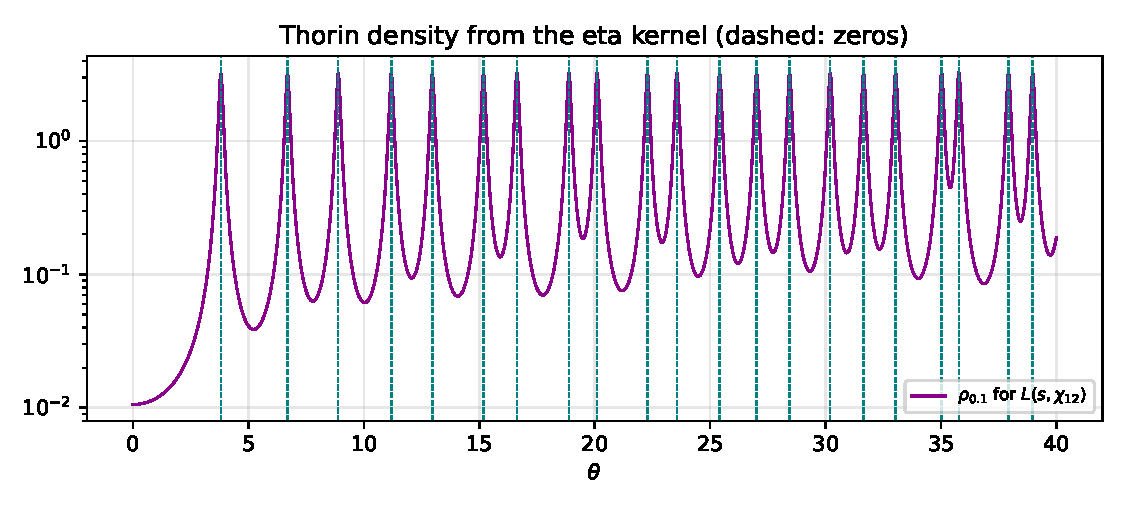
\includegraphics[width=0.95\textwidth]{fig/chi12.pdf}
\caption{The Thorin density $\rho_{0.1}$ of $L(s,\chi_{12})$ for $0\le\theta\le40$ on a logarithmic scale, computed from the Dedekind eta kernel, with the zeros dashed.}
\label{fig:ch16:rho}
\end{figure}

The zero density identity, Proposition~\ref{prop:zerodensity}, holds for $\xi(s,\chi_{12})$ with the same proof, since $\xi(s,\chi_{12})$ is entire, satisfies $\xi(s,\chi_{12})=\xi(1-s,\chi_{12})$, is positive on the real axis because $K$ is, and has no zeros with $\re s\ge1$. Its hypotheses are also the same: $T$ is not an ordinate, and no zero of $\xi(s,\chi_{12})$ lies on the segment from $\frac12+\varepsilon$ to $\frac12+\varepsilon+iT$, which is automatic at $\varepsilon=\frac12$. In it $N_{\chi_{12}}(T)$ counts the zeros with $0<\im\rho\le T$, and $\nu(\sigma,T)$ those among them with $\re\rho>\sigma$; $M_\varepsilon(T)=\int_0^T\rho_\varepsilon(\theta)\,d\theta$ is the Thorin mass up to height $T$, and $\tau_\varepsilon(T)$ is the change of argument of $\xi(s,\chi_{12})$ from $\frac12+\varepsilon+iT$ to $\frac12+iT$, divided by $\pi$. Table~\ref{tab:ch16:zd} evaluates the identity at $T=100$.

\begin{table}[htbp]
\centering\small
\begin{tabular}{rrrr}
\toprule
$\varepsilon$ & $M_\varepsilon(100)$ & $\tau_\varepsilon(100)$ & $M_\varepsilon+\tau_\varepsilon=N-2\nu$\\
\midrule
0.5 & 67.604974186 & $-0.604974186$ & 67.00000000000003\\
0.25 & 67.476432836 & $-0.476432836$ & 67.00000000010355\\
0.1 & 67.308171973 & $-0.308171973$ & 67.00000000014663\\
0.05 & 67.185437421 & $-0.185437421$ & 67.00000000009639\\
0.02 & 67.080023774 & $-0.080023774$ & 67.00000000005207\\
\bottomrule
\end{tabular}
\caption{The zero density identity for $L(s,\chi_{12})$ at height $100$, computed from the eta kernel. The last column is $N_{\chi_{12}}(100)-2\nu(\frac12+\varepsilon,100)$; the row $\varepsilon=\frac12$ gives $N_{\chi_{12}}(100)$.}
\label{tab:ch16:zd}
\end{table}

The row $\varepsilon=\frac12$ gives $N_{\chi_{12}}(100)=67$, and with the $67$ sign changes every zero below height $100$ is simple and lies on the critical line. The other rows give $\nu(\frac12+\varepsilon,100)=0$ without using the sign changes. This is GRH for $\chi_{12}$ below height $100$, read from the eta function alone. It is computed, not certified: the argument is followed on a grid as in Section~\ref{ch:turing}, in steps of $\varepsilon/8$ up the line of evaluation and in $2000$ steps along the horizontal segment, and its increments are summed in double precision. The deviations from $67$, at most $1.5\times10^{-10}$, are far below the one half that fixes the integer. GRH for small moduli has long been verified to far greater heights by other methods, by Rumely \cite{Rumely93} and later by Platt \cite{Platt16}.

\subsection{Ramanujan's \texorpdfstring{$\Delta$}{Delta} and the cost of the three evaluators}\label{sec:ch16:delta}

The same construction works for Ramanujan's cusp form $\Delta(z)=\eta(z)^{24}=\sum_{n\ge1}\tau(n)q^n$, $q=e^{2\pi iz}$, of weight $12$ and level $1$. Its $L$ function, normalised so that the critical line is $\re s=\frac12$, is $L(s,\Delta)=\sum_{n\ge1}\tau(n)n^{-s-11/2}$, and the completed function $\xi(s,\Delta)=(2\pi)^{-s-11/2}\Gamma(s+\frac{11}2)L(s,\Delta)$ satisfies $\xi(s,\Delta)=\xi(1-s,\Delta)$, since the root number of a level one form of weight $12$ is $i^{12}=1$. The Mellin transform of $\Delta(iy)$ gives the P\'olya type representation
\begin{gather*}
\xi\Big(\frac12+s,\Delta\Big)=\int_{\R}K_\Delta(u)\,e^{su}\,du,\\
K_\Delta(u)=e^{6u}\,\Delta(ie^u)=e^{6u}e^{-2\pi e^u}\prod_{n\ge1}\big(1-e^{-2\pi ne^u}\big)^{24}.
\end{gather*}
The kernel is even because $\Delta(i/y)=y^{12}\Delta(iy)$, positive by the product formula, and analytic in the strip $|\im u|<\pi/2$, twice as wide as that of the P\'olya kernel.

We computed $\tau(n)$ for $n\le3000$, the range needed for the prime weights of Section~\ref{sec:ch16:sin2}, as the coefficients of $\eta^{24}$ with integer polynomial arithmetic (checking $\tau(2)=-24$, $\tau(3)=252$, $\tau(11)=534612$), and evaluated the kernel by its $q$ expansion for $u\ge0$ and by evenness for $u<0$. At $60$ digits, with step $1/80$ and truncation $|u|\le4$, the trapezoid evaluator finds the first zeros on the critical line at
\[
9.222379,\ 13.907550,\ 17.442777,\ 19.656513,\ 22.336104,\ \dots,
\]
in agreement with the known values \cite[modular form 1.12.a.a]{LMFDB}, and $20$ sign changes below height $50$, the number of zeros there.

\label{sec:ch16:easier}Table~\ref{tab:ch16:cmp} compares this evaluator with those for $\zeta$ and $\chi_{12}$ at the same precision. In the variables of this section their steps are $1/40$ and $1/160$, and their truncations $|u|\le6$ and $|u|\le2.5$. The settings are not matched: the truncation is far longer than $60$ digits require for $\zeta$, and too short for them for $\chi_{12}$, whose kernel is still about $10^{-16}$ at $|u|=2.5$ (Section~\ref{sec:ch16:sin2}).

\begin{table}[htbp]
\centering\small
\setlength{\tabcolsep}{4pt}
\begin{tabular}{lccc}
\toprule
 & $\zeta$ & $L(s,\chi_{12})$ & $L(s,\Delta)$\\
\midrule
kernel & \begin{tabular}[t]{@{}c@{}}theta series with\\ terms of both signs\end{tabular} & \begin{tabular}[t]{@{}c@{}}$\eta$, a positive\\ product\end{tabular} & \begin{tabular}[t]{@{}c@{}}$\eta^{24}$, a positive\\ product\end{tabular}\\
decay of $\xi$ on the critical line & $e^{-\pi t/4}$ & $e^{-\pi t/4}$ & $e^{-\pi t/2}$\\
pole of $L$ & at $s=1$ & none & none\\
degree, conductor & $1$, $1$ & $1$, $12$ & $2$, $1$\\
zeros below height 50 & 10 & 28 & 20\\
first zero & 14.134725 & 3.804628 & 9.222379\\
digits lost per unit height & 0.31 & 0.36 & 0.59\\
digits lost per zero near height 40 & about 1 & about 0.5 & about 1\\
nodes & 481 & 801 & 641\\
time per point & 9.5 ms & 12.8 ms & 10.7 ms\\
\bottomrule
\end{tabular}
\caption{The trapezoid evaluators for $\zeta$, $L(s,\chi_{12})$ and $L(s,\Delta)$ at $60$ digits, with the settings given in the text. The decay of $\xi(\frac12+it)$ is shown up to a power of $t$; the digits lost per unit height are the slope of $\log_{10}|\xi(\frac12+it)|$ between heights $10.3$ and $40.3$; the times are per point, in \texttt{mpmath}.}
\label{tab:ch16:cmp}
\end{table}

The kernels are evaluated once, before the timing, so the times measure an exponential sum over the nodes and follow the node counts of the table rather than any intrinsic difference: the theta series, the eta series and the $q$ expansion of $\Delta$ all converge geometrically, with ratio at most $e^{-2\pi}$, once the modular symmetry is used. Per unit height $\Delta$ is the most expensive, because its gamma factor $\Gamma(s+\frac{11}2)$ decays like $e^{-\pi t/2}$ on the critical line, twice as fast as the $e^{-\pi t/4}$ of $\zeta$ and $\chi_{12}$: the untilted evaluator loses asymptotically $\pi/(2\log10)=0.68$ digits per unit height against $\pi/(4\log10)=0.34$. Between heights $10$ and $40$ the powers of $t$ in the completed functions and the size of $|L|$ at the two ends give the measured rates of the table. Tilting the contour to within $\delta$ of the edge of the strip reduces the loss to about $\delta\theta/\log10$ digits at height $\theta$ (Proposition~\ref{prop:tilt}, whose proof applies to both eta kernels), so the wider strip of the $\Delta$ kernel offsets its faster decay up to a factor polynomial in $1/\delta$; we have not run the tilted evaluator for $\Delta$. Per zero $L(s,\chi_{12})$ is the cheapest: its conductor packs the zeros at low height, $28$ below height $50$ against $10$ for $\zeta$, and it loses about half a digit per zero where $\zeta$ and $\Delta$ lose about one.

\subsection{The sine squared lemma without a pole}\label{sec:ch16:sin2}

The eta based functions differ from $\zeta$ in two structural ways. Their kernels are positive for an elementary reason, a product of factors $1-q^n$ with $0<q<1$, where the positivity of the P\'olya kernel $\Phi$ needs an argument (Section~\ref{ch:clock}). And their $L$ functions are entire, so two consequences of the pole of $\zeta$ disappear: the negative pole piece of the sine squared decomposition, and the factor that Chapters~\ref{chap:rzeta} and \ref{chap:rzid} need to remove the pole, which by Proposition~\ref{rz:prop:onlyhalf} alone prevents the normalised reciprocal zeta function from being a GGC. A floor in the sense of Theorem~\ref{rz:thm:floor} is still needed for $\chi_{12}$, since its tilt, the factor $e^{-c\sqrt u}$ in the variable $u$ of the clock (written $e^{-c\sqs}$ in Section~\ref{ch:rz2}), removes the negative part of the Thorin density of the gamma factor, and the gamma factor $(12/\pi)^{s/2}\Gamma(s/2)$ of $\xi(s,\chi_{12})$ is that of $\xi$ times $12^{s/2}$: Theorem~\ref{rz:thm:gammaggc} holds for it with $c=2.6861$ replaced by $c-\frac12\log12=1.4436$. The positivity of such a floor would need an analogue of Theorem~\ref{rz:thm:id}.

For $f=\chi_{12}$ or $\Delta$ write $\xi(s,f)=L_\infty(s,f)L(s,f)$, with $L_\infty$ the gamma factor, and $-(L'/L)(s,f)=\sum_{n\ge2}\Lambda_f(n)n^{-s}$ for $\re s>1$. At a basepoint $\alpha>1$ the sine squared lemma gives, as \eqref{eq:split} does for $\zeta$,
\begin{multline*}
v_\alpha(\theta)=\re\frac{\xi'}{\xi}(\alpha+i\theta,f)=\underbrace{\frac{\xi'}{\xi}(\alpha,f)}_{\text{drift}}+\underbrace{\re\frac{L_\infty'}{L_\infty}(\alpha+i\theta,f)-\frac{L_\infty'}{L_\infty}(\alpha,f)}_{\text{archimedean}\ \ge0}\\
+\underbrace{\sum_{n\ge2}\Lambda_f(n)\,n^{-\alpha}\,2\sin^2\Big(\frac{\theta\log n}2\Big)}_{\text{primes}},
\end{multline*}
where $v_\alpha(\theta)$ is $\pi$ times the Thorin density at resolution $\alpha-\frac12$, and the archimedean piece is nonnegative because the digamma function $\psi=\Gamma'/\Gamma$ satisfies $\re\psi(x+iy)\ge\psi(x)$ for $x>0$. For $\zeta$, whose gamma factor $\pi^{-s/2}\Gamma(1+\frac s2)$ absorbs the factor $s$ of $\xi$, the remaining factor $s-1$ adds the pole piece $\re\frac1{s-1}-\frac1{\alpha-1}$, which is $-\theta^2/\big((\alpha-1)((\alpha-1)^2+\theta^2)\big)$ at $s=\alpha+i\theta$, and the identity becomes \eqref{eq:split}.

The prime weights are $\Lambda(n)=\log p$ at $n=p^k$ for $\zeta$, all positive; $\Lambda_{\chi_{12}}(p^k)=\chi_{12}(p)^k\log p$ for $\chi_{12}$, of both signs and zero at $p=2$ and $3$; and $\Lambda_\Delta(p^k)=(\alpha_p^k+\bar\alpha_p^k)\log p$ for $\Delta$, where the Satake parameters $\alpha_p$ and $\bar\alpha_p$ are the roots of $X^2-\tau(p)p^{-11/2}X+1$. Deligne's theorem $|\tau(p)|\le2p^{11/2}$ \cite{Deligne74} makes them complex conjugates of modulus one, so the weights of $\Delta$ lie in $[-2\log p,2\log p]$ and take both signs.

We computed the three decompositions at $\alpha=2$ for $0\le\theta\le40$, with prime powers up to $3000$, and compared their sum with the left side computed from the kernel. They agree to $5\times10^{-4}$ for $\zeta$ and $9\times10^{-6}$ for $\Delta$, the difference being the truncation of the prime sum. For $\chi_{12}$ the largest difference, $2.5\times10^{-5}$ at $\theta=40$, is an error of the kernel evaluator, whose truncation at $|u|\le2.5$ is too short at that height. Of the $466$ prime power weights up to $3000$, none is negative for $\zeta$, $222$ are negative for $\chi_{12}$ (whose $18$ weights at powers of $2$ and $3$ vanish) and $230$ for $\Delta$.

\begin{figure}[htbp]
\centering
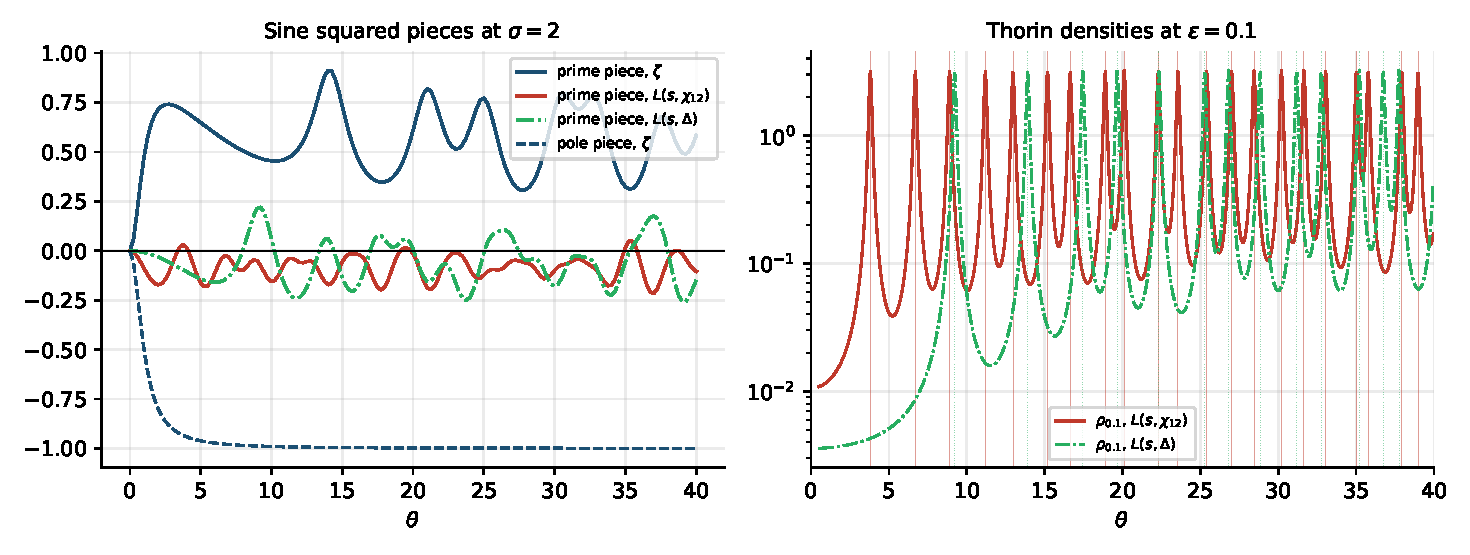
\includegraphics[width=\textwidth]{fig/lfunc.pdf}
\caption{Left: the prime pieces of the sine squared decomposition at the basepoint $\alpha=2$, written $\sigma$ in the plot, for $\zeta$, $L(s,\chi_{12})$ and $L(s,\Delta)$, and the pole piece of $\zeta$. For $\zeta$ the prime piece is positive and the pole piece negative; for the two eta based functions there is no pole piece and the prime piece takes both signs. Right: the Thorin densities $\rho_{0.1}$ of $L(s,\chi_{12})$ and $L(s,\Delta)$ on a logarithmic scale, peaking at their zeros (vertical lines).}
\label{fig:ch16:lfunc}
\end{figure}

On $0\le\theta\le40$ the prime piece of $\zeta$ ranges over $[0,0.915]$ and its pole piece over $[-0.999,0]$ (Figure~\ref{fig:ch16:lfunc}, left): the lemma writes the Thorin density as positive arithmetic mass minus one negative term. The prime piece of $L(s,\chi_{12})$ ranges over $[-0.218,0.053]$, and that of $L(s,\Delta)$ over $[-0.261,0.222]$. Their left sides are positive, with minima at $\theta=0$ equal to the drifts, $0.466$ and $0.167$, so the positivity comes from the drift and the archimedean piece, not from the primes.

For each of the three functions its Riemann hypothesis, RH for $\zeta$ and GRH for the other two, is the statement that $v_\alpha$ stays positive for every $\alpha>\frac12$; this is Lagarias's criterion \cite{Lagarias}, whose proof from the Hadamard product applies unchanged to $\xi(s,\chi_{12})$ and $\xi(s,\Delta)$. Below $\alpha=1$ the prime piece no longer converges absolutely. For $L(s,\chi_{12})$, Section~\ref{bp:eta:sec:below} shows that it still converges, as a limit over $n\le X$, when $L(s,\chi_{12})$ has no zeros to the right of some line $\re s=\alpha'$ with $\alpha'<\alpha$, and that conversely the convergence of the L\'evy form at the basepoint $\alpha$ forces the absence of zeros with $\re s>\alpha$; so the extension of the decomposition down to the centre is GRH for $\chi_{12}$. At resolution $0.1$ the Thorin densities of $L(s,\chi_{12})$ and $L(s,\Delta)$ have computed minima $0.011$ and $0.004$ below height $40$ (Figure~\ref{fig:ch16:lfunc}, right), positive as GRH predicts.

The distances of Section~\ref{ch:distances}, with the zeros of $L(s,\chi_{12})$ or $L(s,\Delta)$ as the reference atoms, Theorem~\ref{bs:thm:power} and the flow of Section~\ref{ch:dbn} carry over unchanged, the last two because they use only the Hadamard product, positivity on the real line and the decay of the kernel; we have not computed the first two for these functions, and Section~\ref{sec:ch16:dbn} computes the flow for $\Delta$. Theorem~\ref{bs:thm:power} also needs the bound $|\arg z|<\pi/4$ of Lemma~\ref{bs:lem:pair} for the zeros $z$ of $\xi(\frac12+iz,f)$ with $\re z>0$, and it holds here too: the zeros lie in the open critical strip, so $|\im z|<\frac12$, while the lowest ordinates, $3.80$ and $9.22$, exceed $\frac12$. The arithmetic side, however, offers no termwise positivity, even far to the right of the critical line, so the domination of the pole by positive primes that Sections~\ref{ch:motivation} and \ref{ch:sin2more} formulate for $\zeta$ has no direct analogue. Deligne's bound $|\Lambda_\Delta(n)|\le2\Lambda(n)$, like $|\Lambda_{\chi_{12}}(n)|\le\Lambda(n)$, bounds the prime piece below only by a multiple of minus the zeta prime piece, which tends to $-\infty$ as $\alpha\downarrow1$ for every $\theta\ne0$, and no domination argument follows from it. Far enough to the right the absolute values do suffice: the drift and the archimedean piece outweigh the prime piece bounded by the absolute values of its weights for $\alpha>1.8349$ for $L(s,\chi_{12})$ and for $\alpha>2.2823$ for the Dirichlet beta function $L(s,\chi_4)$, and by Kronecker's theorem no better bound from the sizes of the weights holds at all large heights (Propositions~\ref{prop:dbeta:termwise} and \ref{prop:dbeta:kron}). So although $L(s,\chi_{12})$ is the cheapest of the three functions per zero, neither eta based function is theoretically easier than $\zeta$: the sine squared lemma trades the negative pole term for a prime measure of both signs.

\subsection{Maxima of exponentials}\label{sec:ch16:max}

The product formula has a probabilistic reading, which the first author's note \cite{P26max} develops. The factor $1-e^{-2\pi ny}$ is the distribution function of an exponential variable with rate $2\pi n$, so
\[
F(y)=\prod_{n\ge1}\big(1-e^{-2\pi ny}\big)^{24}=e^{2\pi y}\Delta(iy),\qquad F_1(y)=\prod_{n\ge1}\big(1-e^{-2\pi ny}\big)=e^{\pi y/12}\eta(iy)
\]
are the distribution functions of the maxima $M^*$ and $M_1$ of independent exponential variables, $24$ of each rate $2\pi n$ for $M^*$ and one of each rate for $M_1$. Section~\ref{sec:maxexp:rep} turns the Mellin integral of $\Delta$ into an expectation over the law of $M^*$, a representation of $L(s,\Delta)$ with no signs, and compares it with the incomplete gamma continuations of Riemann and Hecke; Section~\ref{sec:maxexp:products} carries the construction to other products, and Section~\ref{sec:maxexp:gamma} reads it at real points as a statement about gamma mixtures. The last two parts study the laws themselves. That of $M_1$ is explicit: it is infinitely divisible, lies in the Bondesson class and is not a GGC (Section~\ref{sec:maxexp:M1}). That of $M^*$ is not even in the Bondesson class, because its Laplace transform has zeros off the real axis (Section~\ref{sec:maxexp:Mstar}).

\subsubsection{The max representation}\label{sec:maxexp:rep}

\begin{lemma}\label{lem:maxexp:max}
Let $E_{n,j}$, $n\ge1$, $1\le j\le24$, be independent, with $E_{n,j}$ exponential of rate $2\pi n$, and put $M^*=\sup_{n,j}E_{n,j}$ and $M^{(j)}=\sup_nE_{n,j}$. Almost surely these suprema are attained and finite, $\Pr(M^*\le y)=F(y)$ for $y>0$, and each $M^{(j)}$ has the distribution function $F_1$. So $M^*=\max_{j\le24}M^{(j)}$ is the maximum of $24$ independent copies of $M_1$.
\end{lemma}

\begin{proof}
For $y>0$, $\sum_{n,j}\Pr(E_{n,j}>y)=24\sum_ne^{-2\pi ny}<\infty$, so by the Borel Cantelli lemma only finitely many $E_{n,j}$ exceed $y$, almost surely. Taking $y$ rational and below $E_{1,1}$, the supremum is the largest of finitely many values. By independence $\Pr(M^*\le y)=\lim_N\prod_{n\le N}(1-e^{-2\pi ny})^{24}=F(y)$, and in the same way each $M^{(j)}$ has the distribution function $F_1$; the $M^{(j)}$ are independent because they are built from disjoint sets of the $E_{n,j}$.
\end{proof}

The modular relations $\Delta(i/y)=y^{12}\Delta(iy)$ and $\eta(i/y)=\sqrt y\,\eta(iy)$ become self dualities of the two laws,
\begin{equation}\label{eq:maxexp:dual}
F(y)=y^{-12}e^{2\pi y-2\pi/y}F(1/y),\qquad F_1(y)=y^{-1/2}e^{\pi y/12-\pi/(12y)}F_1(1/y),
\end{equation}
so the lower tails are thin: $\Pr(M^*\le y)\sim y^{-12}e^{-2\pi/y}$ and $\Pr(M_1\le y)\sim y^{-1/2}e^{-\pi/(12y)}$ as $y\downarrow0$. Since $F(1/y)\le1$, the first relation also gives $F(y)\le y^{-12}e^{2\pi y-2\pi/y}$ for every $y>0$, a bound that increases with $y$, because its logarithmic derivative is $(2\pi y^2-12y+2\pi)/y^2$ and $144<16\pi^2$.

The density of $M^*$ is Ramanujan's logarithmic derivative. Expanding $1/(1-e^{-2\pi ny})$ gives $(\log F)'(y)=24\sum_n2\pi n\,e^{-2\pi ny}/(1-e^{-2\pi ny})=48\pi\sum_{m\ge1}\sigma(m)e^{-2\pi my}$, with $\sigma(m)$ the sum of the divisors of $m$, so that, with Eisenstein's series $E_2(z)=1-24\sum_{m\ge1}\sigma(m)e^{2\pi imz}$,
\begin{equation}\label{eq:maxexp:density}
f^*(y)=F(y)\,(\log F)'(y)=2\pi F(y)\big(1-E_2(iy)\big).
\end{equation}
Taking the logarithmic derivative of \eqref{eq:maxexp:dual} gives the functional equation of the density,
\[
f^*(1/y)=y^{12}e^{2\pi/y-2\pi y}\Big(\big(2\pi y^2-12y+2\pi\big)F(y)-y^2f^*(y)\Big),
\]
which in terms of $E_2$ is its quasi modularity, $E_2(i/y)=-y^2E_2(iy)+6y/\pi$. At $y=2$ the quotient $F'/F$ of the product, the form \eqref{eq:maxexp:density} and the functional equation applied at $y=\frac12$ give the same value, $f^*(2)=0.000525840326953580416712$, and the density integrates to one to the $30$ digits printed (\texttt{maxexp\_checks.py}).

\begin{theorem}\label{thm:maxexp:max}
For every complex $s$,
\begin{equation}\label{eq:ch16:max}
\xi(s,\Delta)=(2\pi)^{-s-\frac{11}2}\,\E\,\Gamma\big(s+\tfrac{11}2,2\pi M^*\big),\qquad L(s,\Delta)=\E\,Q\big(s+\tfrac{11}2,2\pi M^*\big),
\end{equation}
with $\Gamma(a,x)=\int_x^\infty e^{-v}v^{a-1}dv$ and $Q(a,x)=\Gamma(a,x)/\Gamma(a)$, and both expectations converge absolutely. In particular $L(s,\Delta)=0$ at the points $s=-\frac{11}2-k$, $k=0,1,2,\dots$, where $Q(-k,x)=0$.
\end{theorem}

\begin{proof}
Put $a=s+\frac{11}2$, so that $\xi(s,\Delta)=\int_0^\infty\Delta(iy)y^{a-1}dy$. Inserting $\Delta(iy)=e^{-2\pi y}\Pr(M^*\le y)=e^{-2\pi y}\E\,\mathbf 1\{M^*\le y\}$ and integrating in $y$ first gives $\E\int_{M^*}^\infty e^{-2\pi y}y^{a-1}dy=(2\pi)^{-a}\E\,\Gamma(a,2\pi M^*)$. Fubini's theorem applies: with $\sigma=\re a$, Tonelli's theorem gives $\E\int_{M^*}^\infty e^{-2\pi y}y^{\sigma-1}dy=\int_0^\infty\Delta(iy)y^{\sigma-1}dy$, which is finite for every real $\sigma$, since $\Delta(iy)$ decays exponentially as $y\to\infty$ and like $y^{-12}e^{-2\pi/y}$ as $y\downarrow0$. The same computation gives $\E|\Gamma(a,2\pi M^*)|\le\E\,\Gamma(\sigma,2\pi M^*)<\infty$. Dividing by $(2\pi)^{-a}\Gamma(a)$, with $1/\Gamma$ entire, gives the second identity, in which $Q(a,x)$, for fixed $x>0$, is the entire function $\Gamma(a,x)/\Gamma(a)$ of $a$. At $a=-k$ it vanishes, since $\Gamma(-k,x)$ is finite and $1/\Gamma(-k)=0$.
\end{proof}

\begin{corollary}[Gamma mixture and mixed Poisson forms]\label{cor:maxexp:forms}
Let $G_a$ be a gamma variable of shape $a>0$ and scale one, and $N$ a Poisson process of unit rate, both independent of $M^*$. For real $s>-\frac{11}2$, with $a=s+\frac{11}2$,
\[
L(s,\Delta)=\Pr\big(G_a>2\pi M^*\big)=\E F\Big(\frac{G_a}{2\pi}\Big)=\E\prod_{n\ge1}\big(1-e^{-nG_a}\big)^{24},
\]
and for every integer $k\ge1$
\[
L\big(k-\tfrac{11}2,\Delta\big)=\Pr\big(N(2\pi M^*)\le k-1\big)=\E\Big[e^{-2\pi M^*}\sum_{j<k}\frac{(2\pi M^*)^j}{j!}\Big].
\]
\end{corollary}

\begin{proof}
For real $a>0$, $Q(a,x)=\Pr(G_a>x)$, which gives the first form; conditioning on $G_a$ instead gives $\Pr(M^*<G_a/2\pi)=\E F(G_a/2\pi)$, since the law of $M^*$ has no atoms. For an integer $k$ the $k$th point of $N$ has the law of $G_k$, so $\Pr(G_k>x)=\Pr(N(x)\le k-1)$. As a check, $F(y)=\sum_{n\ge1}\tau(n)e^{-2\pi(n-1)y}$ and $\E e^{-(n-1)G_a}=n^{-a}$ return the Dirichlet series $\sum_n\tau(n)n^{-a}$ term by term when $a>\frac{13}2$, where it converges absolutely.
\end{proof}

So $L(-\frac92,\Delta)=\E e^{-2\pi M^*}=0.03744128126851554174$ is a value of the Laplace transform of $M^*$, and the central value $L(\frac12,\Delta)=0.79212283864603056936$ is the probability that a Poisson clock of rate $2\pi$ rings at most five times before the time $M^*$. Write $P_k=\Pr(N(2\pi M^*)\le k-1)=L(k-\frac{11}2,\Delta)$. The functional equation $\xi(s,\Delta)=\xi(1-s,\Delta)$ at $s=k-\frac{11}2$ becomes the family of identities
\begin{equation}\label{eq:maxexp:fe}
(2\pi)^{-k}(k-1)!\,P_k=(2\pi)^{k-12}(11-k)!\,P_{12-k},\qquad1\le k\le11,
\end{equation}
both sides being $\xi(k-\frac{11}2,\Delta)$, which are nontrivial statements about the law of a maximum of exponential variables. Table~\ref{tab:maxexp:poisson} lists the probabilities, computed by quadrature against the density \eqref{eq:maxexp:density}; the two sides of \eqref{eq:maxexp:fe} agree to $10^{-43}$, and with Hecke's formula below to all $25$ digits printed. The gamma mixture form gives $L(0,\Delta)=\E F(G_{11/2}/2\pi)=0.7347229296103482203473$, and the max representation gives $L(\frac{17}2,\Delta)=0.998583063162746176491918$ and $L(\frac{29}2,\Delta)=0.999977182799369841174879$, in agreement with Hecke's formula and with the Dirichlet series.

\begin{table}[htbp]
\centering\small
\begin{tabular}{rcc}
\toprule
$k$ & $P_k=\Pr\big(N(2\pi M^*)\le k-1\big)=L(k-\frac{11}2,\Delta)$ & $(2\pi)^{-k}(k-1)!\,P_k=\xi(k-\frac{11}2,\Delta)$\\
\midrule
$1$ & $0.0374412812685$ & $0.00595896498958$\\
$2$ & $0.146374542091$ & $0.00370771046495$\\
$3$ & $0.315241565881$ & $0.00254175605420$\\
$4$ & $0.501617647511$ & $0.00193109920049$\\
$5$ & $0.666709188434$ & $0.00163398603484$\\
$6$ & $0.792122838646$ & $0.00154487936040$\\
$7$ & $0.877354125389$ & $0.00163398603484$\\
$8$ & $0.930707030298$ & $0.00193109920049$\\
$9$ & $0.962126459694$ & $0.00254175605420$\\
$10$ & $0.979809088251$ & $0.00370771046495$\\
$11$ & $0.989432913100$ & $0.00595896498958$\\
\bottomrule
\end{tabular}
\caption{The probabilities that a Poisson clock of rate $2\pi$ rings fewer than $k$ times before $M^*$, and the identities \eqref{eq:maxexp:fe}: the last column is symmetric about $k=6$. Computed by \texttt{maxexp\_checks.py}.}
\label{tab:maxexp:poisson}
\end{table}

\begin{remark}\label{rem:maxexp:fe}
The identities \eqref{eq:maxexp:fe} follow from the self duality \eqref{eq:maxexp:dual}, since $(2\pi)^{-k}(k-1)!\,P_k=\int_0^\infty e^{-2\pi y}F(y)y^{k-1}dy$ and the substitution $y\mapsto1/y$ turns this integral into the one with $12-k$ in place of $k$. They are five relations, since $k$ and $12-k$ give the same one and $k=6$ gives none, and they do not imply the self duality. Let $g$ be smooth and not identically zero, with compact support in $(0,1)$, such that $g(\log y)$ is orthogonal on $(1,e)$ to the five functions $e^{-2\pi y}F(y)(y^{k-1}-y^{11-k})$, $k\le5$. For small $\varepsilon$, $\tilde F(y)=F(y)\big(1+\varepsilon g(\log y)\big)$ is again a distribution function, because $F'$ has a positive lower bound and $F$ is below one on $[1,e]$, and it satisfies \eqref{eq:maxexp:fe}, because the perturbation changes the difference of the two sides of the $k$th identity by $\varepsilon$ times the integral of $g(\log y)$ against the $k$th function. It is not self dual: on $(1,e)$ self duality would give $\tilde F(y)=y^{-12}e^{2\pi y-2\pi/y}\tilde F(1/y)=F(y)$, since $g(\log(1/y))=0$. With $g$ even and supported in $(-1,1)$ instead, the same construction gives a self dual distribution function other than $F$, so self duality does not determine the law of $M^*$ either. What does determine it is self duality together with the form of $F$ as a power series in $e^{-2\pi y}$. If $F(y)=\sum_{n\ge0}c_ne^{-2\pi ny}$ for $y>0$, with $c_0=1$, and $F$ satisfies \eqref{eq:maxexp:dual}, then $f(z)=\sum_{n\ge0}c_ne^{2\pi i(n+1)z}$ is holomorphic on the upper half plane, satisfies $f(z+1)=f(z)$, and satisfies $f(-1/z)=z^{12}f(z)$ on the imaginary axis, hence everywhere by analytic continuation. So $f$ is a cusp form of weight $12$ for $\mathrm{SL}_2(\mathbb Z)$, a multiple of $\Delta$ because these cusp forms make up a space of dimension one \cite[Chapter 14]{IwaniecKowalski04}, and $c_0=1$ gives $f=\Delta$. This argument is the simplest case of Hecke's converse theorem \cite{Hecke36}, which recovers a modular form from the functional equation of its Dirichlet series. The distribution function of a maximum of independent exponential variables whose rates are integer multiples of $2\pi$ is a power series of this kind, so $M^*$ is the only such maximum with the self duality \eqref{eq:maxexp:dual}.
\end{remark}

Cutting the integral at $y=1$ and folding $(0,1)$ onto $(1,\infty)$ by modularity gives in the same way the symmetric form
\begin{gather}
\xi(s,\Delta)=A(s)+A(1-s),\qquad A(s)=\int_1^\infty\Delta(iy)\,y^{s+\frac92}dy,\label{eq:maxexp:sym}\\
A(s)=(2\pi)^{-s-\frac{11}2}\,\E\,\Gamma\big(s+\tfrac{11}2,2\pi\max(M^*,1)\big)=\sum_{n\ge1}\tau(n)\,\frac{\Gamma(s+\frac{11}2,2\pi n)}{(2\pi n)^{s+11/2}},\nonumber
\end{gather}
where the last form, Hecke's, comes from expanding $\Delta(iy)=\sum_n\tau(n)e^{-2\pi ny}$ instead. Hecke's form is the analogue for $\Delta$ of Riemann's second proof of the functional equation \cite[Chapter 1]{Edwards}, which cuts the Mellin integral of the theta function $\omega(x)=\sum_{n\ge1}e^{-\pi n^2x}$ of Section~\ref{ch:clock} at $x=1$ in the same way.

\begin{proposition}[Riemann]\label{prop:maxexp:riemann}
For every complex $s\ne0,1$,
\[
\pi^{-s/2}\Gamma\Big(\frac s2\Big)\zeta(s)=-\frac1s-\frac1{1-s}+\sum_{n\ge1}\Big[\frac{\Gamma(\frac s2,\pi n^2)}{(\pi n^2)^{s/2}}+\frac{\Gamma(\frac{1-s}2,\pi n^2)}{(\pi n^2)^{(1-s)/2}}\Big].
\]
\end{proposition}

\begin{proof}
For $\re s>1$, $\pi^{-s/2}\Gamma(\frac s2)\zeta(s)=\int_0^\infty\omega(x)x^{s/2-1}dx$. On $(0,1)$ substitute $x\mapsto1/x$ and use $\omega(1/x)=\sqrt x\,\omega(x)+\frac12\sqrt x-\frac12$, which is the theta transformation $1+2\omega(1/x)=\sqrt x\,(1+2\omega(x))$:
\[
\int_0^1\omega(x)x^{s/2-1}dx=\int_1^\infty\omega(x)x^{(1-s)/2-1}dx+\frac12\int_1^\infty x^{-(s+1)/2}dx-\frac12\int_1^\infty x^{-s/2-1}dx,
\]
and the last two integrals are $\frac1{s-1}$ and $-\frac1s$. On $(1,\infty)$ integrate $\omega$ term by term, with $\int_1^\infty e^{-\pi n^2x}x^{b-1}dx=(\pi n^2)^{-b}\Gamma(b,\pi n^2)$. The series converges uniformly on compact sets of $s$, because $\Gamma(b,\pi n^2)\le C_be^{-\pi n^2}(\pi n^2)^{\re b}$, so the identity continues to every $s\ne0,1$.
\end{proof}

At $s=2$ the right side gives $\pi/6$. At $s=\frac12+5i$ it gives a real number, as it must on the critical line, namely $-0.02182574236389736176$, and both values agree with the left side to $25$ digits. The three formulas are incomplete gamma continuations of Mellin integrals, but they randomise different things. In Riemann's and Hecke's the threshold is the fixed point $x=1$ or $y=1$, and the rates $\pi n^2$ or $2\pi n$ carry weights: one each for $\zeta$, at the price of the pole terms, and the signed coefficients $\tau(n)$ for $\Delta$. In \eqref{eq:ch16:max} there is a single rate $2\pi$, coming from the factor $q=e^{-2\pi y}$ of $\Delta$, and the threshold $M^*$ is random with a positive law; the symmetric form \eqref{eq:maxexp:sym} is Riemann's formula with the sum over $n$ replaced by an expectation over $\max(M^*,1)$, and with no pole terms. The max representation replaces Hecke's sum over the signed coefficients $\tau(n)$ by an expectation over a positive law.

The script \texttt{maxlaw.py} evaluates these expectations by quadrature against the density \eqref{eq:maxexp:density} of $M^*$ for $y\ge1$, with the self duality for $y<1$, so that $\tau$ enters only through the product. At $s=\frac12$, $\frac12+5i$ and $3$ the max representation, the symmetric form and Hecke's formula agree to the $25$ digits printed, for instance $\xi(\frac12,\Delta)=0.00154487936039502720604$. On the critical line $\xi(\frac12+i\theta,\Delta)=2\re A(\frac12+i\theta)$, and the symmetric form has its first zero at $\theta=9.2223793999211025222$. It also suggests a Hermite Biehler test, the route that Lagarias studied for $\xi$ \cite{Lagarias05}: if $|A(s)|>|A(1-s)|$ held throughout $\re s>\frac12$, there could be no zeros there. The test fails. At $\theta=0$ the half $A(s)$ dominates, with $|A(1-s)|/|A(s)|$ falling from $0.989$ at $\re s=0.52$ to $0.100$ at $\re s=4.5$, but on $\re s=0.6$ the two halves have equal modulus at $\theta=10.26$, $14.67$, $18.04$, $20.36$ and $22.99$, and the dominant half alternates between these ordinates, which separate the zeros $9.22$, $13.91$, $17.44$, $19.66$ and $22.34$. The curves of equal modulus are nearly vertical near the critical line and bend towards lower ordinates as $\re s$ grows (Figure~\ref{fig:maxexp:dominance}): on $\re s=4.5$ the first crossing is at $\theta=8.05$, and seven lie below height $25$ (\texttt{maxlaw.py}, \texttt{maxexp\_hb.py}). So the cut at $y=1$ gives no Hermite Biehler function.

The cut can be moved. For every $c>0$ the same folding gives $\xi(s,\Delta)=A_c(s)+A_{1/c}(1-s)$ with $A_c(s)=\int_c^\infty\Delta(iy)y^{s+9/2}dy$, and $c$ may be chosen separately on each horizontal ray. The script \texttt{maxexp\_hb.py} computes, for $0\le\theta\le25$ in steps of $0.05$, the best over $36$ cuts $c\in[0.35,1.2]$ of the least ratio $|A_c(s)|/|A_{1/c}(1-s)|$ over $120$ points of the ray $s=\sigma+i\theta$, $\frac12<\sigma\le14.5$. For $\theta\le12.9$ and $13.95\le\theta\le15.2$, and at $\theta=15.35$ and $15.4$, some cut dominates on the whole ray, for instance at $\theta=5$, $10.5$ and $12$ with least ratios $566$, $4.46$ and $2.03$, all for the smallest cut tried, $c=0.35$, where the cut at $1$ gives $1.0007$, $0.9065$ and $0.992$. For $12.95\le\theta\le13.9$, just below the zero $13.91$, at $\theta=15.25$ and $15.3$, and for $15.45\le\theta\le25$, no cut in the range dominates, the best least ratio staying between $0.9955$ and $1$. The freedom is in any case illusory. As $c\to0$, $A_{1/c}(1-s)\to0$ and $A_c(s)\to\xi(s,\Delta)$ uniformly on compact sets, so domination for small $c$ only says that $\xi(s,\Delta)$ does not vanish there, and the certificate turns into an evaluation of $\xi$; and at a zero $\frac12+i\gamma$ the two halves have equal modulus for every $c$, since their sum vanishes. A Hermite Biehler function that could prove GRH for $\Delta$ would have to come from the structure of the law of $M^*$, not from tuning a cut. The representation is exact and has no signs, but like the kernel it restates the problem without locating the zeros.

\begin{figure}[htbp]
\centering
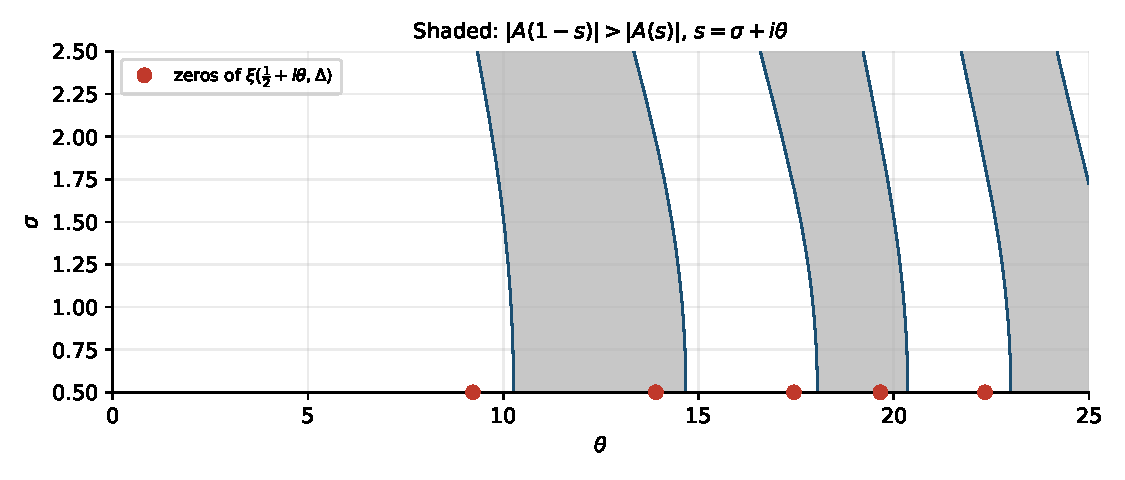
\includegraphics[width=0.8\textwidth]{fig/maxexp_dominance.pdf}
\caption{The Hermite Biehler test with the cut at $y=1$: shaded where $|A(1-s)|>|A(s)|$ for $s=\sigma+i\theta$, $\frac12<\sigma\le2.5$, with the curves of equal modulus and the zeros of $\xi(\frac12+i\theta,\Delta)$. Drawn by \texttt{maxexp\_figs.py}.}
\label{fig:maxexp:dominance}
\end{figure}

\subsubsection{Other theta products}\label{sec:maxexp:products}

The construction needs a modular form whose expansion on the imaginary axis is a power of $q$ times a product of factors $1-q^a$, $a>0$, with nonnegative exponents, so that the product is a distribution function; eta products with nonnegative exponents qualify.

For $\chi_{12}$ the Mellin integral of Section~\ref{sec:ch16:eta}, with $\eta(ix)=e^{-\pi x/12}F_1(x)$, gives in the same way
\[
L(s,\chi_{12})=\E\,Q\Big(\frac s2,\frac\pi{12}M_1\Big),\qquad\xi(s,\chi_{12})=A_{12}(s)+A_{12}(1-s),
\]
with $A_{12}(s)=\int_1^\infty\eta(ix)x^{s/2-1}dx=(\frac\pi{12})^{-s/2}\E\,\Gamma(\frac s2,\frac\pi{12}\max(M_1,1))$; the second exponent comes from $\eta(i/x)=\sqrt x\,\eta(ix)$. The factor $q^{1/24}$ of $\eta$ is what turns Euler's pentagonal exponents $k(3k\mp1)/2$ into the squares $n^2/24$, $n=6k\mp1$, and so produces the theta series, and the Dirichlet series, of a character. At $s=1$, where $Q(\frac12,x)=\operatorname{erfc}\sqrt x$, the class number formula reads $\E\operatorname{erfc}\sqrt{\pi M_1/12}=L(1,\chi_{12})=\log(2+\sqrt3)/\sqrt3$; at $s=2$, where $Q(1,x)=e^{-x}$, $L(2,\chi_{12})=\E e^{-\pi M_1/12}=\pi^2/(6\sqrt3)$ is a value of the Laplace transform of $M_1$, which Section~\ref{sec:maxexp:M1} computes in closed form; and at the centre $L(\frac12,\chi_{12})=\Pr(12G_{1/4}>\pi M_1)=0.498557002457815436157$. At $s=0.6+5i$ the max representation, both forms of the symmetric form and \texttt{mpmath}'s Dirichlet $L$ function agree to $25$ digits, with $\xi(0.6+5i,\chi_{12})$ as in Section~\ref{sec:ch16:eta}, and so do the three values above with their closed forms (\texttt{maxexp\_checks.py}, \texttt{maxlaw.py}).

For the elliptic curve of conductor $11$ the newform is $f(z)=\eta(z)^2\eta(11z)^2=q\prod_{n\ge1}(1-q^n)^2(1-q^{11n})^2=\sum_{n\ge1}a_nq^n$ \cite[modular form 11.2.a.a]{LMFDB}, so $f(iy)=e^{-2\pi y}F_{11}(y)$, where $F_{11}$ is the distribution function of the maximum $M_{11}$ of independent exponential variables, two of each rate $2\pi n$ and two of each rate $22\pi n$. The Fricke relation $f(i/(11y))=11y^2f(iy)$ makes $f(iy)$ decay faster than any power at both ends, and the proof of Theorem~\ref{thm:maxexp:max} gives, in the arithmetic normalisation $L(s,E)=\sum_na_nn^{-s}$ with centre $s=1$,
\[
L(s,E)=\E\,Q(s,2\pi M_{11})\quad\text{for every complex }s,\qquad L(1,E)=\E e^{-2\pi M_{11}}.
\]
So the central value is a value of the Laplace transform of $M_{11}$, and the max representation gives $L(1,E)=0.2538418608559106843378$, equal to all digits to the rapidly convergent series $2\sum_na_nn^{-1}e^{-2\pi n/\sqrt{11}}$ of root number one.

Jacobi's triple product gives $\vartheta_4(x)=\sum_{n\in\mathbb Z}(-1)^ne^{-\pi n^2x}=\prod_{m\ge1}(1-e^{-2\pi mx})(1-e^{-\pi(2m-1)x})^2$, a distribution function with no prefactor: that of the maximum $M_4$ of independent exponential variables, one of each rate $2\pi m$ and two of each rate $\pi(2m-1)$. The partial sums of the alternating series lie between $-1$ and $1$, so the series can be integrated term by term against $\theta e^{-\theta y}$, and the partial fraction expansion of $z/\sinh z$ gives
\[
\E e^{-\theta M_4}=\sum_{n\in\mathbb Z}(-1)^n\frac\theta{\theta+\pi n^2}=\frac{\sqrt{\pi\theta}}{\sinh\sqrt{\pi\theta}}=\prod_{n\ge1}\Big(1+\frac\theta{\pi n^2}\Big)^{-1},
\]
so $M_4\overset d=\sum_{n\ge1}E_n/(\pi n^2)$ with independent standard exponential variables $E_n$: a maximum of exponential variables that is also a sum of them, and a GGC with Thorin measure $\sum_n\delta_{\pi n^2}$. Since $\Pr(K\le k)=\sum_n(-1)^ne^{-2n^2k^2}=\vartheta_4(2k^2/\pi)$, $\pi M_4=2K^2$ has the Kolmogorov law of Table~\ref{tab:ch3:cat}. With no prefactor the Mellin transform gives moments instead of incomplete gamma functions: $\E M_4^{s/2}=\frac s2\int_0^\infty y^{s/2-1}(1-\vartheta_4(y))\,dy$ for $\re s>0$, and integrating $1-\vartheta_4(y)=2\sum_{n\ge1}(-1)^{n+1}e^{-\pi n^2y}$ term by term, for $\re s>1$ and then by analytic continuation, gives
\[
(1-2^{1-s})\,\zeta(s)=\frac{\E\big[(2K^2)^{s/2}\big]}{2\,\Gamma(1+\frac s2)}
\]
for every complex $s$, both sides being entire, since $\vartheta_4(y)=y^{-1/2}\sum_ne^{-\pi(n+\frac12)^2/y}$ makes every moment of $M_4$ finite. This is a case of the dictionary of Biane, Pitman and Yor \cite{BPY01}. At $s=1$ it gives $\E K=\sqrt{\pi/2}\,\log2=0.868731160636159141830$, which quadrature of $1-\vartheta_4$ reproduces to $2\times10^{-23}$; at $s=3$ and $\frac12+5i$ the two sides agree to $25$ digits, and $\E e^{-3M_4}=\sqrt{3\pi}/\sinh\sqrt{3\pi}=0.285645278943791835551$ by quadrature and in closed form.

For $\zeta$ itself the construction stops. The theta function $\vartheta_3(x)=1+2\omega(x)=\prod_{m\ge1}(1-q^{2m})(1+q^{2m-1})^2$, $q=e^{-\pi x}$, has factors larger than one and is not a distribution function, and the transformation $\vartheta_4(1/x)=\sqrt x\,\vartheta_2(x)$ leads to $\vartheta_2(x)=\sum_ne^{-\pi(n+\frac12)^2x}$, which is not one either. So the max structure reaches $\zeta$ only through the factor $1-2^{1-s}$, in moment form. It does not reach it through $\zeta_{\mathbb Q(\sqrt3)}(s)=\zeta(s)L(s,\chi_{12})$: the eta law represents the factor $L(s,\chi_{12})$ only, and no product of this kind can represent a Dedekind zeta function, since an eta product with nonnegative exponents decays faster than any power of $y$ at both ends of the imaginary axis, so its Mellin transform is entire, as in the proof of Theorem~\ref{thm:maxexp:max}, while $\zeta_{\mathbb Q(\sqrt3)}$ has a pole at $s=1$.

\subsubsection{Gamma shapes and infinite divisibility at real points}\label{sec:maxexp:gamma}

The P\'olya kernel of $\zeta$ and the kernel $K_\Delta$ of $\Delta$ differ in their gamma shapes. On the logarithmic scale the function $x^ae^{-x}$ of $x=ce^{ku}$ is proportional to the density of $(\log G_a-\log c)/k$, a log gamma density of shape $a$, and its Fourier transform $\int_{\R}x^ae^{-x}e^{i\theta u}du=k^{-1}c^{-i\theta/k}\Gamma(a+i\theta/k)$ has no zeros. With $x=2\pi e^u$, $K_\Delta(u)=e^{6u}\Delta(ie^u)=(2\pi)^{-6}x^6e^{-x}F(e^u)$ is a single gamma kernel of shape $6$ times the distribution function of $\log M^*$, and the gamma kernel's own transform is $(2\pi)^{-6-i\theta}\Gamma(6+i\theta)$, so every zero of $\xi(\frac12+i\theta,\Delta)$ is produced by the multiplier $F(e^u)$. The P\'olya kernel \eqref{eq:ch2:Phi} is, with $x_n=\pi n^2e^{2u}$ and the gamma densities $g_k(x)=x^{k-1}e^{-x}/\Gamma(k)$,
\[
\Phi(u)=2e^{u/2}\sum_{n\ge1}\big(2x_n^2-3x_n\big)e^{-x_n}=2e^{u/2}\sum_{n\ge1}\big(4g_3(x_n)-3g_2(x_n)\big),
\]
a signed mixture of Gamma(2) and Gamma(3) densities over the scales $\pi n^2$. As a function of $x=e^{2u}$ the sum is, up to the factor $x/2$, the density $2\sum_n(2\pi^2n^4x-3\pi n^2)e^{-\pi n^2x}$ of $\pi S_2/2$ in the representation $2\xi(s)=\E[(\pi S_2/2)^{s/2}]$ of Williams and of Biane, Pitman and Yor (Section~\ref{sec:ch19:williams}): a positive density that is a signed sum of gamma densities. On the logarithmic scale, with the weight $e^{u/2}=(x_n/\pi n^2)^{1/4}$, the two terms have shapes $\frac94$ and $\frac54$, while the theta function itself contributes $x_n^{1/4}e^{-x_n}$, of shape $\frac14$. The next remark shows where the two extra units come from.

\begin{remark}\label{rem:maxexp:shapes}
Let $D=-x\,d/dx$. Integrating by parts, $\int_0^\infty(Df)(x)x^{s/2-1}dx=\frac s2\int_0^\infty f(x)x^{s/2-1}dx$ whenever the boundary terms vanish, so the operator $2D(D-\frac12)$ corresponds to the factor $\frac12s(s-1)$ of $\xi(s)=\frac12s(s-1)\pi^{-s/2}\Gamma(\frac s2)\zeta(s)$. It annihilates $-\frac12$ and $\frac12x^{-1/2}$, the two terms by which $\omega(x)$ and $x^{-1/2}\omega(1/x)$ differ, and it maps $e^{-x}$ to $(2x^2-3x)e^{-x}$. Hence $[2D(D-\frac12)\omega](x)$, which is also $2D(D-\frac12)$ applied to $x^{-1/2}\omega(1/x)$, decays faster than any power at both ends,
\begin{gather*}
\xi(s)=\int_0^\infty\big[2D(D-\tfrac12)\omega\big](x)\,x^{s/2-1}dx\quad\text{for every }s,\\
\Phi(u)=2e^{u/2}\big[2D(D-\tfrac12)\omega\big](e^{2u}),
\end{gather*}
the first for $\re s>1$ by the integration by parts and then for every $s$ by analytic continuation, and the second by $x=e^{2u}$. So the gamma shapes of the terms $e^{-\pi n^2x}$ of $\omega$, one in $x$ and $\frac14$ on the logarithmic scale, are raised by one and by two, to the Gamma(2) and Gamma(3) of the P\'olya kernel, by the operator that removes the poles of $\zeta$. For $\Delta$, whose $L$ function is entire, no such operator is needed and the kernel keeps the single shape $6$; the cancellation between the Gamma(2) and Gamma(3) terms of $\Phi$ is replaced by the positive multiplier $F(e^u)$.
\end{remark}

At real points the Gamma(2) shape enters in a different way, through Kristiansen's theorem \cite{Kristiansen94}: every scale mixture of Gamma(2) laws, the law of $G_2V$ with $V\ge0$ independent of $G_2$, is infinitely divisible. Since $G_a\overset d=G_2B$ for $0<a<2$, with $B$ a beta variable of parameters $a$ and $2-a$ independent of $G_2$, the scale mixtures of Gamma($a$) laws with $a\le2$ are scale mixtures of Gamma(2) laws.

\begin{proposition}\label{prop:maxexp:krist}
For real $a>0$ let $W_a=G_a/(2\pi M^*)$, with $G_a$ independent of $M^*$. Then $W_a$ is a scale mixture of Gamma($a$) laws, the mixing law being that of $1/(2\pi M^*)$, and $L(a-\frac{11}2,\Delta)=\Pr(W_a>1)$. For $0<a\le2$, that is $-\frac{11}2<s\le-\frac72$, $W_a$ is infinitely divisible. In the same way $L(s,\chi_{12})=\Pr\big(12G_{s/2}/(\pi M_1)>1\big)$ for real $s>0$, where $12G_{s/2}/(\pi M_1)$ is infinitely divisible for $s\le4$, and is a mixture of exponential laws for $s\le2$, in particular at the centre $s=\frac12$.
\end{proposition}

\begin{proof}
The identities are Corollary~\ref{cor:maxexp:forms} and its analogue for $M_1$. For $a\le2$, $W_a=G_2\cdot B/(2\pi M^*)$ is a scale mixture of Gamma(2) laws, infinitely divisible by Kristiansen's theorem. For $s\le2$, $G_{s/2}\overset d=G_1B'$ with $B'$ a beta variable of parameters $\frac s2$ and $1-\frac s2$ (or $B'=1$ at $s=2$), so $12G_{s/2}/(\pi M_1)$ is a scale mixture of exponential laws, which is infinitely divisible by the theorem of Goldie and Steutel \cite{Goldie67,Steutel67}.
\end{proof}

At $a=2$ the proposition reads $L(-\frac72,\Delta)=\Pr(W_2>1)=\E\big[(1+2\pi M^*)e^{-2\pi M^*}\big]=0.146374542091266$, the Gamma(2) survival function averaged over $2\pi M^*$ (Table~\ref{tab:maxexp:poisson}). The proposition says nothing about zeros: the representation $\Pr(W_a>1)$ holds for real $a$ only, since on the critical line the shape $6+i\theta$ is not that of a probability law; for $\Delta$ the centre $a=6$ lies outside Kristiansen's range, while for $\chi_{12}$ the centre shape $\frac14$ lies inside it. The two Gamma(2) structures are also different in kind: the one in the P\'olya kernel is a kernel shape forced by the poles of $\zeta$, which governs the integrand on the critical line, and the one in Proposition~\ref{prop:maxexp:krist} is a mixing law, which governs a value at a real point.

\subsubsection{The law of \texorpdfstring{$M_1$}{M1}}\label{sec:maxexp:M1}

The law of $M_1$ is explicit. Put $b_n=\pi(n^2-1)/12$; the pentagonal number theorem of Section~\ref{sec:ch16:eta} reads $F_1(y)=\sum_{n\ge1}\chi_{12}(n)e^{-b_ny}$, so the rates in this expansion are $b_{6k\pm1}=\pi k(3k\pm1)$, $2\pi$ times the generalised pentagonal numbers $k(3k\pm1)/2$.

\begin{proposition}\label{prop:ch16:M1}
For $\theta>0$ let $w=\sqrt{1-12\theta/\pi}$, positive or purely imaginary. Then
\[
\E e^{-\theta M_1}=\frac{\pi(1-w^2)\sin(\pi w/3)}{2\sqrt3\,w\cos(\pi w/2)}=\prod_{k\ge1}\frac{1+\theta/b_{6k}}{(1+\theta/b_{6k-1})(1+\theta/b_{6k+1})}.
\]
\end{proposition}

\begin{proof}
Since $\sum_n\theta/(\theta+b_n)<\infty$, $\theta e^{-\theta y}F_1(y)$ can be integrated term by term, and $\theta+b_n=\pi(n^2-w^2)/12$ gives $\E e^{-\theta M_1}=\sum_{n\ge1}\chi_{12}(n)\theta/(\theta+b_n)=(1-w^2)\sum_{n\ge1}\chi_{12}(n)/(n^2-w^2)$. The function $g(w)=\pi\sin(\pi w/3)/(2\sqrt3\,w\cos(\pi w/2))$ is even and meromorphic, its only poles are simple and at the odd integers prime to $3$, and its residue at $w=n$ is $-\chi_{12}(n)/(2n)$, as for the series, so their difference is entire. On the circles $|w|=2k$, $|\cos(\pi w/2)|$ is bounded below, so $g=O(1/k)$ there, and the series is $O(k^{-1}\log k)$; by the maximum modulus principle the difference vanishes. For the product, insert $\sin(\pi w/3)=\frac{\pi w}3\prod_{m\ge1}(1-\frac{w^2}{9m^2})$ and $\cos(\pi w/2)=\prod_{n\text{ odd}}(1-\frac{w^2}{n^2})$. The factors with $n=3m$, $m$ odd, cancel, $1-w^2$ cancels the factor $n=1$, and what remains is a constant times the factors $1-w^2/n^2$ with $n=6k$ above and $n=6k\pm1$ below. The value $1$ at $\theta=0$ fixes the constant, and $(1-w^2/n^2)/(1-1/n^2)=1+\theta/b_n$.
\end{proof}

At $\theta=\pi/12$, where $w=0$, the closed form gives $\E e^{-\pi M_1/12}=\pi^2/(6\sqrt3)$, which is $L(2,\chi_{12})$ by Section~\ref{sec:maxexp:products}; the series in the proof reduces to $\sum_n\chi_{12}(n)n^{-2}$ there.

\begin{corollary}[A R\'enyi type identity]\label{cor:maxexp:renyi}
$M_1\overset d=\sum_{k\ge1}Y_k$ with independent $Y_k$, where $Y_k$ is exponential of rate $b_{6k-1}$ with probability $p_k$ and of rate $b_{6k+1}$ with probability $1-p_k$, and
\[
p_k=\Big(1-\frac{b_{6k-1}}{b_{6k}}\Big)\frac{b_{6k+1}}{b_{6k+1}-b_{6k-1}}=\frac{(12k-1)(3k+1)}{2(36k^2-1)},
\]
so $p_1=\frac{22}{35}$, $p_2=\frac{161}{286}$, and $p_k\downarrow\frac12$.
\end{corollary}

\begin{proof}
For $\alpha<\gamma<\beta$ the partial fractions $\frac{1+\theta/\gamma}{(1+\theta/\alpha)(1+\theta/\beta)}=p\frac\alpha{\alpha+\theta}+(1-p)\frac\beta{\beta+\theta}$ hold with $p=(1-\alpha/\gamma)\beta/(\beta-\alpha)$ and $1-p=\alpha(\beta-\gamma)/(\gamma(\beta-\alpha))$, both in $(0,1)$; take $\alpha=b_{6k-1}=\pi k(3k-1)$, $\gamma=b_{6k}=\pi(36k^2-1)/12$ and $\beta=b_{6k+1}=\pi k(3k+1)$ in each factor of Proposition~\ref{prop:ch16:M1}, and use the continuity theorem for Laplace transforms.
\end{proof}

By Frullani's integral, as in the first reading of Section~\ref{sec:ch3:readings}, the product gives
\[
-\log\E e^{-\theta M_1}=\int_0^\infty\big(1-e^{-\theta t}\big)\frac{k_1(t)}t\,dt,\quad k_1(t)=\sum_{k\ge1}\big(e^{-b_{6k-1}t}+e^{-b_{6k+1}t}-e^{-b_{6k}t}\big),
\]
so $M_1$ is infinitely divisible, with no drift and L\'evy density $k_1(t)/t$; this also follows from Corollary~\ref{cor:maxexp:renyi}, since mixtures of exponential laws are infinitely divisible \cite{Goldie67,Steutel67}. The L\'evy density is completely monotone, since $(e^{-b_{6k-1}t}-e^{-b_{6k}t})/t=\int_{b_{6k-1}}^{b_{6k}}e^{-zt}dz$, so $M_1$ lies in the Bondesson class BO of Section~\ref{sec:ch3:hierarchy}. It is not a GGC: its Thorin measure would have to be $U_1=\sum_k(\delta_{b_{6k-1}}+\delta_{b_{6k+1}}-\delta_{b_{6k}})$, negative at the points $b_{6k}$ where $\chi_{12}$ vanishes between $6k-1$ and $6k+1$. Concretely, the transform vanishes at $\theta=-b_{6k}$, where $w=6k$, so $-(\log\E e^{-\theta M_1})'$ has residue $-1$ there, and if $M_1$ were a GGC the Stieltjes inversion \eqref{eq:ch3:inversion} of this function would give $U(\{b_{6k}\})=-1$. The poles of the transform are at $\theta=-b_n$, $n\equiv\pm1\pmod6$, $n\ge5$, and its zeros at $-b_{6k}$: each zero lies between its own two poles $-b_{6k\pm1}$, but zeros and poles do not alternate, since $-b_7$ and $-b_{11}$, for instance, are consecutive poles. The next lemma, the Frullani identity behind Lemma~\ref{rz:lem:sin2} and the cosine dictionary \eqref{rz:eq:cosdict} read for a signed Thorin measure, turns this sign structure into a positivity statement.

\begin{lemma}\label{lem:maxexp:dict}
Let $X\ge0$ have Laplace exponent $-\log\E e^{-\theta X}=\int_{(0,\infty)}\log(1+\theta/z)\,U(dz)$ for a signed measure $U$ with $\int\log(1+1/z)\,|U|(dz)<\infty$, and put $N(z)=U((0,z])$, with $N(z)\log(1+u^2/z^2)\to0$ as $z\to\infty$ for real $u$. Then $-\log\E e^{-\theta X}=\int_0^\infty(1-e^{-\theta t})\nu(t)\,dt$ for $\theta\ge0$, with the signed function $\nu(t)=t^{-1}\int e^{-zt}U(dz)=\int_0^\infty e^{-zt}N(z)\,dz$, and for real $u$
\begin{equation}\label{eq:maxexp:three}
\begin{aligned}
-\log\big|\E e^{iuX}\big|^2&=\int_0^\infty4\sin^2\Big(\frac{ut}2\Big)\nu(t)\,dt\\
&=\int\log\Big(1+\frac{u^2}{z^2}\Big)U(dz)=\int_0^\infty N(z)\,\frac{2u^2}{z(z^2+u^2)}\,dz .
\end{aligned}
\end{equation}
The law of $X$ is a GGC if and only if $U\ge0$, and it lies in BO, that is, it is infinitely divisible with a completely monotone L\'evy density, if and only if $N\ge0$.
\end{lemma}

\begin{proof}
Frullani's integral $\log(1+\theta/z)=\int_0^\infty(1-e^{-\theta t})e^{-zt}t^{-1}dt$ gives the L\'evy form, the exchange of integrals being justified by $\log(1+\theta/z)\le C_\theta\log(1+1/z)$, and integrating $e^{-zt}$ against $dN$ by parts gives the second expression of $\nu$. The first equality of \eqref{eq:maxexp:three} is twice the real part of the L\'evy form at $\theta=-iu$, since $1-\cos ut=2\sin^2(ut/2)$; the second is the Frullani identity $\int_0^\infty4\sin^2(ut/2)e^{-zt}t^{-1}dt=\log(1+u^2/z^2)$; the third is an integration by parts, with $\frac d{dz}\log(1+u^2/z^2)=-2u^2/(z(z^2+u^2))$, whose boundary terms vanish by the assumptions. The signed function $\nu$ is determined by the law of $X$, since $t\nu(t)$ is the inverse Laplace transform of the derivative of $-\log\E e^{-\theta X}$, and so is the signed measure $U$, by the Stieltjes inversion of $\int U(dz)/(\theta+z)$. If $U\ge0$ the law is a GGC, and if it is a GGC, its Laplace exponent grows more slowly than $\theta$, so it has no drift, and its Thorin measure is $U$. If $N\ge0$, $\nu$ is completely monotone and the law is in BO; if the law is in BO, its L\'evy density is $\int e^{-zt}\mu(dz)$ with $\mu\ge0$, it equals $\nu$, and the uniqueness of Laplace transforms gives $\mu(dz)=N(z)\,dz$, so $N\ge0$, $N$ being right continuous.
\end{proof}

For $M_1$ the Thorin measure is $U_1=\sum_{n\ge2}a(n)\delta_{b_n}$ with weights of sine squared form,
\[
a(n)=\sin^2\frac{\pi n}2+\frac43\sin^2\frac{\pi n}3-1=\mathbf 1\{2\nmid n\}-\mathbf 1\{3\mid n\}=\frac16-\frac12\cos\pi n-\frac23\cos\frac{2\pi n}3,
\]
equal to $1$ for $n\equiv\pm1\pmod6$, to $-1$ for $6\mid n$, and to $0$ otherwise; each sine square is a combination of additive characters of $\mathbb Z/2$ or $\mathbb Z/3$, which makes Poisson summation available.

\begin{proposition}\label{prop:maxexp:levy}
The canonical function $k_1(t)=t\nu_1(t)$ of $M_1$ has the theta form
\[
k_1(t)=\tfrac12e^{\pi t/12}\Big(1+\frac{\vartheta_0-3\vartheta_{1/2}-4\vartheta_{1/3}}{\sqrt{3t}}\Big)-1,\qquad \vartheta_\alpha=\sum_{m\in\mathbb Z}e^{-12\pi(m+\alpha)^2/t},
\]
so $\nu_1(t)=(2\sqrt3)^{-1}t^{-3/2}-(2t)^{-1}+O(t^{-1/2})$ as $t\downarrow0$ and $\nu_1(t)\sim e^{-2\pi t}/t$ as $t\to\infty$. Its Bondesson function $N_1(z)=U_1((0,z])$ is nonnegative, and $N_1(z)\sim\frac13\sqrt{3z/\pi}$ as $z\to\infty$.
\end{proposition}

\begin{proof}
Since $a$ is even, $a(0)=-1$ and $a(1)=1$,
\[
k_1(t)=\sum_{n\ge2}a(n)e^{-b_nt}=\tfrac12e^{\pi t/12}\Big(1+\sum_{n\in\mathbb Z}a(n)e^{-\pi n^2t/12}\Big)-1.
\]
Poisson summation, $\sum_{n\in\mathbb Z}\cos(2\pi n\alpha)e^{-\pi n^2v}=v^{-1/2}\sum_{m\in\mathbb Z}e^{-\pi(m+\alpha)^2/v}$ with $v=t/12$, applied to the three terms of the cosine form of $a(n)$, gives the theta form. As $t\downarrow0$, $\vartheta_0=1+O(e^{-12\pi/t})$, while $\vartheta_{1/2}$ and $\vartheta_{1/3}$ are $O(e^{-4\pi/(3t)})$, so $k_1(t)=(2\sqrt{3t})^{-1}-\frac12+O(\sqrt t)$; as $t\to\infty$ the first term $e^{-b_5t}=e^{-2\pi t}$ of the series dominates. Since $b_{6k-1}<b_{6k}<b_{6k+1}$, every negative atom of $U_1$ is preceded by its own positive atom, so $N_1\ge0$. Up to $z$ there are about $X/3$ integers $n\equiv\pm1\pmod6$ and $X/6$ multiples of $6$ with $b_n\le z$, where $X=\sqrt{12z/\pi+1}$, so $N_1(z)=X/6+O(1)\sim\frac13\sqrt{3z/\pi}$; this agrees with the expansion at $0$, since $\nu_1(t)=\int_0^\infty e^{-zt}N_1(z)\,dz$ and $c\sqrt z$ gives $c\,\Gamma(\frac32)t^{-3/2}$.
\end{proof}

The L\'evy density has the index $\frac12$ of a Brownian first passage time, matching $-\log\E e^{-\theta M_1}\sim\sqrt{\pi\theta/3}$, which the lower tail $F_1(y)\sim y^{-1/2}e^{-\pi/(12y)}$ gives; this index comes from modularity. By \eqref{eq:maxexp:three}, the modulus of the characteristic function is
\[
\big|\E e^{iuM_1}\big|^{-2}=\prod_{k\ge1}\frac{(1+u^2/b_{6k-1}^2)(1+u^2/b_{6k+1}^2)}{1+u^2/b_{6k}^2}=\exp\int_0^\infty N_1(z)\,\frac{2u^2\,dz}{z(z^2+u^2)},
\]
the exponential of a positive kernel integrated against a nonnegative function. Figure~\ref{fig:maxexp:laws} (left) shows $N_1$ against its asymptote.

The sine squared form of $a(n)$ splits $U_1$ into two positive measures: $\sin^2(\pi n/2)$ selects the odd $n$, and $1-\frac43\sin^2(\pi n/3)$ the multiples of $3$. Each is the Thorin measure of a GGC.

\begin{theorem}\label{thm:maxexp:ggc}
With independent standard exponential variables $E_n$ and $E'_m$, let $S=\sum_{n\text{ odd},\,n\ge3}E_n/b_n$ and $Z=\sum_{m\ge1}E'_m/b_{3m}$, with $Z$ independent of $M_1$. Then $S$ and $Z$ are GGCs,
\[
\E e^{-\theta S}=\frac\pi4\,\frac{1-w^2}{\cos(\pi w/2)},\qquad \E e^{-\theta Z}=\frac{\sqrt3\,w/2}{\sin(\pi w/3)},
\]
and $M_1+Z\overset d=S$. Equivalently $U_1=U_S-U_Z$, with $U_S=\sum_{n\text{ odd},\,n\ge3}\delta_{b_n}$ and $U_Z=\sum_{m\ge1}\delta_{b_{3m}}$, the atoms at $b_{3m}$ with $m$ odd cancelling.
\end{theorem}

\begin{proof}
With $1+\theta/b_n=(n^2-w^2)/(n^2-1)$, the product $\cos(\pi w/2)=\prod_{n\text{ odd}}(1-w^2/n^2)$ gives $\prod_{n\text{ odd},\,n\ge3}(1+\theta/b_n)=\frac4\pi\cos(\pi w/2)/(1-w^2)$, the constant $\frac\pi4=\prod_{n\text{ odd},\,n\ge3}(1-n^{-2})$ being the limit at $w=1$; and $\sin(\pi w/3)/(\pi w/3)=\prod_m(1-w^2/9m^2)$ gives $\prod_m(1+\theta/b_{3m})=\frac2{\sqrt3}\sin(\pi w/3)/w$. The quotient of the two transforms is the closed form of Proposition~\ref{prop:ch16:M1}, so $\E e^{-\theta(M_1+Z)}=\E e^{-\theta S}$.
\end{proof}

The rates are shifted eigenvalues of Brownian hitting times \cite{BPY01}. With $\lambda_j=\pi^2(2j-1)^2/8$, the rates of the exit time $C$ of Brownian motion from $(-1,1)$, whose transform is $1/\cosh\sqrt{2\theta}=\prod_j(1+\theta/\lambda_j)^{-1}$, $b_{2j-1}=\frac2{3\pi}(\lambda_j-\lambda_1)$, so $S\overset d=\frac{3\pi}2\sum_{j\ge2}E_j/(\lambda_j-\lambda_1)$: the variable $C=\sum_jE_j/\lambda_j$ with its ground mode $j=1$ removed and the others shifted by $\lambda_1$. The law of $C$ tilted by $e^{cC}$, $c<\lambda_1$, is that of $\sum_jE_j/(\lambda_j-c)$, so $\frac2{3\pi}S$ is its limit at the critical tilt $c\uparrow\lambda_1$ with the diverging ground mode removed; the tilt itself has no limit, since $\E e^{\lambda_1C}=\infty$. With $\mu_m=\pi^2m^2/2$, the rates of the first passage $T$ of the three dimensional Bessel process from $0$ to $1$, whose transform is $\sqrt{2\theta}/\sinh\sqrt{2\theta}$, $b_{3m}=\frac3{2\pi}(\mu_m-\frac{\pi^2}{18})$, so $Z\overset d=\frac{2\pi}3T^{(\pi^2/18)}$, where $T^{(c)}$ has the law of $T$ tilted by $e^{cT}$, a proper law since $\frac{\pi^2}{18}<\mu_1$. The Kolmogorov law is the case with nothing to divide by: comparing transforms, $M_4=\frac\pi2T$ exactly. By Kent's theorem with Krein's inverse spectral theory (Section~\ref{sec:ch18:kent}), $S$ and $Z$, GGCs without drift whose Thorin measures are unit atoms at distinct points, are hitting times of levels by generalised diffusions started at a reflecting or entrance end, so
\[
M_1+\big(\text{a tilted Bessel first passage time}\big)\overset d=\big(\text{the reduced Brownian exit time }S\big),
\]
and the transform of $M_1$ is the quotient of the transforms of two hitting times; the character $\chi_{12}$ enters only through the quotient. $M_1$ itself is not a hitting time from such an end, since those are GGCs. Every first hitting time of a one dimensional diffusion lies in BO \cite{Kent82}, as $M_1$ does, and from an interior point the transform is a quotient of the kind discussed in Section~\ref{sb:sec:bernstein}; whether $M_1$ is the hitting time of some level by some diffusion started at an interior point we do not know.

At $\theta=2$ and $1+3i$, \texttt{maxlaw.py} finds the closed form of Proposition~\ref{prop:ch16:M1}, the product and the quadrature of $F_1$ in agreement to $25$ digits, for instance $\E e^{-2M_1}=0.6942503501538752318025$, and the same for $S$ and $Z$, with $\E e^{-\theta M_1}\E e^{-\theta Z}/\E e^{-\theta S}-1$ below $3\times10^{-41}$. At $u=5$, $-\log|\E e^{iuM_1}|^2=0.40295014525377167405$ from the closed form, from the law of $M_1$ and from the Thorin sum $\int\log(1+u^2/z^2)U_1(dz)$, and to $18$ digits from the integral of $N_1$ in \eqref{eq:maxexp:three}; $N_1$ is nonnegative over the first $60000$ atoms, where it reaches $20000$ against the asymptote $20000.17$; and the theta form of $k_1$ agrees with the series to $20$ digits at $t=0.01$, $0.05$, $0.1$, $0.3$, $1$, $2$ and $3$. At $\theta=2$ the derivative $-(\log\E e^{-\theta M_1})'=\int U_1(dz)/(\theta+z)$ is $0.16796840787856222484$ in closed form and as the sum over the Thorin atoms, and $\int N_1(z)(2+z)^{-2}dz$ agrees to $2\times10^{-15}$, the error of truncating the integral; the Laplace exponent at $\theta=2$ is $0.36492264843255339528$ in closed form and as the L\'evy integral $\int_0^\infty(1-e^{-2t})\nu_1(t)\,dt$. The expansion of $\nu_1$ checks too: $2t(\nu_1(t)-(2\sqrt3)^{-1}t^{-3/2})$ is $-0.9985$, $-0.99985$ at $t=10^{-4}$, $10^{-6}$, and $t\nu_1(t)e^{2\pi t}$ is $0.99685$, $0.9999994$ at $t=2$, $5$ (\texttt{maxlaw.py}, \texttt{maxexp\_checks.py}).

\subsubsection{The law of \texorpdfstring{$M^*$}{M*}}\label{sec:maxexp:Mstar}

The law of $M^*$ has no such product, but its transform $\psi^*(\theta)=\E e^{-\theta M^*}=\theta\int_0^\infty e^{-\theta y}F(y)\,dy$ is meromorphic: since $F(y)=\sum_{n\ge1}\tau(n)e^{-2\pi(n-1)y}$, for any $c>0$
\[
\psi^*(\theta)=\theta\int_0^ce^{-\theta y}F(y)\,dy+\theta\sum_{n\ge1}\tau(n)\frac{e^{-(\theta+2\pi(n-1))c}}{\theta+2\pi(n-1)},
\]
with at most simple poles at $\theta=-2\pi m$, $m\ge1$, of residue $-2\pi m\,\tau(m+1)$. Just to the right of a pole $\psi^*$ has the sign of the residue and just to the left the opposite sign, so it has a real zero between $-2\pi(m+1)$ and $-2\pi m$ whenever $\tau(m+1)\tau(m+2)>0$. The first such pair is $\tau(6)=-6048$, $\tau(7)=-16744$, and \texttt{maxlaw.py}, with $c=0.3$ at $40$ digits, finds the zero at $\theta=-34.4840085134049704852=-2\pi\times5.48830041253$. It is the only sign change of $\psi^*$ on $(-15\pi,0)$, and the argument principle on the rectangle $|\re\theta|\le15\pi$, $|\im\theta|\le60$, which contains the seven poles $-2\pi,\dots,-14\pi$, gives winding number $-6$, so it is the only zero there. As for $M_1$, the zero shows that $M^*$ is not a GGC.

Farther out the zeros leave the real axis. The script \texttt{maxexp\_psizeros.py} evaluates $\psi^*$ from the cut form with $c=0.08$, the integral by Gauss Legendre quadrature and the series to $n=900$, at $230$ bits, and checks it against $c=0.05$ to a relative $10^{-55}$. It then certifies the zeros in ball arithmetic, with $c=\frac3{100}$, the series to $n=1500$, its tail bounded by Deligne's bound $|\tau(n)|\le d(n)n^{11/2}\le2n^6$, and the integral bounded by $F(y)\le y^{-12}e^{2\pi y-2\pi/y}$, which is increasing.

\begin{proposition}\label{prop:maxexp:psizeros}
\begin{enumerate}
\item For each of the $25$ values $m\le60$ with $\tau(m+1)\tau(m+2)>0$, $\psi^*$ changes sign in an interval of length $2\times10^{-20}$ inside the gap $(-2\pi(m+1),-2\pi m)$; the zeros begin $\theta/2\pi=-5.48830041$, $-8.66373325$, $-11.4203774$, $-13.2533839$, $-14.7973058$, and the last is $-60.7670708$.
\item $\psi^*$ has exactly one zero in the disc of radius $10^{-7}$ about each of the ten points
\[
\begin{aligned}
&-155.5940822775511402804\pm2.7631188861212609656\,i,\\
&-215.6211277570694988944\pm2.9647292148515237348\,i,\\
&-307.4008549057072052743\pm3.2283287024583906394\,i,\\
&-322.6135369899940182007\pm3.0449254921259967464\,i,\\
&-347.8816009468099010890\pm2.7171007701068929577\,i,
\end{aligned}
\]
and it lies within $10^{-19}$ of that point.
\end{enumerate}
\end{proposition}

\begin{proof}
For (1), the values of $\psi^*$ at the two ends of each interval are balls of opposite signs. For (2), let $z_0$ be the approximation to the zero computed by Newton's method at $230$ bits; the point shown is $z_0$ rounded to nineteen decimals, at distance at most $6.1\times10^{-20}$ from it. With $A\ge|\psi^*(z_0)|$, $B\le|{\psi^*}'(z_0)|$ and $C\ge|{\psi^*}''|$ on the square of half side $r$ about $z_0$, each computed as a ball, $A+2Cr^2<Br/2$ holds for $r=10^{-6}$ and for $r=10^{-29}$. On the circle $|\theta-z_0|=r$, inside the square, $|\psi^*(\theta)-{\psi^*}'(z_0)(\theta-z_0)|\le A+Cr^2/2<Br$, so by Rouch\'e's theorem $\psi^*$ has as many zeros in the disc $|\theta-z_0|<r$ as ${\psi^*}'(z_0)(\theta-z_0)$, namely one. The disc of radius $10^{-7}$ about the point shown lies in the disc of radius $10^{-6}$ about $z_0$, and the disc of radius $10^{-29}$ about $z_0$ lies within $10^{-19}$ of the point shown. The zeros come in conjugate pairs because $\psi^*$ is real on the real axis.
\end{proof}

The argument principle on the rectangles $|\re\theta|\le2\pi(k+\frac12)$, with $|\im\theta|\le30$ for $k=15$, $25$, $40$ and $60$ and $|\im\theta|\le100$ for $k=60$, and on a grid of cells, $2\pi$ wide and at most $5$ high, covering $-2\pi\times60.5\le\re\theta\le2\pi\times5.5$, $\frac12\le\im\theta\le30$, finds exactly these zeros: the winding number on the largest rectangle, which contains the $60$ poles $-2\pi,\dots,-120\pi$, is $-26$, so it contains $34$ zeros, the $24$ real zeros with $m\le59$ and the ten nonreal zeros of the proposition. This count, unlike the zeros themselves, is computed and not certified: the change of argument is followed along the contours with steps halved until it is below $0.3$, in ball arithmetic whose radii stay below a relative $10^{-46}$. Every real zero lies in a gap where the residues force it, every gap with $\tau(m+1)\tau(m+2)<0$ is free of real zeros, and the five nonreal pairs have their real parts in such gaps, those with $m=24$, $34$, $48$, $51$ and $55$ ($\re\theta/2\pi=-24.764$, $-34.317$, $-48.924$, $-51.346$, $-55.367$), at heights between $2.72$ and $3.23$ (Figure~\ref{fig:maxexp:laws}, right). In a gap where the residues have opposite signs, $\psi^*$ has the same sign at both ends, so its real zeros there come in pairs; the computation finds none, and the five nonreal pairs sit in such gaps, as if a pair of real zeros had collided and left the axis.

\begin{corollary}\label{cor:maxexp:notBO}
$M^*$ is not in the Bondesson class BO; in particular it is not a GGC.
\end{corollary}

\begin{proof}
If $M^*$ were in BO, its L\'evy density would be $\int e^{-zt}\mu(dz)$ with $\mu\ge0$, so $-(\log\psi^*)'(\theta)=d+\int\mu(dz)(\theta+z)^{-2}$, with $d\ge0$ the drift, for $\theta>0$. The right side is holomorphic on $\cut$, since $\int\mu(dz)(1+z)^{-2}<\infty$ and $|\theta+z|$ is bounded below by a multiple of $1+z$ for $\theta$ in a compact subset of $\cut$. Then the meromorphic function ${\psi^*}'/\psi^*$ would have no poles in $\cut$, and $\psi^*$ no zeros there, against Proposition~\ref{prop:maxexp:psizeros}(2).
\end{proof}

Nor does $M^*$ have a signed Thorin measure in the sense of Lemma~\ref{lem:maxexp:dict}: for a signed measure $U$ on $(0,\infty)$, $-(\log\psi^*)'(\theta)=\int U(dz)(\theta+z)^{-1}$ would again be holomorphic on $\cut$. Unit atoms at the points $2\pi m$ with $\tau(m+1)\ne0$, less unit atoms at the real zeros, account for the poles and the real zeros of $\psi^*$, but no measure on the positive axis accounts for the nonreal zeros. Whether $M^*$ is infinitely divisible remains open. If it is, with L\'evy measure $\nu^*$, then $-(\log\psi^*)'(\theta)=d+\int t\,e^{-\theta t}\nu^*(dt)$ is completely monotone on $(0,\infty)$: the cumulants $\kappa_j(\theta)=(-1)^j(\log\psi^*)^{(j)}(\theta)$ of $M^*$ tilted by $e^{-\theta M^*}$ are all positive. At $\theta=0.5$, $2$, $8$ and $30$ the first eight are positive, for instance $0.54374$, $0.025649$, $0.0045870$, $0.0014574$ for $j\le4$ at $\theta=2$, as the first author's note found. As $\theta\to\infty$ the Laplace method, at the saddle point $y_0=\sqrt{2\pi/\theta}$ of $e^{-\theta y-2\pi/y}$ and with the lower tail $F(y)\sim y^{-12}e^{-2\pi/y}$, gives
\[
\psi^*(\theta)\sim2^{-1/2}(2\pi)^{-21/4}\,\theta^{25/4}\,e^{-2\sqrt{2\pi\theta}},
\]
so $-\log\psi^*(\theta)=2\sqrt{2\pi\theta}-\frac{25}4\log\theta+\frac{21}4\log2\pi+\frac12\log2+o(1)$; the ratio of $\psi^*$ to the right side is $2.33$, $1.32$ and $1.094$ at $\theta=10^3$, $10^4$ and $10^5$, consistent with a correction of order $\theta^{-1/2}$. If $M^*$ is infinitely divisible, it has no drift, and Karamata's Tauberian theorem turns the leading term into $\nu^*((t,\infty))\sim2\sqrt2\,t^{-1/2}$ as $t\downarrow0$, the behaviour of the L\'evy measure $\sqrt2\,t^{-3/2}dt$ of the first passage time of Brownian motion to the level $2\sqrt\pi$.

The first author conjectures that every maximum of independent exponential variables is infinitely divisible \cite{P26max}; $M_1$, $M_4$, $M^*$ and $M_{11}$ are of this kind. For finitely many rates $\lambda_1,\dots,\lambda_n$ the transform is rational: with $\lambda_S=\sum_{i\in S}\lambda_i$,
\[
\E e^{-\theta M}=\theta\int_0^\infty e^{-\theta y}\prod_{i\le n}(1-e^{-\lambda_iy})\,dy=\sum_{S\ne\emptyset}(-1)^{|S|+1}\frac{\lambda_S}{\theta+\lambda_S},
\]
with simple poles at the values $-\lambda_S$ whose grouped coefficients do not vanish, generically $2^n-1$ of them, and, since $\E e^{-\theta M}\sim n!\,\lambda_1\cdots\lambda_n\theta^{-n}$, with $n$ fewer zeros. Writing the poles as $-p$ and the zeros as $-z$, Frullani's integral gives $-\log\E e^{-\theta M}=\int_0^\infty(1-e^{-\theta t})k(t)t^{-1}dt$ with $k(t)=\sum_pe^{-pt}-\sum_ze^{-zt}$, as long as every zero has $\re z>0$, and by the uniqueness of the L\'evy measure the law is infinitely divisible if and only if $k\ge0$. In particular infinite divisibility forces every zero to have $\re z$ at least the smallest pole $p_{\min}$, since otherwise $k$ would change sign at large $t$. For two rates $a<b$ the transform is $ab(a+b+2\theta)/((a+\theta)(b+\theta)(a+b+\theta))$ and the canonical function is $e^{-at}+e^{-bt}+e^{-(a+b)t}-e^{-(a+b)t/2}$, positive by the inequality of arithmetic and geometric means; the signed Thorin measure $\delta_a+\delta_b+\delta_{a+b}-\delta_{(a+b)/2}$ has a nonnegative distribution function, so this maximum is in BO and is not a GGC, and $e^{at}k(t)=1-x+x^2+x^{2b/(b-a)}>\frac34$ with $x=e^{-(b-a)t/2}$, a bound approached as $b/a\downarrow1$ (at $b=a$ the zero cancels the pole at $-a$, and $e^{at}k(t)=1+e^{-at}$). The script \texttt{maxexp\_checks.py} groups the exponents exactly, finds the zeros at $40$ digits and evaluates $k$ at $181$ points of $p_{\min}t\in[10^{-3},40]$, for $300$ families of random rational rates in $[0.1,5]$ for each $n=2,3,4,5$ and $40$ families with $n=6$. In every family $k$ is positive at every point, $e^{p_{\min}t}k(t)\ge0.53$, and every zero has $\re z>p_{\min}$. Nonreal zeros are common: they occur in $140$, $222$, $266$ and $40$ of the families with $3$, $4$, $5$ and $6$ rates, up to $2$, $8$, $22$ and $52$ of them. So nonreal zeros, which exclude BO, do not seem to exclude infinite divisibility. The truncations of $M_1$, with the rates $2\pi n$, $n\le N$, have only real zeros for $N=4,\dots,10$, and those of $M^*$, with each rate $2\pi n$, $n\le N$, taken $24$ times, have $24$ real zeros for $N=2$ and $72$ zeros, $52$ of them nonreal, for $N=3$; in each case $k$ is positive on the grid. None of this is a proof.

\begin{question}\label{q:maxexp:id}
Is every maximum of independent exponential variables infinitely divisible? In particular, is $M^*$?
\end{question}

\begin{figure}[htbp]
\centering
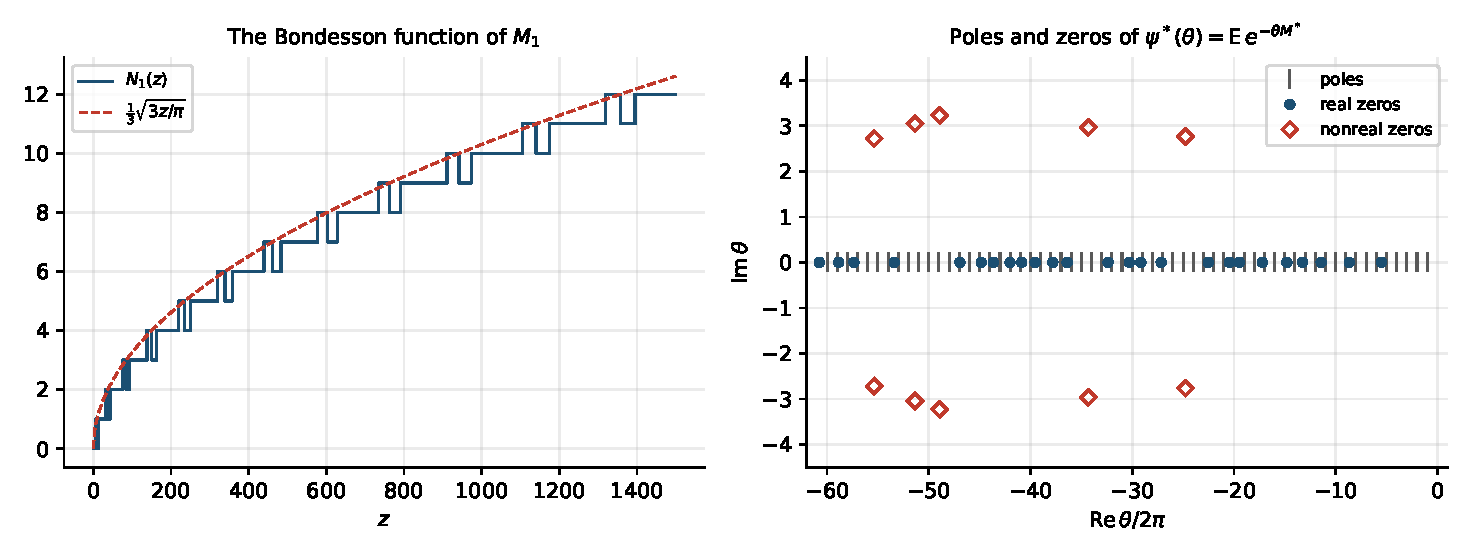
\includegraphics[width=\textwidth]{fig/maxexp_laws.pdf}
\caption{Left: the Bondesson function $N_1$ of $M_1$, nonnegative, with its asymptote $\frac13\sqrt{3z/\pi}$; each drop is a zero of the transform at $-b_{6k}$. Right: the poles $-2\pi m$, $m\le60$, and the zeros of $\psi^*(\theta)=\E e^{-\theta M^*}$: the $25$ real zeros above $-2\pi\times61$, one in each gap with $\tau(m+1)\tau(m+2)>0$, and the five pairs of nonreal zeros, the only ones with $|\re\theta|\le2\pi\times60.5$ and $|\im\theta|\le100$. Drawn by \texttt{maxexp\_figs.py} from \texttt{maxexp\_psizeros.json}.}
\label{fig:maxexp:laws}
\end{figure}

For the clock the relaxation from GGC to BO gains nothing. If its L\'evy density $W(t)/t$ were completely monotone, equal to $\int e^{-zt}\mu(dz)$ with $\mu\ge0$, then the formula $(G'/G)(u)=\int_0^\infty e^{-ut}W(t)\,dt$ of Section~\ref{ch:clock} would give $(G'/G)(u)=\int\mu(dz)(u+z)^{-2}$, holomorphic on $\cut$. But $G'/G$ has a pole at every zero $-a_k=(\rho_k-\frac12)^2$ of $G$, and this point lies in $(-\infty,0]$ only when $\rho_k$ is on the critical line. So the clock is in BO if and only if RH holds (Table~\ref{tab:ch3:hierarchy}). The signed Thorin measures of the max laws come from zeros of their Laplace transforms, and the transform $1/G$ of the clock has none. The two laws of this section show the two ways out of the Thorin class: $M_1$ leaves it through real zeros, each preceded by its own pole, and stays in BO, while $M^*$ leaves BO too, through zeros off the real axis, the way a zero of $\xi$ off the critical line would take the clock out of both classes.

Table~\ref{tab:maxexp:checks} collects the checks of this section, in the form of the table of the first author's note, recomputed.

\begin{table}[htbp]
\centering\small
\begin{tabular}{llp{0.24\textwidth}}
\toprule
quantity & max representation & check\\
\midrule
$L(\frac{17}2,\Delta)=\E\,Q(14,2\pi M^*)$ & $0.998583063162746176492$ & \raggedright Hecke: same; series to $n=400$: $18$ digits\tabularnewline
$L(\frac{29}2,\Delta)=\E\,Q(20,2\pi M^*)$ & $0.999977182799369841175$ & \raggedright series: same\tabularnewline
$\xi(\frac12,\Delta)$, symmetric form & $0.00154487936039502721$ & \raggedright \eqref{eq:ch16:max}, Hecke: same\tabularnewline
\eqref{eq:maxexp:fe}, $k=1$ & $0.00595896498957823785$ & \raggedright $k=11$: same\tabularnewline
\eqref{eq:maxexp:fe}, $k=5$ & $0.00163398603484069935$ & \raggedright $k=7$: same\tabularnewline
$L(\frac12,\Delta)=\Pr(N(2\pi M^*)\le5)$ & $0.792122838646030569$ & \raggedright Hecke: same\tabularnewline
first zero of $\xi(\frac12+i\theta,\Delta)$ & $9.2223793999211025222$ & \raggedright Hecke: same; \cite{LMFDB}: $9.222379$\tabularnewline
first zero of $K_{i\theta}(2\pi)$ & $9.768770083509977867$ & \raggedright moved to $9.2224$ by $H$\tabularnewline
$L(1,\chi_{12})$, $\operatorname{erfc}$ form & $0.760345996300946347531$ & \raggedright $\log(2+\sqrt3)/\sqrt3$: same\tabularnewline
$L(1,E)=\E e^{-2\pi M_{11}}$ & $0.253841860855910684338$ & \raggedright series of root number one: same\tabularnewline
$\E K$ from $\vartheta_4$ & $0.868731160636159141830$ & \raggedright $\sqrt{\pi/2}\,\log2$: same\tabularnewline
$\E e^{-2M_1}$, quadrature & $0.694250350153875231803$ & \raggedright closed form: same\tabularnewline
$\E e^{-3M_4}$, quadrature & $0.285645278943791835551$ & \raggedright $\sqrt{3\pi}/\sinh\sqrt{3\pi}$: same\tabularnewline
zeros of $\psi_1$ & $-b_{6k}=-\frac{36k^2-1}{12}\pi$ & \raggedright closed form vanishes at $k=1,2$\tabularnewline
$-\log|\E e^{5iM_1}|^2$ & $0.40295014525377167405$ & \raggedright Thorin sum: same; $\int N_1$: $18$ digits\tabularnewline
$-\psi_1'(2)/\psi_1(2)$ & $0.16796840787856222484$ & \raggedright Thorin sum: same; $\int N_1$: to $2\times10^{-15}$\tabularnewline
$-\log\psi_1(2)$ & $0.36492264843255339528$ & \raggedright L\'evy integral: same\tabularnewline
first zero of $\psi^*$ & $-2\pi\times5.48830041253$ & \raggedright certified; the only zero for $|\re\theta|\le15\pi$, $|\im\theta|\le60$ (computed)\tabularnewline
first nonreal zero of $\psi^*$ & $-155.59408228\pm2.76311889\,i$ & \raggedright certified\tabularnewline
\bottomrule
\end{tabular}
\caption[Checks of the max representation and of the laws of $M_1$ and $M^*$]{Checks of Section~\ref{sec:ch16:max}, by \texttt{maxlaw.py}, \texttt{maxexp\_checks.py} and \texttt{maxexp\_psizeros.py}, with $\psi_1(\theta)=\E e^{-\theta M_1}$; ``same'' means agreement to all digits shown. The first six rows are computed from the product for $F$ and the density \eqref{eq:maxexp:density}, independently of the Dirichlet series; the zeros of $\psi^*$ are those of Proposition~\ref{prop:maxexp:psizeros}.}
\label{tab:maxexp:checks}
\end{table}

\subsection{The de Bruijn Newman flow for \texorpdfstring{$\Delta$}{Delta}}\label{sec:ch16:dbn}

The flow of Section~\ref{ch:dbn} needs only an even kernel that decays faster than any Gaussian, so it applies to $K_\Delta$:
\[
H^\Delta_t(\theta)=\int_0^\infty e^{tu^2}K_\Delta(u)\cos(\theta u)\,du,\qquad 2H^\Delta_0(\theta)=\xi\big(\tfrac12+i\theta,\Delta\big).
\]
In the variable $\theta$ the times of Section~\ref{ch:dbn}, whose variable is $z=2\theta$, are divided by four, and the isolated pair estimate for two zeros at distance $D$ is $-D^2/8$. The zeros of $H^\Delta_0$ lie in the strip $|\im\theta|<\frac12$, so by de Bruijn's theorem \cite{deBruijn} every zero of $H^\Delta_t$ is real for $t\ge\frac18$; for $\zeta$ the same strip gives de Bruijn's bound $\Lambda\le\frac12$ in the times of Section~\ref{ch:dbn}. Dobner's theorem for the extended Selberg class \cite{Dobner21} gives the other side: $\Delta$ has a de Bruijn Newman constant $\Lambda_\Delta$, and $H^\Delta_t$ has nonreal zeros for every $t<0$. So $0\le\Lambda_\Delta\le\frac18$, and GRH for $\Delta$ is the statement $\Lambda_\Delta=0$.

On the critical line the kernel is a probability density up to normalisation, as the eta kernel is in Section~\ref{sec:ch16:eta}: if $V$ has the density $K_\Delta(v)/\xi(\frac12,\Delta)$ on $\R$, then $\E e^{i\theta V}=\xi(\frac12+i\theta,\Delta)/\xi(\frac12,\Delta)$, and GRH for $\Delta$ is the statement that this characteristic function has only real zeros. In the language of Section~\ref{sec:ch16:max}, $e^V$ has the density proportional to $y^5\Delta(iy)=y^5e^{-2\pi y}F(y)$, so $V$ is the logarithm of $G_6/2\pi$ conditioned on $G_6/2\pi\ge M^*$, with $G_6$ a gamma variable of shape $6$ independent of $M^*$; its law is symmetric by the self duality \eqref{eq:maxexp:dual}, with no symmetrisation. The variable $V$ is not infinitely divisible, nor even quasi infinitely divisible, because its characteristic function vanishes at $\theta=9.2223793999$; this is the argument of Proposition~\ref{sb:prop:qid}(1) for the P\'olya variable. Since $1-\cos x=2\sin^2(x/2)$ and $K_\Delta$ is even,
\[
\xi\big(\tfrac12,\Delta\big)-\xi\big(\tfrac12+i\theta,\Delta\big)=4\int_0^\infty K_\Delta(v)\sin^2\Big(\frac{\theta v}2\Big)dv,
\]
so the zeros on the critical line are the solutions of $\E[2\sin^2(\theta V/2)]=1$. At the level of logarithms, the factorisation $\xi(s,\Delta)=(2\pi)^{-s-11/2}\Gamma(s+\frac{11}2)L(s,\Delta)$ splits $\log|\xi(\frac12+i\theta,\Delta)/\xi(\frac12,\Delta)|^2$ into $\log|\Gamma(6+i\theta)/\Gamma(6)|^2$ and $\log|L(\frac12+i\theta,\Delta)/L(\frac12,\Delta)|^2$. The first has the positive sine squared form given by Binet's formula,
\[
\log\Big|\frac{\Gamma(6+i\theta)}{\Gamma(6)}\Big|^2=-\int_0^\infty4\sin^2\Big(\frac{\theta u}2\Big)\frac{e^{-6u}}{u(1-e^{-u})}\,du,
\]
the L\'evy Khintchine form of the infinitely divisible variable $\log G_6$, and the second carries every zero. To the right of the critical strip the second has a sine squared form too: for $\sigma>1$, expanding $\log L(s,f)=\sum_{n\ge2}\Lambda_f(n)n^{-s}/\log n$ gives
\[
\log\Big|\frac{L(\sigma+i\theta,f)}{L(\sigma,f)}\Big|^2=-\sum_{n\ge2}\frac{4\Lambda_f(n)}{n^\sigma\log n}\sin^2\Big(\frac{\theta\log n}2\Big),
\]
for $f=\chi_{12}$ and $\Delta$, and for $\zeta$ with $\Lambda$ in place of $\Lambda_f$. Since $\int_\sigma^\infty n^{-\alpha}d\alpha=n^{-\sigma}/\log n$, the right side is minus twice the integral of the prime piece of the decomposition of Section~\ref{sec:ch16:sin2} over the basepoints $\alpha>\sigma$. For $\zeta$ the weights are positive, which is the infinite divisibility of $\log$ of the zeta distribution (Section~\ref{rz:sec:strip}). For $\Delta$ they are $8\cos(k\vartheta_p)/(kp^{k\sigma})$ at $n=p^k$, where $\alpha_p=e^{i\vartheta_p}$, $0\le\vartheta_p\le\pi$, and they take both signs. The Sato Tate law for $\Delta$, proved by Barnet-Lamb, Geraghty, Harris and Taylor \cite{BLGHT11}, makes the angles $\vartheta_p$ equidistributed for the measure $\frac2\pi\sin^2\vartheta\,d\vartheta$ on $[0,\pi]$, under which $\cos k\vartheta<0$ with probability $\frac12$ for $k\ne2$ and $\frac12+\frac1\pi$ for $k=2$. So even where the Euler product converges absolutely the sine squared form of $\log|L(\sigma+i\theta,\Delta)|$ has a signed measure, and on the critical line the series diverges: positivity lives in the kernel and in the gamma factor, not in the arithmetic factor.

The kernel factors as $K_\Delta(u)=e^{-2\pi\cosh u}H(u)$, with $H(u)=\sqrt{F(e^u)F(e^{-u})}$ because $K_\Delta(u)^2=K_\Delta(u)K_\Delta(-u)$, and $\log H(u)=-12\sum_m\frac{\sigma(m)}m(e^{-2\pi me^u}+e^{-2\pi me^{-u}})$. The expansion comes from $-\log F(y)=24\sum_{m\ge1}\frac{\sigma(m)}me^{-2\pi my}$, so $-\log F$ is completely monotone, the Laplace transform of the positive measure with mass $24\sigma(m)/m$ at each point $2\pi m$; for $\eta$ the masses are $\sigma(m)/m$, and every maximum of independent exponential variables has this property, since $-\log(1-e^{-\lambda y})=\sum_ke^{-k\lambda y}/k$. The transform $K_{i\theta}(2\pi)$ of P\'olya's factor has only real zeros \cite{Polya}, the first at $\theta=9.768770083509977867$ (\texttt{maxlaw.py}), and the multiplier $H$ moves it to $9.2223793999$. P\'olya's theorem on universal factors \cite[p.~197]{deBruijn}, which covers the Gaussian multiplier $e^{tu^2}$ of the flow for $t>0$, does not apply to $H$, which is bounded by one and supplies half of the doubly exponential decay of $K_\Delta$. The positivity of the measure of $-\log F$ is automatic and does not by itself decide where the zeros are; whether some multiplier of the same form moves zeros off the line is the following question, and any answer must account for $\Delta$, $\chi_{12}$ and the conductor $11$ curve, whose kernels have this form. Figure~\ref{fig:maxexp:kernels} shows the two kernels and $\log H$.

\begin{question}\label{q:maxexp:mult}
For which $a>0$, $c_m\ge0$ and $\beta_m>0$ does the Fourier transform of $e^{-a\cosh u}\exp\big(-\sum_mc_m(e^{-\beta_me^u}+e^{-\beta_me^{-u}})\big)$ have only real zeros?
\end{question}

\begin{figure}[htbp]
\centering
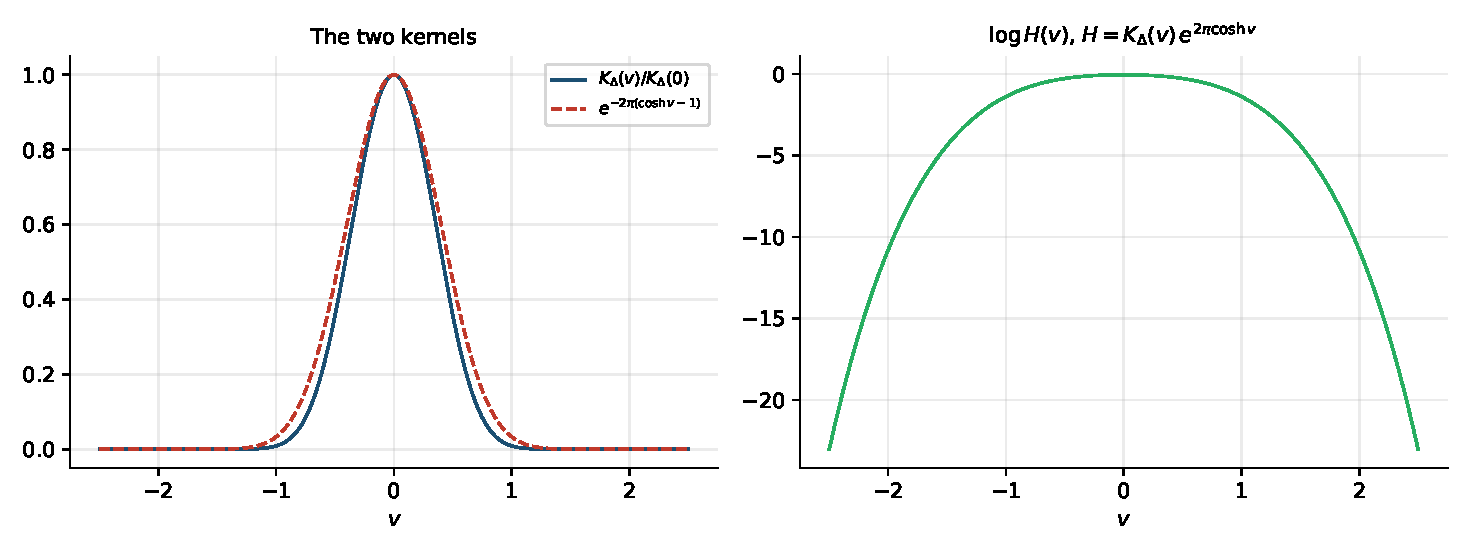
\includegraphics[width=\textwidth]{fig/maxexp_kernels.pdf}
\caption{Left: the kernel $K_\Delta(v)=e^{6v}\Delta(ie^v)$ and P\'olya's kernel $e^{-2\pi\cosh v}$, each divided by its value at $0$. Right: the logarithm of the multiplier $H(v)=\sqrt{F(e^v)F(e^{-v})}$; $-\log H$ expands with the positive coefficients $12\sigma(m)/m$. Drawn by \texttt{maxexp\_figs.py}.}
\label{fig:maxexp:kernels}
\end{figure}

The kernel $K_\Delta$ is strictly log concave, as the first author's note \cite{P26thor} shows, and the product formula gives the best constant. For $c>0$, $\log(1-e^{-ce^u})$ is the logarithm of the distribution function of $\log E$, with $E$ exponential of rate $c$, and it is strictly concave in $u$: with $x=ce^u$ its second derivative is $x(e^x-1-xe^x)/(e^x-1)^2<0$. So $\log F(e^u)$, a sum of such terms, is strictly concave (in the language of Section~\ref{sec:ch16:max}, $\log M^*$ has a log concave distribution function), and since $\log K_\Delta(u)=6u-2\pi e^u+\log F(e^u)$ and $K_\Delta$ is even,
\[
-\big(\log K_\Delta\big)''(u)>2\pi e^{|u|},\qquad u\in\R,
\]
where the ratio of the two sides tends to $1$ as $|u|\to\infty$. The multiplier $H$ is log concave as well, since $\log H(u)=\frac12\big(\log F(e^u)+\log F(e^{-u})\big)$. In the same way $\log K(u)=\log2+\frac u2-\frac\pi{12}e^{2u}+\log F_1(e^{2u})$ gives $-(\log K)''(u)>\frac\pi3e^{2|u|}$ for the kernel of Section~\ref{sec:ch16:eta}. The P\'olya kernel $\Phi$ is log concave too \cite{CC13}, though it is not a product of this kind. Log concavity alone does not put the zeros of a transform on a line, or in any strip. The function $(1-|u|)_+^2$ is log concave, and its transform $4(\theta-\sin\theta)/\theta^3$ vanishes at the nonzero roots of $\sin\theta=\theta$, which are nonreal, the first at $7.4977+2.7687i$, with imaginary parts that grow like $\log|\theta|$. Its convolution with $e^{-\cosh u}$ is even, positive, entire and log concave \cite{SW14}, and decays doubly exponentially, like $K_\Delta$; its transform $8(\theta-\sin\theta)K_{i\theta}(1)/\theta^3$ has the same nonreal zeros.

In the language of Section~\ref{sec:ch16:max} the flow is a family of Gaussian tilts: for every real $t$, $e^{tv^2}K_\Delta(v)$ is integrable, because $K_\Delta$ decays doubly exponentially, so after normalisation it is the density of the law of $V$ tilted by $e^{tV^2}$, and $H^\Delta_t(\theta)/H^\Delta_t(0)$ is its characteristic function. The question $\Lambda_\Delta=0$ asks whether the smallest tilt whose characteristic function has only real zeros is $t=0$.

The script \texttt{dbn\_delta.py} computes $H^\Delta_t$ by Gauss Legendre quadrature on $[0,4]$, beyond which $K_\Delta<10^{-130}$, with $8$ panels of $96$ nodes at $40$ digits; at $t=0$ it agrees with $192$ nodes per panel and with Hecke's formula to a relative $4\times10^{-41}$ at $\theta=0$ and $5\times10^{-16}$ at $\theta=50$. The $21$ zeros below height $52$, from $9.2224$ to $51.1566$, stay real for $t=0.05,0.1,\dots,0.5$ and all move down. Backward in time each pair of neighbours is followed through the critical point of $H^\Delta_t$ between them until the critical value changes sign, and each such event is tested by direct sign counts: a collision at $(t_*,\theta_*)$ leaves two sign changes on $[\theta_*-1.2,\theta_*+1.2]$ at $t_*+0.005$ and none at $t_*-0.005$, and the colliding pair is identified by the number of sign changes below $\theta_*-1.2$, since real zeros keep their order. Table~\ref{tab:ch16:coll} lists the seven collisions. The numbers of sign changes on $(0.5,52]$ at eleven values of $t$ from $0$ to $-1.5$ fall by two at each collision and once by one, between $t=-0.2$ and $-0.3$, where the highest zero, followed back from $51.1566$, passes $52$ at $t\approx-0.29$.

\begin{table}[htbp]
\centering\small
\begin{tabular}{cccc}
\toprule
pair at $t=0$ & $-D^2/8$ & $t_*$ & $\theta_*$\\
\midrule
$48.3591$, $49.2761$ & $-0.1051$ & $-0.12622$ & $49.18$\\
$36.7415$, $37.7539$ & $-0.1281$ & $-0.15864$ & $37.60$\\
$45.0401$, $46.1973$ & $-0.1674$ & $-0.24305$ & $46.19$\\
$25.2746$, $26.8044$ & $-0.2925$ & $-0.40713$ & $27.26$\\
$40.2190$, $41.7305$ & $-0.2856$ & $-0.48271$ & $42.49$\\
$31.1782$, $32.7749$ & $-0.3187$ & $-0.48637$ & $33.30$\\
$17.4428$, $19.6565$ & $-0.6126$ & $-0.98116$ & $21.09$\\
\bottomrule
\end{tabular}
\caption{The collisions of zeros of $H^\Delta_t$ below height $52$, in the order in which they occur as $t$ decreases: the pair at $t=0$, the isolated pair estimate with $D$ the gap of the pair, and the time $t_*$ and height $\theta_*$ of the collision, computed by \texttt{dbn\_delta.py}.}
\label{tab:ch16:coll}
\end{table}

The script \texttt{maxexp\_flow.py} recomputes the table independently, at $70$ digits for the kernel and with a different tracking: it evaluates $H^\Delta_t$ at once on the grid $\theta=0.5,0.52,\dots,52$, with the cosines kept in fixed point by their three term recurrence, for $t=0.5,0.49,\dots,-1.1$, locates the zeros by inverse interpolation, and refines each fall of the count by two to the time at which the critical value between the closest pair changes sign. It finds the same seven collisions, with the same $t_*$ and $\theta_*$ to all digits of the table (for instance $t_*=-0.4071263919$, $\theta_*=27.257965$), and the highest zero passing $52$ between $t=-0.29$ and $-0.30$. Figure~\ref{fig:maxexp:flow} shows the trajectories.

\begin{figure}[htbp]
\centering
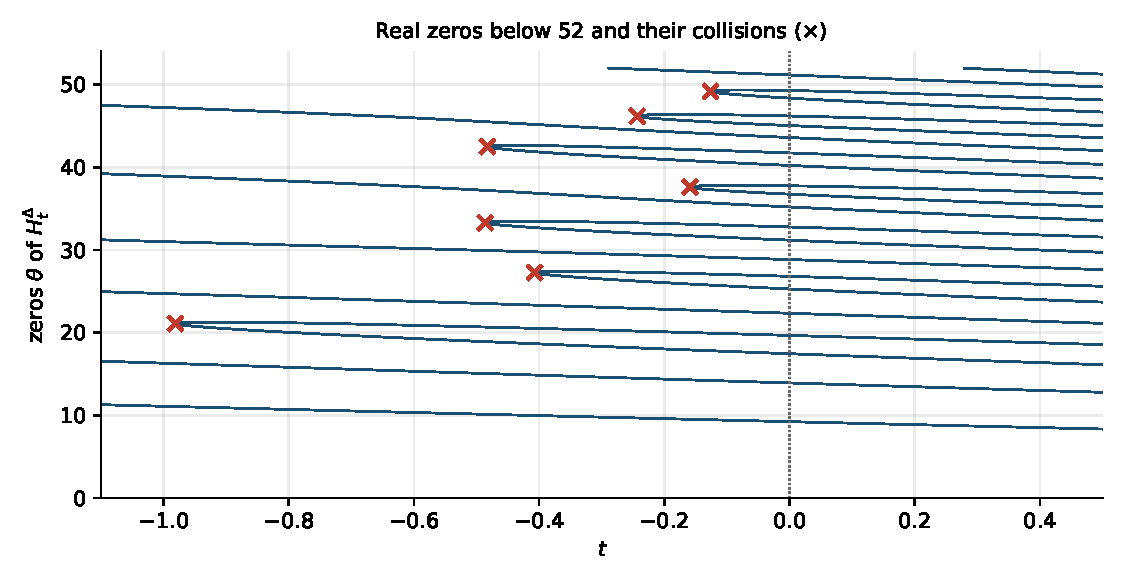
\includegraphics[width=0.8\textwidth]{fig/maxexp_flow.pdf}
\caption{The real zeros of $H^\Delta_t$ below height $52$ for $-1.1\le t\le0.5$, and the seven collisions of Table~\ref{tab:ch16:coll}; all zeros move down as $t$ grows. Drawn by \texttt{maxexp\_figs.py} from \texttt{maxexp\_flow.json}.}
\label{fig:maxexp:flow}
\end{figure}

The low zeros of $\Delta$ are robust: below height $33$, the window of the first author's note, the first pair to leave the line, $(25.27,26.80)$, does so only at $t=-0.407$. Collisions do not come in order of height, however. The pairs near $37.6$ and $49.2$ collide at $-0.159$ and $-0.126$, and under GRH for $\Delta$ Dobner's theorem forces collisions in every interval $(t,0)$, higher up; so no window of heights decides whether $\Lambda_\Delta=0$ (Dobner's theorem already gives $\Lambda_\Delta\ge0$), and what a computation can show is how fast the collision times approach $0$ with height. The neighbours delay every collision beyond the isolated pair estimate, by factors from $1.20$ to $1.69$. In the variable $\theta$ the closest pair of $\zeta$ below height $200$ collides at $-0.072$, and Lehmer's pair near height $7005$ at $-1.8\times10^{-4}$ (Section~\ref{sec:ch21:collisions}).

\subsection{A P\'olya kernel for imaginary quadratic fields}\label{sec:sqfree:quad}

Section~\ref{sec:ch16:eta} left the positivity of the kernels of odd characters to be checked case by case. For the Dedekind zeta function of an imaginary quadratic field the kernel comes from a simple theta series, its positivity reduces to a finite interval, and it fails for a whole residue class of discriminants, together with the kernel of the odd character. This subsection follows the last part of the first author's note on the squarefree series \cite{P26sqf}; the constants of number fields, which these kernels turn into tilted means, are in Section~\ref{sec:sqfree:nf} of Chapter~\ref{chap:strip}.

Let $d<0$ be a fundamental discriminant, $K=\mathbb Q(\sqrt d)$, $\chi_d$ the Kronecker symbol of $d$, a real primitive odd character modulo $|d|$, $h$ the class number of $K$ and $w$ the number of its roots of unity. Then $\zeta_K(s)=\zeta(s)L(s,\chi_d)=\sum_{n\ge1}a_nn^{-s}$, where $a_n=\sum_{m\mid n}\chi_d(m)\ge0$ is the number of ideals of norm $n$, and we put
\[
\Lambda_K(s)=\Big(\frac{\sqrt{|d|}}{2\pi}\Big)^s\Gamma(s)\,\zeta_K(s),\qquad \xi_K(s)=2s(s-1)\Lambda_K(s),
\]
the function $\xi_K$ of Section~\ref{sec:sqfree:nf} with $r_1=0$ and $r_2=1$. The duplication formula gives $\xi_K(s)=\frac2{\sqrt{|d|}}\,\xi(s)\,\xi(s,\chi_d)$, with $\xi(s,\chi_d)=(|d|/\pi)^{(s+1)/2}\Gamma(\frac{s+1}2)L(s,\chi_d)$ the completed function of Section~\ref{sec:ch16:eta}, so $\xi_K(s)=\xi_K(1-s)$ because the root number of $\chi_d$ is one. Hence $\Lambda_K(s)=\Lambda_K(1-s)$, and $\Lambda_K$ is meromorphic with simple poles at $s=1$ and $s=0$ only, with residues $h/w$ and $-h/w$, by the class number formula $L(1,\chi_d)=2\pi h/(w\sqrt{|d|})$ and the symmetry. Let
\[
\vartheta_K(x)=\sum_{n\ge1}a_n\,e^{-2\pi nx/\sqrt{|d|}},\qquad \Psi(y)=y(y-2)\,e^{-y},\qquad H_K(x)=\big(x^2\vartheta_K'(x)\big)',
\]
and $\Phi_K(u)=2e^{u/2}H_K(e^u)$.

\begin{theorem}\label{thm:sqfree:kernelK}
\textup{(i)} $\vartheta_K(1/x)=x\,\vartheta_K(x)+\frac hw\,(x-1)$ for $x>0$.

\textup{(ii)} $H_K(x)=\sum_{n\ge1}a_n\Psi(2\pi nx/\sqrt{|d|})$ and $H_K(1/x)=x\,H_K(x)$. The kernel $\Phi_K$ is even, analytic in the strip $|\im u|<\frac\pi2$, and decays doubly exponentially.

\textup{(iii)} $\xi_K(\frac12+s)=\int_{\R}\Phi_K(u)\,e^{su}\,du$ for every $s\in\C$; in particular $\xi_K(\frac12+i\theta)=\int_{\R}\Phi_K(u)\cos(\theta u)\,du$.

\textup{(iv)} $\Phi_K>0$ on $\R$ if and only if $H_K>0$ on $[1,\sqrt{|d|}/\pi]$. In particular $\Phi_K>0$ when $|d|<\pi^2$, that is for $d=-3,-4,-7,-8$.

\textup{(v)} If $\Phi_K>0$, then $\zeta_K(\frac12)<0$ and $L(\frac12,\chi_d)>0$. In particular $L(\frac12,\chi_d)>0$ for $d=-3,-4,-7,-8$.
\end{theorem}

\begin{proof}
(i) For $c>1$, Mellin inversion of $\int_0^\infty e^{-2\pi nx/\sqrt{|d|}}x^{s-1}dx=\Gamma(s)\big(\sqrt{|d|}/2\pi n\big)^s$ gives $\vartheta_K(x)=\frac1{2\pi i}\int_{(c)}\Lambda_K(s)x^{-s}ds$. Move the line of integration to $\re s=1-c$, which the exponential decay of $\Gamma$ and the polynomial growth of $\zeta_K$ on vertical strips allow; the residues at $s=1$ and $s=0$ are $\frac hwx^{-1}$ and $-\frac hw$. On the new line substitute $s\mapsto1-s$ and use $\Lambda_K(1-s)=\Lambda_K(s)$: the integral becomes $x^{-1}\vartheta_K(1/x)$. So $\vartheta_K(x)=\frac hw(x^{-1}-1)+x^{-1}\vartheta_K(1/x)$, which is (i).

(ii) Termwise, $\big(x^2\frac d{dx}e^{-\kappa x}\big)'=(\kappa^2x^2-2\kappa x)e^{-\kappa x}=\Psi(\kappa x)$. Differentiating (i) gives $\vartheta_K'(1/x)=-x^2\big(\vartheta_K(x)+x\vartheta_K'(x)+\frac hw\big)$, so $g(x)=x^2\vartheta_K'(x)$ satisfies $g(1/x)=-\big(\vartheta_K(x)+x\vartheta_K'(x)+\frac hw\big)$, and differentiating again gives $g'(1/x)=x^2\big(2\vartheta_K'(x)+x\vartheta_K''(x)\big)=x\,g'(x)$, that is $H_K(1/x)=xH_K(x)$. Then $\Phi_K(-u)=2e^{-u/2}H_K(e^{-u})=2e^{u/2}H_K(e^u)=\Phi_K(u)$. Since $a_n\le n$, the series for $H_K(e^u)$ converges locally uniformly where $\re e^u>0$, that is for $|\im u|<\frac\pi2$; and $\Phi_K(u)=O\big(e^{5u/2}\exp(-2\pi e^u/\sqrt{|d|})\big)$ as $u\to\infty$, and likewise as $u\to-\infty$ by evenness.

(iii) By (i), $x\vartheta_K(x)\to\frac hw$ and $x^2\vartheta_K'(x)\to-\frac hw$ as $x\to0$, while $\vartheta_K$ and $\vartheta_K'$ decay exponentially at infinity. For $\re z>1$ two integrations by parts, whose boundary terms vanish, give $\int_0^\infty H_K(x)x^{z-1}dx=z(z-1)\int_0^\infty\vartheta_K(x)x^{z-1}dx=z(z-1)\Lambda_K(z)$. With $x=e^u$ and $z=\frac12+s$, $\int_{\R}\Phi_K(u)e^{su}du=2\int_0^\infty H_K(x)x^{z-1}dx=\xi_K(z)$. Both sides are entire in $s$, the left by (ii), so the identity holds for every $s$.

(iv) By (ii), $\Phi_K>0$ exactly when $H_K>0$ on $(0,\infty)$, and by the symmetry exactly when $H_K>0$ on $[1,\infty)$. For $x\ge\sqrt{|d|}/\pi$ every argument $2\pi nx/\sqrt{|d|}$ is at least $2n\ge2$, where $\Psi\ge0$, and the term $n=4$ is positive, since $a_4=1+\chi_d(2)+\chi_d(2)^2\ge1$; so $H_K>0$ there. If $|d|<\pi^2$ the interval $[1,\sqrt{|d|}/\pi]$ is empty.

(v) By (iii), $\xi_K(\frac12)=\int_{\R}\Phi_K>0$, while
\[
\xi_K\big(\tfrac12\big)=-\tfrac12\Lambda_K\big(\tfrac12\big)=-\tfrac12\big(\sqrt{|d|}/2\pi\big)^{1/2}\sqrt\pi\,\zeta_K\big(\tfrac12\big).
\]
So $\zeta_K(\frac12)<0$, and $L(\frac12,\chi_d)=\zeta_K(\frac12)/\zeta(\frac12)>0$ because $\zeta(\frac12)<0$.
\end{proof}

When $\Phi_K>0$, the normalised kernel $\Phi_K/\xi_K(\frac12)$ is the density of a symmetric variable $X_K$ with $\E e^{sX_K}=\xi_K(\frac12+s)/\xi_K(\frac12)$, the P\'olya variable of $K$, and its tilts $V_{K,\alpha}$, with $\E e^{sV_{K,\alpha}}=\xi_K(\alpha+s)/\xi_K(\alpha)$, have the means $\frac{\xi_K'}{\xi_K}(\alpha)$. The zero part of the constant $C_K$ of Theorem~\ref{thm:sqfree:constK} is then $\E V_{K,1}-2\,\E V_{K,2}$, as over $\mathbb Q$ in Theorem~\ref{thm:sqfree:const}; by (iv) this applies to the Gaussian field $d=-4$ of Section~\ref{sec:sqfree:nf}. If moreover the Riemann hypothesis holds for $\zeta_K$, that is RH for $\zeta$ and for $L(s,\chi_d)$, then $1/\E\cosh(\sqrt u\,X_K)=\xi_K(\frac12)/\xi_K(\frac12+\sqrt u)$ is the Laplace transform of a GGC, the clock of $K$ (Proposition~\ref{prop:sqfree:thorinK}).

The kernel $\Phi_K$ is tied to the kernel of $\chi_d$ in Section~\ref{sec:ch16:eta},
\[
K_{\chi_d}(u)=2e^{3u/2}\sum_{n\ge1}n\chi_d(n)\,e^{-\pi n^2e^{2u}/|d|},\qquad \xi\big(\tfrac12+s,\chi_d\big)=\int_{\R}K_{\chi_d}(u)\,e^{su}\,du .
\]
Since the two sided Laplace transform turns convolution into multiplication, the identity $\xi_K=\frac2{\sqrt{|d|}}\xi\cdot\xi(\cdot,\chi_d)$ and (iii) give $\Phi_K=\frac2{\sqrt{|d|}}\,\Phi*K_{\chi_d}$, with $\Phi$ the P\'olya kernel \eqref{eq:ch2:Phi}. As $\Phi>0$, the kernel $\Phi_K$ is positive whenever $K_{\chi_d}$ is, and if $\Phi_K$ takes a negative value, so does $K_{\chi_d}$. For $d=-4$ Jacobi's identity $\sum_{n\ge0}(-1)^n(2n+1)q^{(2n+1)^2/8}=q^{1/8}\prod_{n\ge1}(1-q^n)^3$ gives $K_{\chi_{-4}}(u)=2e^{3u/2}\eta(ie^{2u})^3>0$, positive by the product formula as the kernel of $\chi_{12}$ is.

The script \texttt{sqfree\_quadratic.py} checks the theorem at $30$ digits. For $d=-4$, where $h/w=\frac14$, the trapezoid rule with step $1/200$ gives $\int\Phi_K(u)\cos(\theta u)\,du=0.48753311500024448536$ at $\theta=0$ and $0.25376667901239784985$ at $\theta=2.5$, equal to $\xi_K(\frac12+i\theta)$ in every digit shown; (i) holds at $x=1.5$ and $2$, and the evenness of $\Phi_K$ at $u=0.3$ and $0.6$, within $10^{-31}$; and $H_K(1/x)=xH_K(x)$ holds at $x=1.25$ within $3\times10^{-31}$ for $d=-23$ and $d=-163$, where $H_K(1.25)=0.55669258$ and $-0.28242077$. The values $\zeta_K(\frac12)=-0.70223711$, $-0.97506623$, $-1.6744215$ and $-1.6070054$ for $d=-3,-4,-7,-8$ are negative, as (v) requires.

Since $\int_0^\infty\Psi(y)\,dy=0$, the value $H_K(1)=\sum_na_n\Psi(2\pi n/\sqrt{|d|})$ is a Riemann sum, with step $2\pi/\sqrt{|d|}$ and weights $a_n$ of mean value $L(1,\chi_d)$, of a function with integral zero. For large $|d|$ it is small compared with the sum of the absolute values of its terms, and its sign, like the sign of $H_K$ elsewhere on $[1,\sqrt{|d|}/\pi]$, depends strongly on the first few weights: $\Psi$ is negative on $(0,2)$ and positive beyond, and the weights $a_2=1+\chi_d(2)$ and $a_3=1+\chi_d(3)$ vanish when $2$ and $3$ are inert in $K$. The next theorem makes this precise at the point where the term $n=1$ sits in the negative part of $\Psi$ and the terms $n=2$ and $3$, which would compensate it, vanish.

\begin{theorem}\label{thm:sqfree:inert}
Let $d<0$ be a fundamental discriminant with $\chi_d(2)=\chi_d(3)=-1$, that is $d\equiv5\pmod{24}$. Then $H_K(x)<0$ at $x=1.42\sqrt{|d|}/2\pi$, so $\Phi_K$ takes negative values, and so does the kernel $K_{\chi_d}$. There are infinitely many such $d$, for instance $d=-p$ for every prime $p\equiv19\pmod{24}$.
\end{theorem}

\begin{proof}
For a fundamental discriminant $d<0$, $\chi_d(2)=-1$ exactly when $d\equiv5\pmod8$, and $\chi_d(3)=-1$ exactly when $d\equiv2\pmod3$; together they give $d\equiv5\pmod{24}$. The function $n\mapsto a_n$ is multiplicative, with $a_{p^k}=\frac12(1+(-1)^k)$ when $\chi_d(p)=-1$ and $a_{p^k}\le k+1$ for every $p$. Hence $a_1=1$, $a_2=a_3=0$ and $a_n\le a_n^*$, where $a_n^*=0$ unless $2$ and $3$ divide $n$ to even powers, and otherwise $a_n^*$ is the number of divisors of $n$ with its factors $2$ and $3$ removed. At $x=1.42\sqrt{|d|}/2\pi$ the $n$th argument of $\Psi$ in Theorem~\ref{thm:sqfree:kernelK}(ii) is $1.42n$, which exceeds $2$ for $n\ge2$, where $\Psi>0$. So
\begin{align*}
H_K(x)&\le\Psi(1.42)+\sum_{n\ge4}a_n^*\,\Psi(1.42n)\\
&=-0.19907566+0.13917904=-0.05989662<0,
\end{align*}
the sum taken to $n=2000$ and the rest bounded, with $a_n^*\le2\sqrt n$, by $10^{-1225}$ (\texttt{sqfree\_quadratic.py}). Then $\Phi_K(\log x)<0$, and $K_{\chi_d}$ takes negative values by the convolution identity above. If $p\equiv19\pmod{24}$ is prime, then $p\equiv3\pmod4$, so $-p$ is a fundamental discriminant, and $-p\equiv5\pmod{24}$; by Dirichlet's theorem there are infinitely many such primes.
\end{proof}

The bound is negative for every $y$ in $[1.107,1.879]$ on a grid of step $0.001$, with least value $-0.0598979$ at $y=1.418$, so the point $x=y\sqrt{|d|}/2\pi$ can be moved. By the symmetry $H_K(1/x)=xH_K(x)$ it does not matter whether $x$ lies in $[1,\sqrt{|d|}/\pi]$; for $d=-19$ it does not.

Table~\ref{tab:sqfree:named} shows the discriminants discussed in the first author's note. The four of class number one with $2$ and $3$ inert, $d=-19,-43,-67,-163$, take the least value of $H_K$ on $[1,\sqrt{|d|}/\pi]$ at the centre $x=1$, the two composite ones with $d\equiv5\pmod{24}$ inside the interval, and most of the positive kernels at its right end $\sqrt{|d|}/\pi$, where the term $n=1$ vanishes. All twenty values of $\zeta_K(\frac12)$ computed are negative, so $L(\frac12,\chi_d)>0$ for all of them whether or not the kernel is positive: Theorem~\ref{thm:sqfree:kernelK}(v) is a sufficient condition only.

\begin{table}[htbp]
\centering\small
\begin{tabular}{rrrcrrr}
\toprule
$d$ & $\chi_d(2)$ & $\chi_d(3)$ & $\Phi_K>0$ & least $H_K$ on $[1,\sqrt{|d|}/\pi]$ & at $x=$ & $\zeta_K(\frac12)$\\
\midrule
$-11$ & $-1$ & $1$ & yes & $0.14236$ & $1.0557$ & $-1.4480539$\\
$-15$ & $1$ & $0$ & yes & $0.40606$ & $1.2328$ & $-2.6973176$\\
$-20$ & $0$ & $1$ & yes & $0.287033$ & $1.4235$ & $-2.4529153$\\
$-23$ & $1$ & $1$ & yes & $0.4634$ & $1.5266$ & $-3.5856997$\\
$-24$ & $0$ & $0$ & yes & $0.225215$ & $1.2409$ & $-2.2955534$\\
$-31$ & $1$ & $-1$ & yes & $0.349008$ & $1.7723$ & $-3.2253855$\\
$-39$ & $1$ & $0$ & yes & $0.409694$ & $1.9878$ & $-4.0547932$\\
$-47$ & $1$ & $1$ & yes & $0.46368$ & $2.1822$ & $-4.8243519$\\
$-71$ & $1$ & $1$ & yes & $0.470667$ & $2.6821$ & $-5.9925928$\\
$-191$ & $1$ & $1$ & yes & $0.470667$ & $4.3991$ & $-8.1483722$\\
$-19$ & $-1$ & $-1$ & no & $-0.0596605$ & $1$ & $-1.1747378$\\
$-43$ & $-1$ & $-1$ & no & $-0.214707$ & $1$ & $-0.76635571$\\
$-67$ & $-1$ & $-1$ & no & $-0.251274$ & $1$ & $-0.54460945$\\
$-163$ & $-1$ & $-1$ & no & $-0.315818$ & $1$ & $-0.10008066$\\
$-427$ & $-1$ & $-1$ & no & $-0.181949$ & $3.1887$ & $-0.20993694$\\
$-1003$ & $-1$ & $-1$ & no & $-0.228309$ & $3.9479$ & $-0.64248774$\\
\bottomrule
\end{tabular}
\caption{The P\'olya kernel $\Phi_K$ of $K=\mathbb Q(\sqrt d)$ for the discriminants named in the first author's note: the characters at $2$ and $3$, the sign of the kernel, the least value of $H_K$ on $[1,\sqrt{|d|}/\pi]$, which decides it by Theorem~\ref{thm:sqfree:kernelK}(iv), with the point where it is attained, and $\zeta_K(\frac12)=\zeta(\frac12)L(\frac12,\chi_d)$. Computed by \texttt{sqfree\_quadratic.py}.}
\label{tab:sqfree:named}
\end{table}

The script also scans all $6079$ fundamental discriminants $-20000\le d<0$. It evaluates $H_K$ in double precision on $3000$ geometrically spaced points of $[1,\sqrt{|d|}/\pi]$, refines the least value by golden section search, and would recompute at $30$ digits any least value within $10^{-8}$ of zero; there is none. The kernel is positive for $2738$ of the discriminants. Table~\ref{tab:sqfree:quad} sorts them by the splitting of $2$ and $3$: the proportion of positive kernels falls as either prime goes from split to ramified to inert, and the class $d\equiv5\pmod{24}$ of Theorem~\ref{thm:sqfree:inert} has none among its $763$ members. By blocks of $2000$ in $|d|$ the proportion falls from $337/611$ for $|d|\le2000$ to between $0.41$ and $0.45$ in each of the five blocks above $10000$. Of the $3341$ negative kernels, $1546$ take the least value of $H_K$ on $[1,\sqrt{|d|}/\pi]$ at the centre $x=1$, and $1135$ the least value of $\Phi_K$ on $u\ge0$ at $u=0$.

\begin{table}[htbp]
\centering\small
\begin{tabular}{lccc}
\toprule
 & $\chi_d(3)=1$ & $\chi_d(3)=0$ & $\chi_d(3)=-1$\\
\midrule
$\chi_d(2)=1$ & $676/767$ & $334/507$ & $412/757$\\
$\chi_d(2)=0$ & $489/753$ & $178/514$ & $131/757$\\
$\chi_d(2)=-1$ & $397/761$ & $121/500$ & $0/763$\\
\bottomrule
\end{tabular}
\caption{Positive P\'olya kernels $\Phi_K$ among the $6079$ fundamental discriminants $-20000\le d<0$, by the splitting of $2$ and $3$ in $K=\mathbb Q(\sqrt d)$ ($\chi_d(p)=1$ split, $0$ ramified, $-1$ inert): the number of positive kernels over the number of discriminants in each class, $2738$ positive in all. The empty corner is Theorem~\ref{thm:sqfree:inert}. Computed by \texttt{sqfree\_quadratic.py}.}
\label{tab:sqfree:quad}
\end{table}

\begin{question}\label{q:sqfree:density}
Does the proportion of fundamental discriminants $-X\le d<0$ with $\Phi_K>0$ tend to a limit as $X\to\infty$, and is the limit positive? Is $\Phi_K$ positive for infinitely many $d$, for instance among the $d$ in which $2$ and $3$ split, where the proportion up to $20000$ is $676/767$?
\end{question}

\begin{question}\label{q:sqfree:realquad}
For real quadratic fields and for fields of higher degree the gamma factor $\Gamma_{\mathbb R}(s)^{r_1}\Gamma_{\mathbb C}(s)^{r_2}$ replaces the exponentials in $\vartheta_K$ by other kernels, for $\Gamma_{\mathbb R}(s)^2$ a Bessel function $K_0$. Is there a criterion for the positivity of the P\'olya kernel of $\xi_K$ as simple as Theorem~\ref{thm:sqfree:kernelK}(iv)?
\end{question}

\subsection{The Dirichlet beta function and the eta cube kernel}\label{sec:dbeta:beta}

The $L$ function of the odd character $\chi_4$ modulo $4$, with $\chi_4(n)=1$ for $n\equiv1$, $-1$ for $n\equiv3\pmod4$ and $0$ for even $n$,
\[
L(s,\chi_4)=\sum_{n\ge0}\frac{(-1)^n}{(2n+1)^s}=\prod_p\big(1-\chi_4(p)p^{-s}\big)^{-1},\qquad\re s>1,
\]
is the Dirichlet beta function, with $L(1,\chi_4)=\frac\pi4$ and $L(2,\chi_4)$ Catalan's constant. It is the character $\chi_{-4}$ of Section~\ref{sec:sqfree:quad}, whose kernel is the cube of the Dedekind eta function and positive by the product formula. This subsection carries the Thorin framework over to it, following the first author's note \cite{P26beta}. Against $\zeta$ two things change, as for $\chi_{12}$: there is no pole, and the prime weights $\chi_4(n)\Lambda(n)$ take both signs, negative at the primes $3,7,11,19,\dots$. Against $\chi_{12}$ one thing changes: the character is odd, so the gamma factor is $\Gamma(\frac{s+1}2)$, and the archimedean piece of the sine squared decomposition is that of $\xi$ at the basepoint one lower. Section~\ref{sec:dbeta:kernel} gives the kernel, its reading as a Brownian exit time and the zeros below height $100$; Section~\ref{sec:dbeta:levy} the L\'evy form, the sine squared decomposition, and the exact range of basepoints where bounding the prime weights by their absolute values suffices; Section~\ref{sec:dbeta:qi} the factorisation through the Gaussian field $\mathbb Q(i)$, which writes the Thorin density as a difference of two Thorin densities; Section~\ref{sec:dbeta:arg} the Thorin measure on a vertical line as the argument of the completed function; and Section~\ref{sec:dbeta:centre} what transfers to the centre. The comparison across vertical lines of the note, which applies to $\xi$ and $L(s,\chi_{12})$ as well, is in Section~\ref{sec:dbeta:comp}.

\subsubsection{The kernel, the exit time and the zeros}\label{sec:dbeta:kernel}

Jacobi's identity $\eta(\tau)^3=q^{1/8}\prod_{m\ge1}(1-q^m)^3=\sum_{n\ge0}(-1)^n(2n+1)q^{(2n+1)^2/8}$, with $q=e^{2\pi i\tau}$ (Section~\ref{sec:sqfree:quad}), gives at $\tau=ix$ the theta series of $\chi_4$,
\[
\eta(ix)^3=\sum_{n\ge1}\chi_4(n)\,n\,e^{-\pi n^2x/4}=e^{-\pi x/4}\prod_{m\ge1}\big(1-e^{-2\pi mx}\big)^3,\qquad x>0,
\]
and the transformation $\eta(i/x)=\sqrt x\,\eta(ix)$ gives $\eta(i/x)^3=x^{3/2}\eta(ix)^3$. In the normalisation of Section~\ref{sec:ch16:eta} for odd characters the completed function is
\[
\xi(s,\chi_4)=\Big(\frac4\pi\Big)^{(s+1)/2}\Gamma\Big(\frac{s+1}2\Big)L(s,\chi_4)=\int_0^\infty\eta(ix)^3\,x^{(s+1)/2}\,\frac{dx}x,
\]
the integral by termwise integration for $\re s>1$, since $\int_0^\infty e^{-\pi n^2x/4}x^{(s+1)/2-1}dx=\Gamma(\frac{s+1}2)(4/\pi n^2)^{(s+1)/2}$, and for every $s$ by analytic continuation, since $\eta(ix)^3$ decays like $e^{-\pi x/4}$ as $x\to\infty$ and, by the transformation, like $x^{-3/2}e^{-\pi/(4x)}$ as $x\to0$. The transformation gives $\xi(s,\chi_4)=\xi(1-s,\chi_4)$, the root number of $\chi_4$ being one, and $\xi(s,\chi_4)$ is entire of order one, with no factor $s(s-1)$ to remove. It is $2/\sqrt\pi$ times the function $\Lambda$ of \cite{P26beta}, and $\xi(1,\chi_4)=\frac4\pi L(1,\chi_4)=1$. Section~\ref{sec:sqfree:quad} notes that the kernel of $\xi(s,\chi_4)$ is positive by the product formula; the next proposition collects its properties.

\begin{proposition}\label{prop:dbeta:kernel}
The kernel $K_4(u)=2e^{3u/2}\eta(ie^{2u})^3$ satisfies $\xi(\frac12+s,\chi_4)=\int_{\R}K_4(u)\,e^{su}\,du$ for every complex $s$. It is even, positive and analytic in the strip $|\im u|<\pi/4$, it has the symmetric product form
\[
K_4(u)=2\exp\Big(-\frac\pi4\cosh2u\Big)\prod_{m\ge1}\big(1-e^{-2\pi me^{2u}}\big)^{3/2}\big(1-e^{-2\pi me^{-2u}}\big)^{3/2},
\]
so that $K_4(u)=2\exp\big(\frac32|u|-\frac\pi4e^{2|u|}\big)\big(1+O(e^{-2\pi e^{2|u|}})\big)$, and $K_4(0)=2\eta(i)^3=\Gamma(\frac14)^3/(4\pi^{9/4})=0.906767655167731$.
\end{proposition}

\begin{proof}
With $x=e^{2u}$, $x^{(s+1)/2}dx/x=2e^{(s+1)u}du$, so the Mellin form with $\frac12+s$ in place of $s$ is the stated integral. The product formula makes every factor of $K_4(u)=2e^{3u/2}e^{-\frac\pi4e^{2u}}\prod_m(1-e^{-2\pi me^{2u}})^3$ positive. The transformation gives $K_4(-u)=2e^{-3u/2}\eta(ie^{-2u})^3=2e^{-3u/2}e^{3u}\eta(ie^{2u})^3=K_4(u)$. Hence $K_4(u)=\sqrt{K_4(u)K_4(-u)}$, and in the product $K_4(u)K_4(-u)$ the factors $e^{\pm3u/2}$ cancel while $e^{-\frac\pi4(e^{2u}+e^{-2u})}=e^{-\frac\pi2\cosh2u}$, which gives the symmetric form. For $u\to+\infty$ the product for $K_4(u)$ itself gives the asymptotic, and evenness gives it for $u\to-\infty$. The function $\eta(ie^{2u})$ is analytic where $\re e^{2u}>0$, that is for $|\im u|<\pi/4$. Finally $\eta(i)=\Gamma(\frac14)/(2\pi^{3/4})$.
\end{proof}

Like the kernel $K$ of $L(s,\chi_{12})$, $K_4$ is analytic in the same strip as the P\'olya kernel and decays doubly exponentially, so the evaluator of Section~\ref{ch:polya} applies unchanged. The script \texttt{dbeta\_thorin.py} computes $\xi(\frac12+s,\chi_4)$ from $K_4$ by the trapezoid rule with step $1/64$ on $|u|\le3$ and agrees with the Dirichlet $L$ function of Arb \cite{Arb} in all fourteen digits printed at $s=0$, $\frac12$, $0.1+5i$ and $0.1+20i$; for instance $\xi(\frac12,\chi_4)=0.98071361405771$, $\xi(0.6+5i,\chi_4)=0.080871220951695+0.011736751015145i$ and $\xi(0.6+20i,\chi_4)=(-2.3183027026127-0.20613003173368i)\times10^{-6}$. Also $L(\frac12,\chi_4)=0.667691457189609$.

\begin{remark}[The exit time]\label{rem:dbeta:exit}
By Theorem~\ref{bs:thm:eta}, $\frac4\pi\eta(4it/\pi)^3$ is the density of $X_C=\sum_ke_k/(2k-1)^2$, which is $\frac{\pi^2}8$ times the exit time $\tau$ of Brownian motion from $(-1,1)$ (Section~\ref{bh:sec:dict}). With $x=4t/\pi$, $\eta(ix)^3$ is therefore the density on $(0,\infty)$ of $Z=\frac4\pi X_C=\frac\pi2\tau$ \cite[Section 3]{P26thor}, and
\[
\xi(s,\chi_4)=\E\big[Z^{(s-1)/2}\big],\qquad \E e^{-uZ}=\sech\sqrt{\pi u}=\prod_{k\ge1}\Big(1+\frac{4u}{\pi(2k-1)^2}\Big)^{-1}.
\]
So $Z$ is a GGC with Thorin measure $\sum_k\delta_{\pi(2k-1)^2/4}$; its total mass $\xi(1,\chi_4)=1$ is the value $L(1,\chi_4)=\frac\pi4$, and its mean $\xi(3,\chi_4)=\frac4\pi\sum_k(2k-1)^{-2}=\frac\pi2$ is the value $L(3,\chi_4)=\pi^3/32$. The transformation $\eta(i/x)^3=x^{3/2}\eta(ix)^3$ says that $1/Z$ has the density $x^{-2}\eta(i/x)^3=x^{-1/2}\eta(ix)^3$, that is $\E g(1/Z)=\E[Z^{-1/2}g(Z)]$ for $g\ge0$, and with $g(z)=z^{(1-s)/2}$ this is the functional equation. The primal variable $Y_4$, with density $K_4/\xi(\frac12,\chi_4)$ and $\E e^{sY_4}=\xi(\frac12+s,\chi_4)/\xi(\frac12,\chi_4)$, is $\frac12\log Z$ under the size biasing by $Z^{-1/4}$, since $\E[Z^{-1/4}e^{(s/2)\log Z}]/\E[Z^{-1/4}]=\E[Z^{s/2-1/4}]/\E[Z^{-1/4}]$. So the analogue of the P\'olya variable is half the logarithm of a Brownian exit time biased by $Z^{-1/4}$, as for $\zeta$ it is half the logarithm of the variable $\pi S_2/2$ of Williams and of Biane, Pitman and Yor biased by $(\pi S_2/2)^{1/4}$ (Section~\ref{sec:ch19:williams}). In the notation of Section~\ref{pk:sec:theta}, $Z=1/\mathcal B_{\chi_{-4}}$ (Proposition~\ref{pk:prop:reflected}); whether $1/Z$ is a GGC is open, though it passes the test of that section to order $12$, and HCM cannot decide it, since the density of $Z$ is not HCM by Theorem~\ref{bs:thm:eta}. The script checks $\int_0^\infty\eta(ix)^3dx=1$ and $\int_0^\infty e^{-x}\eta(ix)^3dx=\sech\sqrt\pi=0.33029501666335$ to fourteen digits.
\end{remark}

The basepoint one has an explicit drift. By the functional equation $b_1=\frac{\xi'}\xi(1,\chi_4)=-\frac{\xi'}\xi(0,\chi_4)$. With $L(s,\chi_4)=4^{-s}\big(\zeta(s,\frac14)-\zeta(s,\frac34)\big)$, $\zeta(0,a)=\frac12-a$ and Lerch's formula $\partial_s\zeta(0,a)=\log\Gamma(a)-\frac12\log2\pi$ \cite[\S25.11]{DLMF}, one has $L(0,\chi_4)=\frac12$ and $L'(0,\chi_4)=\log\big(\Gamma(\frac14)/2\Gamma(\frac34)\big)$, and with $\psi(\frac12)=-\gamma_E-2\log2$ and $\Gamma(\frac14)\Gamma(\frac34)=\pi\sqrt2$,
\begin{equation}\label{eq:dbeta:b1}
b_1=3\log2+\frac52\log\pi+\frac{\gamma_E}2-4\log\Gamma\Big(\frac14\Big)=0.0777839899618,
\end{equation}
and so, since $b_1=\frac12\log\frac4\pi-\frac{\gamma_E}2+\frac4\pi L'(1,\chi_4)$, $L'(1,\chi_4)=\frac\pi4\big(\gamma_E+2\log2+3\log\pi-4\log\Gamma(\frac14)\big)=0.192901316797$. At the centre $\xi'(\frac12,\chi_4)=0$, and the variance of the primal variable is $V_4=\mathrm{Var}\,Y_4=(\log\xi)''(\frac12,\chi_4)=0.156029649890$.

Since $K_4>0$, $\xi(\frac12+s,\chi_4)=\int_{\R}K_4(u)e^{su}du>0$ for every real $s$, so $\xi(s,\chi_4)$ has no real zeros; on $(0,\infty)$ this is also seen from the series, which for real $\sigma>0$ alternates with decreasing terms, so that $L(\sigma,\chi_4)\ge1-3^{-\sigma}>0$ \cite{P26beta}. In particular $L(\frac12,\chi_4)>0$, which Theorem~\ref{thm:sqfree:kernelK}(v) also gives. The script \texttt{dbeta\_zeros.py} computes the zeros of $L(s,\chi_4)$ below height $100$ in ball arithmetic with Arb. The function $\xi(\frac12+i\theta,\chi_4)$ is real; its sign is certified on a grid of step $1/32$, and each sign change is refined by bisection to $10^{-12}$. The argument principle along $2\to2+100i\to\frac12+100i$, on pieces halved until the enclosure of $\xi(s,\chi_4)$ over each piece lies in a disc excluding zero ($1633$ pieces), gives $N(100)=50$ for the number of zeros with $0<\gamma\le100$, counted with multiplicity, the remaining sides of the rectangle $[-1,2]\times[0,100]$ following by the functional equation and $\xi(\bar s,\chi_4)=\overline{\xi(s,\chi_4)}$. This equals the number of sign changes, so all fifty zeros are simple and on the critical line. Their ordinates begin $6.0209489047$, $10.2437703042$, $12.9880980123$, $16.3426071046$, $18.2919931961$, $21.4506113440$ and end at $98.7553004158$, and the largest gap between consecutive ordinates is the first, $4.2228214$. The zero counting function satisfies
\begin{equation}\label{eq:dbeta:count}
N(T)=\frac T{2\pi}\log\frac{2T}{\pi e}+\frac18+\frac1\pi\arg L\big(\tfrac12+iT,\chi_4\big)+\frac1{48\pi T}+O(T^{-3}),
\end{equation}
with the argument continued from $L(2,\chi_4)>0$ along $2\to2+iT\to\frac12+iT$, for $T$ not an ordinate. Indeed, by the argument principle on the rectangle $[-1,2]\times[0,T]$, the functional equation, the reflection $\xi(\bar s,\chi_4)=\overline{\xi(s,\chi_4)}$ and the positivity of $\xi(s,\chi_4)$ on the real axis, $\pi N(T)$ is the change of $\arg\xi(s,\chi_4)$ along $2\to2+iT\to\frac12+iT$, and the expansion of the gamma factor by Stirling's series \cite[\S5.11]{DLMF} in the proof of Proposition~\ref{prop:dbeta:arg} below, at $\alpha=\frac12$, gives \eqref{eq:dbeta:count}; compare \cite[Chapter 16]{Davenport}, where the main term is derived with an error $O(\log T)$. Its main term $\frac T{2\pi}\log\frac{2T}{\pi e}+\frac18$ is $50.3159$ at $T=100$. Under GRH for $\chi_4$, $V_4=\sum_\gamma\gamma^{-2}$ over all the ordinates of both signs; twice the sum over the fifty computed ones is $0.1395621$, and the main term $\frac1\pi(\log\frac{2T}\pi+1)/T$ of the rest, from $dN(t)\approx\frac1{2\pi}\log\frac{2t}\pi\,dt$, is $0.0164$ at $T=100$, together $0.1560$.

\subsubsection{The L\'evy form and the sine squared decomposition}\label{sec:dbeta:levy}

The L\'evy form of Proposition~\ref{bp:eta:prop:levy} for $\chi_{12}$ has an analogue for $\chi_4$ at every basepoint $\alpha\ge1$, and for $\alpha>1$ it converges absolutely on a half plane larger than $\re s\ge0$.

\begin{proposition}\label{prop:dbeta:levy}
For $\alpha\ge1$,
\[
\log\frac{\xi(\alpha+s,\chi_4)}{\xi(\alpha,\chi_4)}=b_\alpha s+\int_0^\infty\big(e^{-sx}-1+sx\big)\,\Pi_\alpha(dx),\qquad b_\alpha=\frac{\xi'}\xi(\alpha,\chi_4),
\]
with the signed L\'evy measure
\[
\Pi_\alpha(dx)=\frac{e^{-\alpha x}}{2x\sinh x}\,dx+\sum_{n\ge2}\frac{\chi_4(n)\Lambda(n)}{n^\alpha\log n}\,\delta_{\log n}(dx),
\]
whose canonical measure $x\Pi_\alpha(dx)$ has the positive density $e^{-\alpha x}/(2\sinh x)$ and the atoms $\chi_4(n)\Lambda(n)n^{-\alpha}$ at $\log n$. For $\alpha>1$ the form holds for $\re s>1-\alpha$, with absolute convergence. At $\alpha=1$ it holds for $\re s>0$, the prime sum converging conditionally, as a limit over $n\le X$.
\end{proposition}

\begin{proof}
The factor $(4/\pi)^{(s+1)/2}$ is linear in $\log$ and is absorbed by the drift. Binet's formula \cite[\S5.9]{DLMF}, in the integrated form
\[
\log\frac{\Gamma(z+v)}{\Gamma(z)}-v\psi(z)=\int_0^\infty(e^{-vx}-1+vx)\frac{e^{-zx}}{x(1-e^{-x})}\,dx
\]
for $\re z>0$ and $\re(z+v)>0$, which one checks by differentiating twice in $v$, gives at $z=\frac{\alpha+1}2$, $v=\frac s2$ and after $x\mapsto2x$ the density $\frac{e^{-(\alpha+1)x}}{x(1-e^{-2x})}=\frac{e^{-\alpha x}}{2x\sinh x}$, for $\re s>-1-\alpha$. For $\re(\alpha+s)>1$ the Euler product gives $\log L(\alpha+s,\chi_4)=\sum_n\chi_4(n)\Lambda(n)n^{-\alpha-s}/\log n$, and subtracting the value and the derivative at $s=0$ gives the atoms; for $\alpha>1$ the sum converges absolutely for $\re s>1-\alpha$, because $|e^{-sx}-1+sx|\le e^{-x\re s}+1+|s|x$ and $\sum_n\Lambda(n)n^{-\alpha}\big(n^{-\re s}+1+|s|\log n\big)/\log n<\infty$ there. At $\alpha=1$ the linear coefficient is $-\sum_n\chi_4(n)\Lambda(n)/n=\frac{L'}L(1,\chi_4)$ and the constant term is $\sum_n\chi_4(n)\Lambda(n)/(n\log n)=\log L(1,\chi_4)$; both series converge by the prime number theorem for arithmetic progressions \cite[Chapter~20]{Davenport}, as in the proof of Proposition~\ref{bp:eta:prop:levy}.
\end{proof}

The archimedean density is that of $\xi$ shifted by one basepoint: at the basepoint $\alpha+1$ the gamma density $e^{-(\alpha+2)x}/(1-e^{-2x})$ of $x\Pi_{\alpha+1}$ is the gamma density of $\xi$ at the basepoint $\alpha$ (Section~\ref{bp:sec:levy}), because the gamma factor $\Gamma(\frac{s+1}2)$ at $\alpha+1$ and the gamma factor $\Gamma(1+\frac s2)$ of $\xi$, which absorbs the factor $s$, at $\alpha$ have the same argument $\frac{\alpha+2+s}2$. There is no pole term, and the atoms carry the sign of $\chi_4(n)$: of the $466$ prime powers up to $3000$, $223$ have negative weight, $232$ positive weight, and the $11$ powers of $2$ weight zero. As for $\chi_{12}$ in Section~\ref{bp:eta:sec:levy}, the tilted variable $V^{(4)}_\alpha$ with moment generating function $\xi(\alpha+s,\chi_4)/\xi(\alpha,\chi_4)$ is quasi infinitely divisible for $\alpha>1$, the Euler product writing its characteristic function as that of an infinitely divisible gamma piece times a quotient of two compound Poisson characteristic functions, and it is not infinitely divisible: by the uniqueness of the L\'evy measure of a quasi infinitely divisible law \cite{LPS18}, the atom $-3^{-\alpha}$ of $\Pi_\alpha$ at $\log3$, reflected to $-\log3$, would have to be positive. At $\alpha=1$, $V^{(4)}_1$ is not quasi infinitely divisible, since the atoms of each sign have infinite mass, $\sum_{p\equiv1}1/p$ and $\sum_{p\equiv3\,(4)}1/p$ both diverging, and cancel only conditionally; the argument of Proposition~\ref{sb:prop:qid}(3) applies. Table~\ref{tab:dbeta:levy} checks the form.

\begin{table}[htbp]
\centering\footnotesize
\fitwidth{\begin{tabular}{ccrcccc}
\toprule
$(\alpha,s)$ & $b_\alpha s$ & $X$ & gamma piece & primes & total & exact\\
\midrule
$(2,2)$ & $0.45618502$ & $2\times10^5$ & $0.3689751341$ & $-0.1014710984$ & $0.2675040358$ & $0.2675040274$\\
 & & $10^7$ & & $-0.1014711067$ & $0.2675040274$ & \\
$(3,2)$ & $0.72952700$ & $2\times10^5$ & $0.2703628455$ & $-0.0374815198$ & $0.2328813257$ & $0.2328813257$\\
$(\frac32,1)$ & $0.15421515$ & $2\times10^5$ & $0.1275974821$ & $-0.0543016088$ & $0.0732958733$ & $0.0732940161$\\
 & & $10^7$ & & $-0.0543034673$ & $0.0732940147$ & \\
\bottomrule
\end{tabular}}
\caption{The L\'evy form of Proposition~\ref{prop:dbeta:levy}: the gamma piece and the prime powers up to $X$, whose sum (total) is compared with $\log(\xi(\alpha+s,\chi_4)/\xi(\alpha,\chi_4))-b_\alpha s$ (exact); the drift term $b_\alpha s$ is shown separately. At $(3,2)$ the sums to $2\times10^5$ and to $10^7$ agree in all digits shown. Computed by \texttt{dbeta\_thorin.py}.}
\label{tab:dbeta:levy}
\end{table}

The sine squared lemma \eqref{eq:sin2} turns the L\'evy form into the Thorin density, the bracket being $\re(\xi'/\xi)(\alpha+i\theta,\chi_4)$ \cite[Theorem 8.2]{P17}. With $v_\alpha(\theta)=\re\frac{\xi'}\xi(\alpha+i\theta,\chi_4)$ and $q_c(\theta)=\theta^2/(c(c^2+\theta^2))$ as in \eqref{bp:eq:excess},
\begin{equation}\label{eq:dbeta:sin2}
v_\alpha(\theta)=b_\alpha+G_\alpha(\theta)+\varpi_\alpha(\theta),\qquad\alpha\ge1,
\end{equation}
where the gamma piece and the prime piece are
\begin{align*}
G_\alpha(\theta)&=\int_0^\infty\frac{1-\cos\theta x}{2\sinh x}\,e^{-\alpha x}dx=\frac12\Big[\re\psi\Big(\frac{\alpha+1+i\theta}2\Big)-\psi\Big(\frac{\alpha+1}2\Big)\Big]\\
&=\sum_{k\ge0}q_{\alpha+1+2k}(\theta)\ge0,\\
\varpi_\alpha(\theta)&=\sum_{n\ge2}\frac{\chi_4(n)\Lambda(n)}{n^\alpha}\big(1-\cos(\theta\log n)\big),
\end{align*}
the series for $G_\alpha$ from $1/(2\sinh x)=\sum_{k\ge0}e^{-(2k+1)x}$, and $\varpi_\alpha$ converging conditionally at $\alpha=1$. So $G_\alpha=\sum_{k\ge1}q_{(\alpha-1)+2k}$ is the gamma piece of $\xi$ at the basepoint $\alpha-1$ in \eqref{bp:eq:excess}, without its pole term $-q_{\alpha-2}$. For $\alpha\ge1$ the Thorin representation is
\begin{equation}\label{eq:dbeta:thorinrep}
\log\frac{\xi(\alpha+\sqrt u,\chi_4)}{\xi(\alpha,\chi_4)}=\frac1\pi\int_0^\infty\log\Big(1+\frac u{\theta^2}\Big)\,v_\alpha(\theta)\,d\theta,\qquad u\ge0,
\end{equation}
by Proposition~\ref{prop:dbeta:thorin} below. The bracket identity can also be read off \eqref{eq:dbeta:thorinrep} by Stieltjes inversion: if $\varphi(u)=\xi(\alpha,\chi_4)/\xi(\alpha+\sqrt u,\chi_4)$, then $-(\log\varphi)'(u)=\int_0^\infty U(dz)/(u+z)$ for the Thorin measure $U$, and the boundary value at $u=-z+i0$, where $\sqrt u=i\sqrt z$, returns the density $\re(\xi'/\xi)(\alpha+i\sqrt z,\chi_4)/(2\pi\sqrt z)$ in $z$, which is $v_\alpha(\theta)/\pi$ in $\theta=\sqrt z$.

Table~\ref{tab:dbeta:sin2} checks \eqref{eq:dbeta:sin2} against the closed form $v_\alpha$, including at $\theta=\gamma_1$, where the prime piece is positive. With Gauss Legendre quadrature to $\theta=T$ and the tail $\frac u{2\pi}(\log\frac{2T}\pi+1)/T$, from $v_\alpha(\theta)\sim\frac12\log\frac{2\theta}\pi$, the right side of \eqref{eq:dbeta:thorinrep} at $(\alpha,u)=(2,1)$ is $0.2977961214$ for $T=150$ and $0.2977947221$ for $T=500$, against $\log(\xi(3,\chi_4)/\xi(2,\chi_4))=0.2977947060$; at $(1,1)$ it is $0.1537912492$ and $0.1537878446$, against $\log\xi(2,\chi_4)=0.1537879993$. The residual is the oscillating prime tail beyond $T$.

\begin{table}[htbp]
\centering\small
\begin{tabular}{ccrccc}
\toprule
$(\alpha,\theta)$ & $b_\alpha+G_\alpha(\theta)$ & $X$ & $\varpi_\alpha(\theta)$ & sum & $v_\alpha(\theta)$\\
\midrule
$(2,1)$ & $0.2757938407$ & $2\times10^5$ & $-0.0404427501$ & $0.2353510906$ & $0.2353510905$\\
 & & $10^7$ & $-0.0404427502$ & $0.2353510905$ & \\
$(2,7)$ & $0.8545028744$ & $2\times10^5$ & $-0.0853835269$ & $0.7691193474$ & $0.7691193461$\\
 & & $10^7$ & $-0.0853835283$ & $0.7691193461$ & \\
$(\frac32,4)$ & $0.6439624309$ & $2\times10^5$ & $-0.3176806015$ & $0.3262818294$ & $0.3262814078$\\
 & & $10^7$ & $-0.3176810099$ & $0.3262814210$ & \\
$(\frac32,\gamma_1)$ & $0.8321111997$ & $2\times10^5$ & $0.3350654907$ & $1.1671766904$ & $1.167178852$\\
 & & $10^7$ & $0.3350675456$ & $1.1671787453$ & \\
\bottomrule
\end{tabular}
\caption{The sine squared decomposition \eqref{eq:dbeta:sin2} of $v_\alpha(\theta)=\re(\xi'/\xi)(\alpha+i\theta,\chi_4)$, with the prime powers up to $X$, against the closed form; $\gamma_1=6.0209489$. Computed by \texttt{dbeta\_thorin.py}.}
\label{tab:dbeta:sin2}
\end{table}

Figure~\ref{fig:dbeta:thorin} shows the density and the decomposition. On the left, $v_\alpha$ at $\alpha=1$, $0.75$ and $0.55$. Its minimum is $b_\alpha$, at the origin ($0.0777840$, $0.0389784$ and $0.0078013$): this is so at all three basepoints on the grid of step $0.005$ on $[0,30]$ of the figure, and Theorem~\ref{thm:dbeta:minall} proves it for every $\alpha\in(\frac12,4.70]$ on the verified range and for every $\alpha\ge1$ at every height. Near each ordinate $v_\alpha$ rises to about $1/(\alpha-\frac12)$, the height of the Cauchy kernel of a zero on the line, plus the contribution of the other zeros; its maximum on $[0,30]$ is $2.465$, $4.246$ and $20.05$ at the three basepoints. As $\alpha\downarrow\frac12$ the margin at the origin shrinks linearly, $b_\alpha\approx(\alpha-\frac12)V_4$, and the density concentrates on the ordinates. On the right, at $\alpha=\frac32$, the prime piece $\varpi_\alpha$ is negative on $71\%$ of the grid of step $0.01$ on $[0,30]$, with minimum $-0.53213$ at $\theta=19.89$, where $b_\alpha+G_\alpha=1.41769$ and $v_\alpha=0.88556$, and maximum $0.33562$ at $\theta=6.0$, next to $\gamma_1$; the minimum of $v_\alpha$ on the grid is $b_{3/2}=0.15421515$, at the origin. For $\xi$ the same figure would show a positive prime piece and the negative pole piece (Figure~\ref{fig:ch16:lfunc}): the sine squared decomposition of $\xi$ is not positive term by term either, but its single negative term is the pole, while for $\chi_4$ the negative input is spread over the primes $p\equiv3\pmod4$.

\begin{figure}[htbp]
\centering
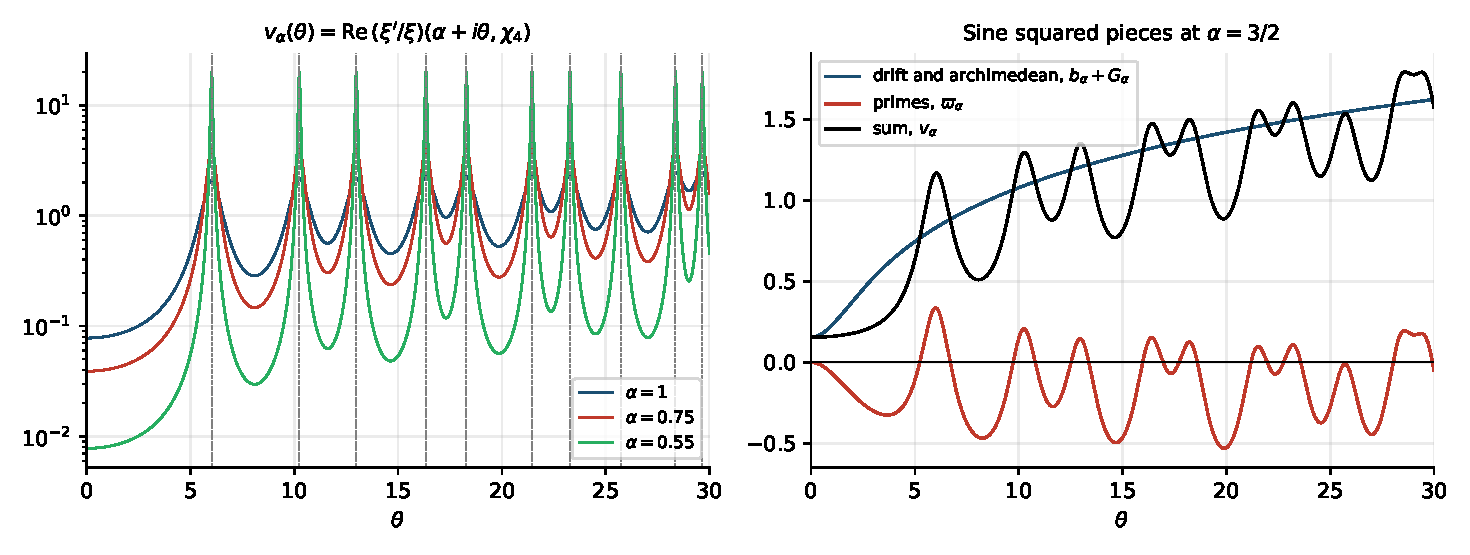
\includegraphics[width=\textwidth]{fig/dbeta_thorin.pdf}
\caption{Left: $v_\alpha(\theta)=\re(\xi'/\xi)(\alpha+i\theta,\chi_4)=\pi\rho_{\alpha-1/2}(\theta)$ for $\alpha=1$, $0.75$, $0.55$ on a logarithmic scale, with the ordinates of the zeros of $L(s,\chi_4)$ (dashed). As $\alpha\downarrow\frac12$ the density concentrates on the ordinates, while its minimum $b_\alpha$, at the origin, tends to zero. Right: at $\alpha=\frac32$, the drift and gamma piece $b_\alpha+G_\alpha$, the prime piece $\varpi_\alpha$, of both signs, and their sum $v_\alpha$. Drawn by \texttt{dbeta\_figs.py}.}
\label{fig:dbeta:thorin}
\end{figure}

\begin{proposition}\label{prop:dbeta:thorin}
For every $\alpha\ge1$, $u\mapsto\xi(\alpha,\chi_4)/\xi(\alpha+\sqrt u,\chi_4)$ is the Laplace transform of a GGC with Thorin density $v_\alpha(\theta)/\pi>0$ in the chart $\theta=\sqrt z$, and \eqref{eq:dbeta:thorinrep} holds. For $\alpha>\frac12$ it is the Laplace transform of a GGC if and only if no zero of $L(s,\chi_4)$ has real part greater than $\alpha$. GRH for $\chi_4$ holds if and only if $v_\alpha\ge0$ for every $\alpha>\frac12$, and the Thorin measures at resolution $\varepsilon=\alpha-\frac12$ converge vaguely, as $\varepsilon\downarrow0$, to the sum of the point masses $\delta_{\gamma^2}$ over the zeros on the critical line, which is the Thorin measure of $\xi(\frac12,\chi_4)/\xi(\frac12+\sqrt u,\chi_4)$ under GRH.
\end{proposition}

\begin{proof}
The proofs of Theorem~\ref{thm:poisson}, of Lagarias's criterion \cite{Lagarias} and of the vague limit stated after Remark~\ref{rem:ch2:oneline} use only the Hadamard product of an entire function of order one whose zeros are symmetric under $\rho\mapsto\bar\rho$ and $\rho\mapsto1-\rho$, with $\sum_\rho|\rho|^{-2}<\infty$; they apply to $\xi(s,\chi_4)$ \cite[Chapter 12]{Davenport}, as Section~\ref{sec:ch16:sin2} and Proposition~\ref{bp:eta:prop:thorin} apply them to $\xi(s,\chi_{12})$. Positivity at $\alpha\ge1$ needs every zero to have real part less than one, which is the absence of zeros of $L(s,\chi_4)$ on $\re s=1$ \cite[Chapter 14]{Davenport} with the Euler product and the functional equation.
\end{proof}

At the basepoint one the clock $T^{(4)}_1$, with Laplace transform $1/\xi(1+\sqrt u,\chi_4)$, therefore has the expansion $1-b_1\sqrt u+O(u)$ at the origin, and as for $\xi$ in \eqref{bp:eq:tail} the Tauberian theorem \cite[XIII.5]{Feller71} gives the tail $P(T^{(4)}_1>x)\sim(b_1/\sqrt\pi)\,x^{-1/2}=0.0438849\,x^{-1/2}$, with $b_1$ from \eqref{eq:dbeta:b1}.

Positivity at $\alpha\ge1$ uses the zeros, not the L\'evy measure. Bounding the prime weights by their absolute values gives positivity only far to the right, and no such bound does better.

\begin{proposition}\label{prop:dbeta:termwise}
For $\alpha>1$ and real $\theta$,
\begin{gather*}
v_\alpha(\theta)\ge A^\infty_4(\alpha,\theta)-S_4(\alpha),\\
A^\infty_4(\alpha,\theta)=\frac12\log\frac4\pi+\frac12\re\psi\Big(\frac{\alpha+1+i\theta}2\Big),\\
S_4(\alpha)=\sum_{n\ \mathrm{odd}}\frac{\Lambda(n)}{n^\alpha}=-\frac{\zeta'}\zeta(\alpha)-\frac{\log2}{2^\alpha-1},
\end{gather*}
and $A^\infty_4(\alpha,\theta)$ increases in $|\theta|$. The bound is positive at every $\theta$ exactly when $\alpha>\alpha_c(\chi_4)=2.2823106368$, the root of $A^\infty_4(\alpha,0)=S_4(\alpha)$. For $\chi_{12}$ the same bound, with $A^\infty_{12}(\alpha,\theta)=\frac12\log\frac{12}\pi+\frac12\re\psi(\frac{\alpha+i\theta}2)$ and $S_{12}(\alpha)=S_4(\alpha)-\log3/(3^\alpha-1)$, is positive at every $\theta$ exactly when $\alpha>\alpha_c(\chi_{12})=1.8348743295$.
\end{proposition}

\begin{proof}
For $\re s>1$,
\[
\frac{\xi'}\xi(s,\chi_4)=\frac12\log\frac4\pi+\frac12\psi\Big(\frac{s+1}2\Big)+\frac{L'}L(s,\chi_4),
\]
and $|\re\frac{L'}L(\alpha+i\theta,\chi_4)|\le\sum_n|\chi_4(n)|\Lambda(n)n^{-\alpha}=S_4(\alpha)$. The series $\re\psi(x+iy)-\psi(x)=\sum_{k\ge0}y^2/\big((x+k)((x+k)^2+y^2)\big)$ shows that $A^\infty_4$ increases in $|\theta|$. Since $A^\infty_4(\alpha,0)$ increases in $\alpha$ and $S_4(\alpha)$ decreases, the root is unique, and \texttt{dbeta\_thorin.py} locates it by bisection with certified signs. For $\chi_{12}$ the primes $2$ and $3$ drop out of the sum.
\end{proof}

In the sine squared form \eqref{eq:dbeta:sin2} the same bound reads $b_\alpha+G_\alpha(\theta)-2\sum_{\chi_4(n)=-1}\Lambda(n)n^{-\alpha}$: the positive atoms are dropped and each negative atom is given its largest value $2$ of $1-\cos$. The smaller value of $\alpha_c$ for $\chi_{12}$ reflects its larger conductor constant $\frac12\log\frac{12}\pi$ and the absence of the primes $2$ and $3$.

\begin{proposition}\label{prop:dbeta:kron}
For $\alpha>1$ and every $T>0$,
\[
\inf_{\theta\ge T}\Big(v_\alpha(\theta)-A^\infty_4(\alpha,\theta)\Big)=\inf_{\theta\ge T}\re\frac{L'}L(\alpha+i\theta,\chi_4)=-S_4(\alpha),
\]
so no lower bound for $\re\frac{L'}L(\alpha+i\theta,\chi_4)$ better than $-S_4(\alpha)$ holds at all large heights. The bound of Proposition~\ref{prop:dbeta:termwise} certifies $v_\alpha(\theta)>0$ exactly for $|\theta|>t_0(\alpha)$, where $A^\infty_4(\alpha,t_0)=S_4(\alpha)$, for $1<\alpha\le\alpha_c$ (so that $t_0(\alpha_c)=0$), and at every real $\theta$ for $\alpha>\alpha_c$, and
\[
\log t_0(\alpha)=\frac2{\alpha-1}-2\gamma_E-\log\frac8\pi+O(\alpha-1),\qquad\alpha\downarrow1,
\]
with $-2\gamma_E-\log\frac8\pi=-2.0891$.
\end{proposition}

\begin{proof}
From the Euler product, $\re\frac{L'}L(\alpha+i\theta,\chi_4)=-\sum_p\log p\,\re\frac{w_p}{1-w_p}$ with $w_p=\chi_4(p)p^{-\alpha-i\theta}$, and on the circle $|w|=r<1$ the maximum of $\re\frac w{1-w}=\re\frac1{1-w}-1$ is $\frac r{1-r}$, at $w=r$; this gives the lower bound $-S_4(\alpha)$. Since the numbers $\log p$ are linearly independent over $\mathbb Q$, Kronecker's theorem \cite[Chapter 23]{boHardyWright} gives, for every $P$ and $\eta>0$, a height $\theta\ge T$ at which $|\chi_4(p)p^{-i\theta}-1|<\eta$ for all odd $p\le P$, and the primes beyond $P$ contribute at most $\sum_{p>P}\log p\,p^{-\alpha}/(1-p^{-\alpha})$, which is small for $P$ large. For the asymptotic, $S_4(\alpha)=\frac1{\alpha-1}-\gamma_E-\log2+O(\alpha-1)$ and $A^\infty_4(\alpha,t)=\frac12\log\frac{2t}\pi+O(t^{-2})$ as $t\to\infty$, uniformly for $1\le\alpha\le2$, from $\psi(z)=\log z-\frac1{2z}+O(|z|^{-2})$; solving $A^\infty_4(\alpha,t_0)=S_4(\alpha)$ gives the formula, since $t_0(\alpha)\to\infty$.
\end{proof}

\begin{table}[htbp]
\centering\small
\begin{tabular}{cccc}
\toprule
$\alpha$ & $S_4(\alpha)$ & $t_0(\alpha)$ & $\log t_0(\alpha)-\frac2{\alpha-1}$\\
\midrule
$2$ & $0.33891193$ & $2.36723$ & $-1.1383$\\
$1.75$ & $0.57950941$ & $4.71677$ & $-1.1155$\\
$1.5$ & $1.1261406$ & $14.8728$ & $-1.3005$\\
$1.25$ & $2.9637961$ & $589.44$ & $-1.6208$\\
$1.1$ & $8.8348984$ & $7.41336\times10^7$ & $-1.8786$\\
$1.05$ & $18.784554$ & $3.25219\times10^{16}$ & $-1.9793$\\
\bottomrule
\end{tabular}
\caption{The height $t_0(\alpha)$ above which the bound of Proposition~\ref{prop:dbeta:termwise} certifies $v_\alpha>0$, for basepoints below $\alpha_c(\chi_4)=2.2823$; the last column tends to $-2\gamma_E-\log\frac8\pi=-2.0891$ (Proposition~\ref{prop:dbeta:kron}). Computed by \texttt{dbeta\_thorin.py}.}
\label{tab:dbeta:kron}
\end{table}

So for $1<\alpha<\alpha_c$ the absolute values of the weights reduce the positivity of $v_\alpha$ to a computation on $[0,t_0(\alpha)]$, but $t_0$ grows like $e^{2/(\alpha-1)}$ (Table~\ref{tab:dbeta:kron}). At $\alpha=1$ the prime piece converges only conditionally, by the prime number theorem for progressions, whose analytic input is the absence of zeros of $L(s,\chi_4)$ on $\re s=1$; the positivity of $v_1$, which Proposition~\ref{prop:dbeta:thorin} draws from that input, cannot come from the sizes of the weights. (Dirichlet's theorem for the modulus $4$ itself needs only $L(1,\chi_4)=\frac\pi4\ne0$.)

\subsubsection{The Gaussian field}\label{sec:dbeta:qi}

The pairing of the primes $p\equiv1$ and $p\equiv3\pmod4$ is their splitting in $K=\mathbb Q(i)$: a prime $p\equiv1\pmod4$ splits into two Gaussian primes of norm $p$, and a prime $p\equiv3\pmod4$ stays prime, with norm $p^2$. Accordingly $\zeta_K(s)=\zeta(s)L(s,\chi_4)$, and in the normalisation of Section~\ref{sec:sqfree:nf},
\[
\xi_K(s)=2s(s-1)\pi^{-s}\Gamma(s)\zeta_K(s)=\xi(s)\,\xi(s,\chi_4),
\]
by the duplication formula $\Gamma(s)=2^{s-1}\pi^{-1/2}\Gamma(\frac s2)\Gamma(\frac{s+1}2)$. Write $v^K_\alpha$ and $v^\xi_\alpha$ for the brackets $\re(\xi_K'/\xi_K)(\alpha+i\theta)$ and $\re(\xi'/\xi)(\alpha+i\theta)$, and $v_\alpha$ as before for $\chi_4$.

\begin{proposition}\label{prop:dbeta:factor}
On every vertical line, $v_\alpha=v^K_\alpha-v^\xi_\alpha$. For $\alpha>1$ the canonical measure of $\xi_K$ at the basepoint $\alpha$ is
\[
x\Pi^K_\alpha(dx)=\Big(\frac{e^{-(\alpha+1)x}}{1-e^{-x}}-e^{-(\alpha-1)x}\Big)dx+\sum_{n\ge2}\frac{(1+\chi_4(n))\Lambda(n)}{n^\alpha}\,\delta_{\log n}(dx),
\]
and the canonical measure of Proposition~\ref{prop:dbeta:levy} is $x\Pi_\alpha=x\Pi^K_\alpha-x\Pi^\xi_\alpha$, with $x\Pi^\xi_\alpha$ that of Section~\ref{bp:sec:levy}: the pole densities $-e^{-(\alpha-1)x}$ cancel, the gamma densities differ by $e^{-\alpha x}/(2\sinh x)$, and the atoms by $\chi_4(n)\Lambda(n)n^{-\alpha}$.
\end{proposition}

\begin{proof}
Take logarithmic derivatives in $\xi_K=\xi\cdot\xi(\cdot,\chi_4)$. For the measures write $\xi_K(s)=(s-1)\cdot2\pi^{-s}\Gamma(s+1)\zeta_K(s)$: Binet's formula for $\Gamma(s+1)$ at $\alpha$ gives the density $e^{-(\alpha+1)x}/(x(1-e^{-x}))$, the factor $s-1$ gives $-e^{-(\alpha-1)x}/x$ as for $\xi$, and $-\frac{\zeta_K'}{\zeta_K}=-\frac{\zeta'}\zeta-\frac{L'}L$ has the coefficients $(1+\chi_4(n))\Lambda(n)\ge0$. Finally $\frac{e^{-(\alpha+1)x}}{1-e^{-x}}-\frac{e^{-(\alpha+2)x}}{1-e^{-2x}}=e^{-\alpha x}\Big(\frac1{e^x-1}-\frac1{e^{2x}-1}\Big)=\frac{e^{-\alpha x}e^x}{e^{2x}-1}=\frac{e^{-\alpha x}}{2\sinh x}$.
\end{proof}

\begin{corollary}\label{cor:dbeta:dom}
\textup{(i)} For every $\alpha\ge1$ there are independent GGC variables $H^\xi_\alpha$ and $H^{(4)}_\alpha$, with Laplace transforms $\xi(\alpha)/\xi(\alpha+\sqrt u)$ and $\xi(\alpha,\chi_4)/\xi(\alpha+\sqrt u,\chi_4)$, whose sum $H^K_\alpha=H^\xi_\alpha+H^{(4)}_\alpha$ is the GGC with Laplace transform $\xi_K(\alpha)/\xi_K(\alpha+\sqrt u)$ and Thorin density $v^K_\alpha/\pi$.

\textup{(ii)} GRH for $\chi_4$ holds if and only if $v^K_\alpha\ge v^\xi_\alpha$ on every line $\re s=\alpha>\frac12$: the Thorin density of $\xi_K$ dominates that of $\xi$ at every basepoint.

\textup{(iii)} Under RH, GRH for $\chi_4$ holds if and only if, for every $\alpha>\frac12$, $\xi_K(\alpha)/\xi_K(\alpha+\sqrt u)$ is the Laplace transform of $H^\xi_\alpha+H$ for some GGC $H$ independent of $H^\xi_\alpha$.
\end{corollary}

\begin{proof}
(i) By Theorem~\ref{thm:poisson} and Proposition~\ref{prop:dbeta:thorin} both factors are GGC transforms for $\alpha\ge1$, and transforms of independent sums multiply. (ii) By Proposition~\ref{prop:dbeta:factor}, $v^K_\alpha\ge v^\xi_\alpha$ is $v_\alpha\ge0$, and Proposition~\ref{prop:dbeta:thorin} applies. (iii) Under RH, $H^\xi_\alpha$ is a GGC for every $\alpha>\frac12$ (Theorem~\ref{thm:poisson}). If GRH holds for $\chi_4$, take $H=H^{(4)}_\alpha$. Conversely, the transform of $H$ is then $\xi(\alpha,\chi_4)/\xi(\alpha+\sqrt u,\chi_4)$, and if it is a GGC transform for every $\alpha>\frac12$, Proposition~\ref{prop:dbeta:thorin} gives GRH.
\end{proof}

Neither $v^K_\alpha$ nor $v^\xi_\alpha$ is positive term by term: each has the pole piece $-\theta^2/\big((\alpha-1)((\alpha-1)^2+\theta^2)\big)$ of \eqref{eq:split}, and the two cancel in the difference, which is why $\xi(s,\chi_4)$ has none. The factorisation is the right language for the pairing of the primes, but it does not by itself lower $\alpha_c$: by Proposition~\ref{prop:dbeta:kron} any argument that uses only the sizes of the weights reaches no further. Table~\ref{tab:dbeta:qi} shows the three brackets at $\alpha=\frac32$; \texttt{dbeta\_thorin.py} checks $v^K_\alpha-v^\xi_\alpha-v_\alpha=0$ there to $10^{-36}$, and the identity $\xi_K=\xi\cdot\xi(\cdot,\chi_4)$ at $s=0.3+4.1i$, where both sides are $0.21807580405390-0.037869233276222i$ after division by $\xi(s)$, and at $s=2.5$.

\begin{table}[htbp]
\centering\small
\begin{tabular}{cccccc}
\toprule
$\theta$ & $0$ & $2$ & $5$ & $10$ & $20$\\
\midrule
$v^K_{3/2}(\theta)$ & $0.200351$ & $0.225243$ & $0.685189$ & $1.32766$ & $1.49863$\\
$v^\xi_{3/2}(\theta)$ & $0.0461359$ & $0.0470396$ & $0.0526739$ & $0.102889$ & $0.606114$\\
$v_{3/2}(\theta)$ & $0.154215$ & $0.178204$ & $0.632515$ & $1.22477$ & $0.892517$\\
\bottomrule
\end{tabular}
\caption{The brackets of $\xi_{\mathbb Q(i)}$, $\xi$ and $\xi(\cdot,\chi_4)$ at the basepoint $\frac32$; the last row is the difference of the first two (Proposition~\ref{prop:dbeta:factor}). Computed by \texttt{dbeta\_thorin.py}.}
\label{tab:dbeta:qi}
\end{table}

The same holds for every real primitive character $\chi_D$, with $D$ a fundamental discriminant and $K=\mathbb Q(\sqrt D)$: $\xi_K$ is a constant multiple of $\xi\cdot\xi(\cdot,\chi_D)$, the constant being $2/\sqrt{|D|}$ for $D<0$ (Section~\ref{sec:sqfree:quad}) and $2$ for $D>0$, since then $\xi_K(s)=s(s-1)D^{s/2}\Gamma_{\mathbb R}(s)^2\zeta_K(s)$ and $\xi(s,\chi_D)=D^{s/2}\Gamma_{\mathbb R}(s)L(s,\chi_D)$. So $v^{(\chi_D)}_\alpha=v^K_\alpha-v^\xi_\alpha$; the GGC property at every $\alpha\ge1$, the equivalence of GRH for $\chi_D$ with the domination of the Thorin density of $\xi$ by that of $\xi_K$, and the localisation of Corollary~\ref{cor:dbeta:argmono} hold for $\xi(s,\chi_D)$ with the same proofs. For $\chi_{12}$, $K=\mathbb Q(\sqrt3)$, and the numbers are: $\alpha_c(\chi_{12})=1.8348743295$ (Proposition~\ref{prop:dbeta:termwise}); $V_{12}=(\log\xi)''(\frac12,\chi_{12})=0.332923608212$; and at $\alpha=1$, $0.75$ and $0.6$ the drift $b_\alpha$ is $0.1650833$, $0.0830566$ and $0.0332812$, the minimum of $v_\alpha$ on a grid of step $0.01$ on $[0,60]$, attained at the origin (\texttt{dbeta\_minimum.py}), as Theorem~\ref{thm:dbeta:minall} proves at every height for $\alpha\ge1$ and on the verified range for $\frac12<\alpha<1$. The script \texttt{dbeta\_zeros.py} certifies the first five ordinates of $L(s,\chi_{12})$, $3.8046276331$, $6.6922233205$, $8.8905929587$, $11.1883927451$ and $12.9661788080$, all simple and on the critical line, in agreement with Section~\ref{sec:ch16:eta}; their largest gap, the first, $2.8876$, lies below $2/\sqrt{V_{12}}=3.4662$, and below the value $3.3189$ at $a=\frac12$ of the threshold of Remark~\ref{rem:dbeta:nearest} for $\chi_{12}$. On the real axis the same script gives $L(\sigma,\chi_{12})=0.1246437042$, $0.3344871142$, $0.4985570025$, $0.6250274399$ and $0.7213905658$ at $\sigma=0.1$, $0.3$, $0.5$, $0.7$ and $0.9$, positive, as the positivity of the kernel requires.

\begin{question}\label{q:dbeta:coupling}
Is there a construction of $H^K_\alpha=H^\xi_\alpha+H^{(4)}_\alpha$ from the Gaussian primes themselves, two of norm $p$ for each $p\equiv1$ and one of norm $p^2$ for each $p\equiv3\pmod4$, that persists below the basepoint one? By Proposition~\ref{prop:dbeta:kron} such a construction must see the phases $p^{-i\theta}$, not only the sizes of the weights; below $\alpha=1$ its existence is equivalent to GRH for $\chi_4$ under RH, by Corollary~\ref{cor:dbeta:dom}(iii). In the language of Section~\ref{sec:dbeta:arg}, the decomposition is the additivity $\arg\xi_K=\arg\xi+\arg\xi(\cdot,\chi_4)$ on vertical lines, and the domination of Corollary~\ref{cor:dbeta:dom}(ii) says that $\arg\xi_K-\arg\xi$ is nondecreasing on every line $\re s=\alpha>\frac12$.
\end{question}

\subsubsection{The Thorin measure as an argument}\label{sec:dbeta:arg}

The density $v_\alpha(\theta)$ is the derivative in $\theta$ of the argument of $\xi(\alpha+i\theta,\chi_4)$, so the Thorin measure on a vertical line is an argument, and at the centre a zero count.

\begin{proposition}\label{prop:dbeta:arg}
Let $\alpha>\frac12$ be such that no zero of $\xi(s,\chi_4)$ lies on the line $\re s=\alpha$; this holds for every $\alpha\ge1$. Then for $\theta>0$
\[
\frac1\pi\int_0^\theta v_\alpha(t)\,dt=\frac1\pi\arg\xi(\alpha+i\theta,\chi_4),
\]
with the argument continuous along the segment from $\alpha$ to $\alpha+i\theta$ and zero at $\alpha$; for $\alpha\ge1$ the left side is the mass of $(0,\theta^2]$ under the Thorin measure of Proposition~\ref{prop:dbeta:thorin}. As $\theta\to\infty$, with $a=\frac{\alpha+1}2$,
\[
\frac1\pi\arg\xi(\alpha+i\theta,\chi_4)=\frac\theta{2\pi}\log\frac{2\theta}{\pi e}+\frac\alpha4+\frac1\pi\arg L(\alpha+i\theta,\chi_4)-\frac{a(a-1)+\frac16}{\pi\theta}+O(\theta^{-3}),
\]
with $\arg L$ continuous along the same segment. As $\alpha\downarrow\frac12$, for $\theta$ not an ordinate, the left side tends to the number of zeros on the critical line with $0<\gamma<\theta$, which is $N(\theta)$ under GRH; at $\alpha=\frac12$ the expansion is the counting formula \eqref{eq:dbeta:count}.
\end{proposition}

\begin{proof}
Since $\frac{d}{dt}\log\xi(\alpha+it,\chi_4)=i\frac{\xi'}\xi(\alpha+it,\chi_4)$, the derivative of $\arg\xi(\alpha+it,\chi_4)=\im\log\xi(\alpha+it,\chi_4)$ is $v_\alpha(t)$, and $\xi(\alpha,\chi_4)>0$. The expansion is $\frac\theta2\log\frac4\pi$ plus Stirling's series $\log\Gamma(z)=(z-\frac12)\log z-z+\frac12\log2\pi+\frac1{12z}+O(|z|^{-3})$ \cite[\S5.11]{DLMF} at $z=a+\frac{i\theta}2$: with $y=\frac\theta2$,
\[
\im\log\Gamma(a+iy)=y\log y-y+\frac\pi2\Big(a-\frac12\Big)-\Big(\frac{a(a-1)}2+\frac1{12}\Big)\frac1y+O(y^{-3}),
\]
from $\arg z=\frac\pi2-\frac ay+O(y^{-3})$ and $\log|z|=\log y+\frac{a^2}{2y^2}+O(y^{-4})$; and $\frac\theta2\log\frac4\pi+\frac\theta2\log\frac\theta2-\frac\theta2=\frac\theta2\log\frac{2\theta}{\pi e}$, $\frac12(a-\frac12)=\frac\alpha4$. For the limit, write $v_\alpha$ by the Hadamard product, as in Proposition~\ref{prop:struct}, as the absolutely convergent sum over the zeros $\rho=\beta+i\gamma$ of $(\alpha-\beta)/((\alpha-\beta)^2+(t-\gamma)^2)$; each term integrates over $[0,\theta]$ to $\arctan\frac{\theta-\gamma}{\alpha-\beta}+\arctan\frac\gamma{\alpha-\beta}$, which for a zero on the line tends to $\pi$ if $0<\gamma<\theta$ and to $0$ if $\gamma>\theta$ or $\gamma<0$, while the two terms of an off line pair $\frac12\pm\delta+i\gamma$ have the limits $\mp\big(\arctan\frac{\theta-\gamma}\delta+\arctan\frac\gamma\delta\big)$, which cancel. The terms are dominated by $\pi$ and by $C\theta/\gamma^2$ for $|\gamma|>2\theta+1$, uniformly for $\frac12<\alpha\le1$, so dominated convergence applies. At $\alpha=\frac12$, $a=\frac34$ and $a(a-1)+\frac16=-\frac1{48}$.
\end{proof}

The Thorin measure at resolution $\varepsilon=\alpha-\frac12$ is therefore the zero counting function smoothed by the Cauchy kernel of width $\varepsilon$; this is the analogue for $\chi_4$ of the cumulative Thorin mass of $\xi$ as a smoothed counting function (Section~\ref{sec:ch9:mass}). The script \texttt{dbeta\_thorin.py} continues $\arg\xi(\alpha+i\theta,\chi_4)$ in ball arithmetic, as \texttt{dbeta\_zeros.py} does, and integrates $v_\alpha$ by quadrature: at $(\alpha,\theta)=(1.5,10)$, $(1.5,25)$ and $(2,30)$ both sides are $1.65731473994$, $7.40149777268$ and $9.85153586211$. At $\alpha=0.75$ the difference between the left side and the first three terms of the expansion is $-3.65\times10^{-4}$, $-1.82\times10^{-4}$ and $-9.12\times10^{-5}$ at $\theta=50$, $100$ and $200$, that is $-0.0182/\theta$, against $-(a(a-1)+\frac16)/\pi=-11/(192\pi)=-0.018237$ at $a=\frac78$.

\begin{corollary}\label{cor:dbeta:argmono}
GRH for $\chi_4$ holds if and only if, for every $\alpha>\frac12$, $\theta\mapsto\arg\xi(\alpha+i\theta,\chi_4)$ is nondecreasing. With no hypothesis, the heights $\theta>0$ at which it decreases lie in the union of the windows $|\theta-\gamma|<\sqrt{\delta^2-(\alpha-\frac12)^2}$, each of length less than $1$, over the zeros $\frac12+\delta+i\gamma$ with $\delta>\alpha-\frac12$, and there are none at heights below $2.5\times10^7-\frac12$.
\end{corollary}

\begin{proof}
The derivative is $v_\alpha(\theta)$, and Proposition~\ref{prop:dbeta:thorin} gives the equivalence. By the Hadamard product, $v_\alpha$ is a sum of positive Cauchy kernels, one for each zero on the line and two for each off line pair $\frac12\pm\delta+i\gamma$ with $\delta\le\alpha-\frac12$, plus, for each pair with $\delta>\alpha-\frac12$, the difference $\pi\big(P_{\varepsilon+\delta}-P_{\delta-\varepsilon}\big)(\theta\mp\gamma)$ with $\varepsilon=\alpha-\frac12$, which is negative exactly where $|\theta\mp\gamma|<\sqrt{\delta^2-\varepsilon^2}$ (proof of Proposition~\ref{prop:signature}(ii)); for $\theta>0$ and $\gamma>0$ the reflected term at $\theta+\gamma$ is positive, since $\theta+\gamma>\gamma>\delta$. A window has length $2\sqrt{\delta^2-\varepsilon^2}<2\delta<1$. Platt's verification of GRH for the modulus $4$ to height $10^8/4$ \cite{Platt16} puts every zero off the line above $2.5\times10^7$, and so every window above $2.5\times10^7-\frac12$.
\end{proof}

A window holds a decrease only if the negative term of its pair outweighs all the positive terms there, and the decrease is bounded: the negative part of the term $\pi(P_{\varepsilon+\delta}-P_{\delta-\varepsilon})(\theta-\gamma)$ of a pair has integral $4\arctan\sqrt{(\delta+\varepsilon)/(\delta-\varepsilon)}-\pi<\pi$, by Proposition~\ref{prop:signature}(iii), so over any interval the argument falls by less than $\pi$ times the number of pairs whose windows meet it, whatever the other zeros, and the fall caused by a pair tends to zero as $(\alpha-\frac12)/\delta\to0$. This answers the quantitative half of a question of the first author's note. No lower bound for the positive terms over a window, such as a mean value estimate for the contribution of the zeros on the line, can exclude this for every pair: at the centre $\theta=\gamma$ of its window the pair contributes $\frac1{\varepsilon+\delta}-\frac1{\delta-\varepsilon}=-\frac{2\varepsilon}{\delta^2-\varepsilon^2}$, which is unbounded below as $\delta\downarrow\varepsilon$, that is as the zero approaches the line $\re s=\alpha$ from the right, while by Lemma~\ref{ag:lem:cancel} a zero far enough to the right of the line cannot produce a decrease against a given positive floor. Outside the strips $|\theta-\gamma|<(1+\sqrt2)\delta$ around the ordinates of the zeros off the line, Theorem~\ref{thm:dbeta:comp} gives the argument a rate of increase that grows like $\log\theta$ (Corollary~\ref{cor:dbeta:lower}). Figure~\ref{fig:dbeta:arg} shows the smoothing, and the minimum at the origin that Section~\ref{sec:dbeta:comp} proves.

\begin{figure}[htbp]
\centering
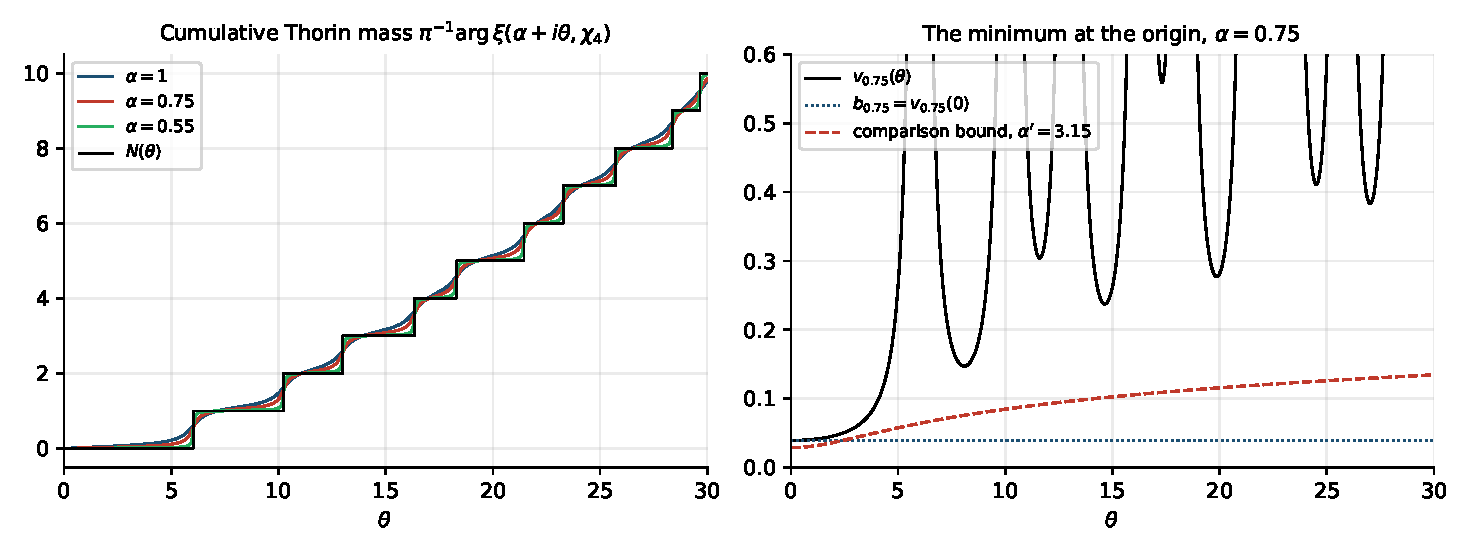
\includegraphics[width=\textwidth]{fig/dbeta_argument.pdf}
\caption{Left: the cumulative Thorin mass $\frac1\pi\arg\xi(\alpha+i\theta,\chi_4)=\frac1\pi\int_0^\theta v_\alpha$ for $\alpha=1$, $0.75$ and $0.55$, against the zero count $N(\theta)$ of $L(s,\chi_4)$; at $\theta=30$ the masses are $9.7747$, $9.8405$ and $9.9621$, and $N(30)=10$. The argument is continued through the quotients of values at steps of $0.005$, each of argument below $0.11$ in modulus. Right: $v_{0.75}(\theta)$, its minimum $b_{0.75}=0.0389784$ at the origin, and the lower bound of Corollary~\ref{cor:dbeta:lower} with $\alpha'=3.15$, which exceeds $b_{0.75}$ for $\theta>2.434$ (\texttt{dbeta\_minimum.py}). Drawn by \texttt{dbeta\_figs.py}.}
\label{fig:dbeta:arg}
\end{figure}

\subsubsection{The centre}\label{sec:dbeta:centre}

For $\zeta$ the positive structure at the centre is the Thorin measure of the clock, not a structure of the P\'olya variable itself (Proposition~\ref{sb:prop:qid}(1)). The same holds for $\chi_4$. The characteristic function $\xi(\frac12+i\theta,\chi_4)/\xi(\frac12,\chi_4)$ of $Y_4$ is real and changes sign at $\gamma_1=6.0209489$, where it passes from $0.00607732$ at $\theta=5.9$ to $-0.00350813$ at $\theta=6.1$, and at each of the other ordinates below height $100$; Hardy's argument for $\zeta$ \cite[Chapter 10]{Titchmarsh}, applied to the theta series $\eta(ix)^3$ of $\chi_4$, gives infinitely many such sign changes. So $Y_4$ is not quasi infinitely divisible, and in particular not infinitely divisible: a quasi infinitely divisible characteristic function never vanishes. Nor is $\xi(\frac12+w,\chi_4)/\xi(\frac12,\chi_4)$ a positive mixture $\int M(d\lambda)/(w+\lambda)^2$ of Gamma(2) transforms, for a more elementary reason: such a mixture decreases on $w>0$, while $\xi(\frac12+w,\chi_4)=\int_{\R}K_4(u)\cosh(wu)\,du$ increases there. A one sided object remains, the half kernel $K_4(u)\mathbf 1\{u>0\}$, and it is not a positive gamma mixture either.

\begin{proposition}\label{prop:dbeta:nocm}
For no $a>0$ is $u^{1-a}K_4(u)$ completely monotone on $u>0$; in particular the half kernel is not a positive mixture of Gamma($a$) densities $u^{a-1}e^{-\lambda u}$, for any shape $a$. The theta function $\eta(ix)^3$ is not completely monotone on $x>0$.
\end{proposition}

\begin{proof}
If $g(u)=\int_{[0,\infty)}e^{-\lambda u}M(d\lambda)$ with $M\ge0$ and $M\ne0$, choose $L$ with $M([0,L])>0$; then $g(u)\ge M([0,L])e^{-Lu}$, so $g$ decays at most exponentially, while $u^{1-a}K_4(u)$ decays like $\exp(-\frac\pi4e^{2u})$ (Proposition~\ref{prop:dbeta:kernel}). The Jacobi series $\eta(ix)^3=\sum_{n\ge0}(-1)^n(2n+1)e^{-\pi(2n+1)^2x/4}$ is the Laplace transform of the signed measure with the weights $(-1)^n(2n+1)$ at the points $\pi(2n+1)^2/4$, which by the uniqueness of the Laplace transform is its only representing measure, and it is not positive, so Bernstein's theorem excludes complete monotonicity.
\end{proof}

The decay argument applies to the kernel of every completed $L$ function of degree one, all of which decay like $\exp(-ce^{2|u|})$; for $\xi$ it shows that no positive mixture of Gamma($a$) densities represents the P\'olya kernel on the half line, for any shape $a$, as \cite[Section 13.6]{P17} observes (see also \cite[Section 12.6]{P26}).

The positive structure is in the reciprocal of the product. With $q=e^{-2\pi x}$,
\begin{equation}\label{eq:dbeta:recip}
\frac{e^{-\pi x/4}}{\eta(ix)^3}=\prod_{m\ge1}\big(1-q^m\big)^{-3}=\exp\Big(3\sum_{N\ge1}\sigma_{-1}(N)\,e^{-2\pi Nx}\Big),\qquad\sigma_{-1}(N)=\sum_{d\mid N}\frac1d,
\end{equation}
from $-\log(1-q^m)=\sum_kq^{mk}/k$; so the logarithm of the left side is completely monotone, and hence so is the left side, the exponential of a completely monotone function being completely monotone. At $x=0.3$ the three forms agree to fifteen digits, $1.77964734678018$ (\texttt{dbeta\_thorin.py}). In the language of Section~\ref{sec:ch16:max}, $\prod_m(1-e^{-2\pi mx})^3$ is the distribution function of the maximum $M_3$ of independent exponential variables, three of each rate $2\pi m$, and \eqref{eq:dbeta:recip} is the complete monotonicity of minus the logarithm of such a distribution function noted in Section~\ref{sec:ch16:dbn}, with the masses $3\sigma(N)/N$. The representation of Section~\ref{sec:ch16:max} also carries over: since $\eta(ix)^3=e^{-\pi x/4}\Pr(M_3\le x)$ and $x^{c-1}e^{-\pi x/4}(\pi/4)^c/\Gamma(c)$ is the density of $\frac4\pi G_c$, with $G_c$ a gamma variable of shape $c$ independent of $M_3$, the Mellin form gives $\xi(s,\chi_4)=(\frac4\pi)^c\Gamma(c)\Pr(\frac4\pi G_c\ge M_3)$ with $c=\frac{s+1}2$, that is
\[
L(s,\chi_4)=\Pr\big(4G_{(s+1)/2}\ge\pi M_3\big),\qquad s>-1,
\]
which at $s=1$ is $\E e^{-\pi M_3/4}=\frac\pi4\int_0^\infty\eta(ix)^3dx=\frac\pi4$.

The half kernel has the Laplace transform
\begin{equation}\label{eq:dbeta:incomplete}
\int_0^\infty e^{-wu}K_4(u)\,du=A_4\big(\tfrac12-w\big),
\end{equation}
where
\[
A_4(s)=\int_1^\infty\eta(ix)^3x^{(s+1)/2}\frac{dx}x=\sum_{n\ge1}\chi_4(n)\,n\,\frac{\Gamma(\frac{s+1}2,\frac{\pi n^2}4)}{(\pi n^2/4)^{(s+1)/2}}
\]
is an incomplete Mellin transform of $\eta^3$, and the transformation $\eta(i/x)^3=x^{3/2}\eta(ix)^3$, applied to the integral over $(0,1)$, gives $\xi(s,\chi_4)=A_4(s)+A_4(1-s)$ for every $s$. This is the analogue of Riemann's formula (Proposition~\ref{prop:maxexp:riemann}) and of the symmetric form \eqref{eq:maxexp:sym} for $\Delta$, with no pole terms, since $\eta(ix)^3$ has no constant term. At $w=0.3$ both sides of \eqref{eq:dbeta:incomplete} are $0.44608019686738$, and $A_4(0.2)+A_4(0.8)=\xi(0.2,\chi_4)=0.98762005303445$ (\texttt{dbeta\_thorin.py}).

\begin{question}\label{q:dbeta:recip}
Can the complete monotonicity of \eqref{eq:dbeta:recip}, and of its analogue $\prod_m(1-q^m)^{-1}$ for the kernel of $\chi_{12}$, be turned into a positive representation on the reciprocal side, in the spirit of Thorin's construction for the reciprocal of a GGC transform?
\end{question}
